% This template was originally by R. Jacob Vogelstein
% Updated on March 1, 2010 by Noah J. Cowan

% Brian began working on thesis on February 2, 2017

\documentclass[12pt,oneside,final]{thesis}

%\usepackage[superscript]{cite} %bh commented out
\usepackage{amsmath,amsfonts}
\usepackage{graphicx}
\graphicspath{{./figs/}}
\usepackage{fixltx2e}
\usepackage{array}
% wrapfig is fragile: use sparingly
\usepackage{wrapfig} 
%\usepackage{times}  % Use this for ugly fonts

\usepackage{upgreek}
%\usepackage{hyperref} % bh commented out
\usepackage{setspace}

\usepackage{booktabs}
\usepackage{multirow}
\usepackage{longtable}
\usepackage[font=singlespacing, labelfont=bf]{caption}
%\usepackage{CV}

\usepackage{enumitem}
\newlist{inlinelist}{enumerate*}{1}
\setlist*[inlinelist,1]{%
  label=(\arabic*),
}

\usepackage{fancyhdr}    % Use nice looking headers along with the required footer page numbers   
%\usepackage[hypertex]{hyperref}

%Define the header/footer style
\pagestyle{fancy}
\fancyhf{}
\setlength{\headheight}{15pt}
\lhead{\leftmark}
\cfoot{\thepage}
\renewcommand{\headrulewidth}{0pt}
\fancypagestyle{plain}{% Redefine ``plain'' style for chapter boundaries
\fancyhf{} % clear all header and footer fields
\fancyfoot[C]{\thepage} % except the center
\renewcommand{\headrulewidth}{0pt}
\renewcommand{\footrulewidth}{0pt}}

%\tolerance=10000

%\makeglossary % enable the glossary


% Ernst's customary preamble definitions
\long\def\comment#1{} %%% to comment out a section of text
\usepackage{xspace}
\newcommand{\ie}[0]{{\em i.e.}\ }
\newcommand{\eg}[0]{{\em e.g.}\ }
\newcommand{\etal}[0]{{\em et al.}\xspace}
\newcommand{\etc}[0]{{\em etc.}\xspace}
\newcommand{\vs}[0]{{\em vs.}\xspace}
\newcommand{\vv}[0]{{\em vice-versa}\xspace}
\newcommand{\via}[0]{{\em via}\xspace}
\newcommand{\ibid}[0]{{\em ibid}\xspace}

% bh Useful additions to the base thesis template
\usepackage{pdfpages} % for including personal CV as pdf at end of file (replaces default CV)
\usepackage[round,authoryear]{natbib} % for author-year citations (replaces default cite)
\usepackage[titletoc,title]{appendix} % change appendix behavior
\usepackage{siunitx} % for reporting small p-values
\def\newblock{\hskip .11em plus .33em minus .07em} % needed to get bibliography working

% bh For pdf/a compatibility
\usepackage[pdfa]{hyperref}

% bh Compile chapters separately (comment out for full thesis)
\includeonly{chapter0,Intro/chapter1,Contour/chapter2,NaturalImage/chapter3,3D-Surface/chapter4,3D-Saliency/chapter5,conclusion,appendix} % missing natural grouping chapter and conclusion


\begin{document}

\title{Grouping mechanisms for object-based vision and attention}
\author{Brian H. Hu}
\degreemonth{August}
\degreeyear{2017} 
\dissertation
\doctorphilosophy
\copyrightnotice


% add your chapters, best way is to have separate TeX files for each chapter
%%% FRONTMATTER
\begin{frontmatter}

% generate title
\maketitle

\begin{abstract}
% bh taken from NRSA/thesis proposal specific aims
% Chapter 1: Introduction
% Chapter 2: Contour Integration/Border Ownership
% Chapter 3: Figure-Ground Organization in Natural Scenes
% Chapter 4: 3D Surface Representation (Basis Functions)
% Chapter 5: 3D Proto-object Based Saliency
  
The visual brain faces the difficult task of reconstructing a three-dimensional (3D) world from two-dimensional (2D) images projected onto the two retinae. In doing so, visual information is organized in terms of objects in 3D space, and this organization is the basis for visual perception. In complex visual scenes, both the foreground and the background are rich in features of different types. The brain must find a way to group together the features that belong to objects on the foreground and distinguish them from features in the background.

The goal of this thesis is to understand how the neural circuits in primate cortex accomplish this task using grouping mechanisms for object-based vision and attention. Through computational modeling, I show that grouping mechanisms are fundamental for linking early feature representations to tentative perceptual objects known as proto-objects. Previous models on the neural coding of border ownership have identified a plausible network architecture for proto-object based perceptual organization. I extend these models to explain how the same grouping model framework can be used to perform contour integration, border-ownership assignment, grouping of 3D surfaces, and computation of 3D visual saliency. My models offer several falsifiable predictions which can be tested in future experiments. My models also clarify how top-down attention interfaces with the neural circuits responsible for grouping together the features of an object. Overall, the models developed address the important question of how visual features are grouped into 2D and 3D object representations.

\vspace{1cm}

\noindent Primary Reader: Ernst Niebur\\
Secondary Reader: R{\"u}diger von der Heydt

\end{abstract}

\begin{acknowledgment}

I had the privilege of sailing with Ernst to the neuroscience retreat one year. As I was sitting on the boat, I thought about how the trip was really a metaphor for my PhD. I have had opportunities to steer the boat (sometimes in the wrong direction!) and I have gone through both good and bad weather. Through it all, I am thankful to have had Ernst as my captain.

I would like to thank my family for their continued love and support. I thank my wife, Mingming, and my daughter, Katherine, for bearing with me in these final months. I thank my parents, Benjamin and Jennifer, for the sacrifices they made for me and my siblings. I thank my brother Blair for his moral support and my sister Joy for being an inspiration to me.

I would also like to thank my thesis committee members, R{\"u}diger and Kechen, for their help and guidance during my PhD. Finally, I would like to thank my friend Matthew, for all the lunches and discussions we shared together, and my labmates Danny and Grant, who made each day in lab an interesting one.

\textbf{Soli Deo Gloria}

\vspace{-1cm} % remove extra white space to keep on one page

\end{acknowledgment}

\begin{dedication}
 
This thesis is dedicated to Joy, who first got me interested in the study of vision. Your perseverance in the face of adversity has been my inspiration.

\end{dedication}

% generate table of contents
\tableofcontents

% generate list of tables
\listoftables

% generate list of figures
\listoffigures

\end{frontmatter}

%%% Local Variables:
%%% mode: latex
%%% TeX-master: "root"
%%% End:

%\chapter{Introduction}
\label{sec:intro}
\chaptermark{Introduction}

%Introduction.

\section{Segmentation and figure-ground organization}

The task of partitioning an image into regions bounded by contours (segmentation) and the task of assigning border ownership of these contours to either the foreground or the background (figure-ground organization) are important first steps in achieving image understanding. Gestalt psychologists were the first to recognize the importance of the whole in influencing perception of the parts, and with this observation, laid out several principles for figure-ground organization~\citep{Koffka35, Wertheimer23}. For example, the rule of good continuation states that well-aligned contour elements should be grouped together. This is closely related to the concept of a ``local association field,'' where collinear contour elements excite each other and noncollinear elements inhibit each other~\citep{Ullman92, Field_etal93}. Results from neuroanatomy lend support to these ideas, as the lateral connections within V1 predominantly link similar-orientation cortical columns. However, our understanding of the neural mechanisms of these processes remains surprisingly limited.
 
The brain must keep track of which regions and contours belong to which objects. This is known as the binding problem, as it is not clear how the features of an object are bound together~\citep{Treisman96b}. One class of models relies on the fast temporal coding structures of spike trains \citep{Singer99b}, but experimental evidence is controversial~\citep{Thiele_Stoner03,Roelfsema_etal04,Dong_etal08a}. Another solution involves differential neural activity, where the neurons responding to the features of an object show increased firing compared with neurons responding to the background. This response enhancement is known as figure-ground modulation (FGM), and was first observed in primary visual cortex (V1) for texture-defined figures~\citep{Lamme95}. Similar results have been found using other tasks and techniques, including more recent voltage-sensitive dye imaging of populations of neurons during a contour grouping task~\citep{Gilad_etal13}.

However, this solution only works if there is a single object in the foreground, as multiple objects each labeled with higher neural activity could be interpreted as parts of a single object. Furthermore, each neuron's firing rate is inherently ambiguous, as higher activity could be due to labeling with FGM or because the neuron's preferred feature falls within its receptive field. As a result, the binding problem cannot be solved with models that only represent object information in terms of enhanced neural activity in early visual areas~\citep{Niebur00a}. This strongly points to neural circuits that employ populations of neurons which explicitly represent (\ie in their firing rate) the organization of the visual scene in terms of perceptual objects.

\section{The role of cortical feedback}

\comment{The resulting computational model developed by~ \citet{Stemmler_etal95b} has since been corroborated by a large number of independent studies~\citep[e.g.][]{Simonotto_etal97,Polat_etal98,Chatterjee_etal11,Xie_etal14}.}
%
Early computational models~\citep{Stemmler_etal95b} and experimental studies~\citep{Simonotto_etal97,Polat_etal98,Chatterjee_etal11,Xie_etal14} put forth the view that horizontal connections
% However, in agreement with others at the time, the underlying concept of horizontal connections in that model was that they
are essentially static, or varying over time scales given by ontogenetic development or neuronal plasticity. Such structures could thus implement overall statistics of natural scenes~\citep[like circular structures, e.g.][]{Sigman_etal01} but they could not flexibly represent the myriad of instantaneously present and constantly changing visual shapes observed during perception of dynamic scenes. This view has been considerably enlarged over the last decade or so, and what is emerging is a view in which the lateral connections are in place but can be actively and rapidly modulated by top-down connectivity from higher areas.

The degree of collinear facilitation observed in V1 is strongly context-dependent, and can change with the behavioral task~\citep{Li_etal04, Li_etal06} as well as perceptual learning~\citep{Li_etal08a, Yan_etal14}. As a result, feedback connections from higher areas may play an important role in shaping the responses of neurons in early visual areas. In fact, simultaneous neural recordings from areas V1 and V4 during two different figure-ground segregation tasks show that V4 is intimately involved in the FGM process~\citep{Poort_etal12, Chen_etal14}. In these studies, the FGM signal appears first in V4 and is then fed back to V1, with a delay representing recurrent processing. Additional studies of curve-tracing~\citep{Roelfsema_etal98} and border-ownership~\citep{Zhou_etal00, Qiu_etal07, Zhang_vonderHeydt10} further demonstrate that feedback mechanisms are necessary for explaining FGM in the presence of multiple objects. However, essential questions still remain about the nature of the interactions between and within different cortical areas. One of the goals of this thesis is to understand how early-level feature information about an object is combined with global context information about the object in a synergistic way in order to generate FGM.

\section{The role of attention}

Behavioral studies have shown that attention can be directed to objects~\citep{Egly_etal94} and electrophysiological results demonstrate that attention can act as a top-down signal which influences FGM~\citep{Qiu_etal07, Poort_etal12}. In an ambiguous figure-ground display, attending to one region increases the probability that this region is perceived as figure~\citep{Driver_Baylis96, Vecera_etal04}. Spatial attention, which has been extensively studied, acts like a ``spotlight'' that enhances neural responses within the focus of attention and suppresses responses outside~\citep{Motter93a}. Attention can also operate in a feature-based or object-based manner. Feature-based attention acts broadly across the visual scene and increases the responses of all components that share similar feature attributes (e.g. color, orientation, or direction of movement) with the attended component~\citep{Treue_Trujillo99}. Object-based attention highlights all the parts of an object, also encompassing all the features that belong to the object~\citep{Roelfsema_etal98, Schoenfeld_etal14}. Attention has been found to modulate border-ownership in an object-based manner~\citep{Qiu_etal07}.

Border-ownership is a property of many neurons in V2 which encodes the side to which an object border belongs relative to their receptive field \citep{Zhou_etal00}. To explain these results,~\citet{Craft_etal07} proposed a model in which populations of grouping neurons explicitly represent (in their firing rates) the perceptual organization of the visual scene. Grouping neurons are reciprocally connected to border ownership selective (BOS) neurons through feedforward and feedback connections. Attention broadly targets grouping neurons, which can then modulate the activity of BOS neurons through feedback~\citep{Mihalas_etal11b}. A feedforward version of this model has been applied to natural images, where it outperforms other models in predicting the location of eye fixations~\citep{Russell_etal14}.

\section{Grouping of 3D surfaces}
Grouping mechanisms are important not only for piecing together object contours, but also for providing a structure for selectively attending
to groups of objects~\citep{Treisman_Gelade80}. Supported by extensive psychophysical data,~\citet*{Nakayama_etal95} proposed that surface
representations play a key role in intermediate-level vision. For example, by selectively attending to a surface in 3D space, subjects can perform efficient search for a conjunction target~\citep{Nakayama_Silverman86}. In a separate cueing experiment, attention was shown to spread automatically across surfaces~\citep{He_Nakayama95}. These abilities indicate powerful mechanisms for grouping objects into surfaces in 3D space, and suggest that structuring the world in terms of surfaces might be an ecologically important function (\eg for locomotion along the ground
plane, reaching for objects along a table top \etc). The use of basis functions provides a suitable theoretical framework for understanding how multiple surfaces can be efficiently represented using the same population of neurons. Modeling the grouping of 3D surfaces will provide insight into the neural circuits that represent surfaces, filling a critical gap in our understanding of intermediate-level vision.

\section{Overview of the grouping model}

\begin{figure}[t]
\centering
\includegraphics[width=0.75\textwidth]{Intro/figs/groupingcircuit}
\makeatletter
\let\@currsize\normalsize
\caption{Overview of the grouping model}
\label{fig:GroupingModel}
\end{figure}

Several models have been proposed~\citep{Zhaoping05, Sakai_Nishimura06,Craft_etal07, Layton_etal12} to describe how a neuron's border ownership selectivity can be modulated by visual input far away from its classical receptive field (RF). In the grouping model~\citep{Craft_etal07}, BOS neurons participate in neural circuits that define perceptual objects early-on in processing (Figure~\ref{fig:GroupingModel}). An object border activates a pair of orientation-selective BOS neurons whose RFs are shown as ellipses. The arrows on the RFs point towards the preferred direction of the neuron, indicating where the object is relative to the neuron's RF. BOS neurons activated by the solid-line square (red ellipses) excite the appropriate grouping neuron (red G in circle) through feedforward connections (red solid lines). The grouping neuron in turn enhances the activity of the same BOS neurons through feedback connections (red dotted lines). This type of facilitatory feedback may be mediated by NMDAR channels, which allow gating of sensory input by top-down signals~\citep{Palmer_etal14}. Neurons consistent with other objects (e.g. the dashed-line square) project to other grouping neurons (blue G in circle in this case). Presence of the solid-line square increases the firing rate of the red grouping neuron over that of the blue (and other) grouping neurons since the latter receive less feedforward input. As a consequence, the red grouping neuron provides more feedback to the red BOS neurons than the blue and gray BOS neurons would receive from their respective grouping neurons. Likewise, presence of the dashed-line square increases the firing rates of all blue neurons over those of gray and red neurons. Thus, an object border is represented by two BOS neurons whose relative activity codes for the side of ownership. The relative difference in firing rate is also known as the BOS signal~\citep{Zhou_etal00}.

The BOS signal appears \textasciitilde 25 ms after the visual response to an oriented edge, and the delay is essentially independent of object size \citep{Zhou_etal00}. This constant delay is consistent with a model in which grouping neurons of different sizes integrate local edge signals, and by feedback enhance the same edge  signals~\citep{Craft_etal07}. Attention enhances a BOS neuron's response when an object is on the neuron's preferred side, but has a suppressive effect if the object is on the non-preferred side~\citep{Qiu_etal07}. This asymmetry is consistent with a model in which top-down attention targets grouping neurons, which then modulate the activity of BOS neurons through feedback~\citep{Mihalas_etal11b}. Additional support for the grouping model comes from observations of short-term memory of BOS signals~\citep{OHerron_vonderHeydt09} and remapping of BOS signals across saccades and object movements~\citep{OHerron_vonderHeydt13}. These findings are difficult to explain with models that only represent object information in terms of neural activity in early visual areas. This strongly points to neural circuits that employ populations of neurons which explicitly represent (\ie in their firing rate) the organization of the visual scene.

\section{Summary of thesis} % add links to chapters?

The work presented in this thesis deepens and extends our understanding of the neural mechanisms of FGM. In Chapter 1, we introduce background information needed to understand the physiology and previous modeling experiments. In Chapter 2, we propose a quantitative neural model of grouping constrained by physiological data. We validate the model by reproducing several experimental results related to contour integration and border-ownership assignment. In Chapter 3, we extend this model to natural scenes, and our model results are quantitatively compared with both experimental results and human-annotated figure-ground labels (Berkeley Segmentation Dataset). Beginning with Chapter 4, we shift our focus to the representation of 3D information in the visual system. First, we show that a grouping model can reproduce results from a set of psychophysical experiments where attention had to be directed to surfaces. We then show that 3D surfaces can be represented by a feedforward, linear combination of basis functions whose response properties are similar to those of disparity-selective neurons commonly found in early visual cortex. In Chapter 5, we propose a model of 3D visual saliency and show that the added depth information improves saliency prediction.

%%% Local Variables:
%%% mode: latex
%%% TeX-master: "../root"
%%% End:

%\chapter{Contour integration and border-ownership assignment}
\label{sec:contour}
\chaptermark{Contour integration and border ownership}

\section{Introduction}
\label{intro}

Gestalt psychologists recognized the importance of the whole in influencing perception of the parts when they laid out several
principles (``Gestalt laws'') for perceptual organization~\citep{Wertheimer23,Koffka35}. Contour integration, the
linking of line segments into contours, and figure-ground segregation,
the segmenting of objects from background, are fundamental components
of this process. Both require combining local, low-level and global,
high-level information that is represented in different areas of the brain in order to segment the visual scene. The interaction between feedforward and feedback streams carrying this information, as well as the contribution of top-down influences such as attentional selection, 
are not well understood.

The contour integration process begins in primary visual cortex (V1),
where the responses of orientation selective neurons can be modulated
by placing collinear stimuli outside the receptive fields (RFs) of these neurons~\citep{Stemmler_etal95a,Polat_etal98}.  Contextual
interactions between V1 neurons have often been summarized using a
``local association field,'' where collinear contour elements excite
each other and noncollinear elements inhibit each other \citep{Ullman92, Field_etal93}.  Results from neuroanatomy lend support to these ideas, as the lateral connections within V1 predominantly link similar-orientation cortical columns \citep{Gilbert_Wiesel89,Bosking_etal97,
  Stettler_etal02}. Computational models based on these types of local
interactions have successfully explained the ability of V1 neurons to
extract contours from complex backgrounds~\citep{Li98,Yen_Finkel98,Piech_etal13}. While some of
these models also incorporate feedback connections, the mechanisms by which higher visual areas construct the appropriate feedback signals and target early feature neurons are not clearly specified.  One of the main purposes of
%
this chapter
% the present study
is to introduce concrete neural circuitry that makes this recurrent structure explicit, thereby allowing us to make quantitative predictions and compare model predictions with experimental data.

Segmenting an image into regions corresponding to objects requires not only finding the contours in the image but also determining which contours belong to which objects.
% don't mention binding problem
\comment{This is part of what is known as the {\em binding problem,} as it is unclear how higher visual areas ``know'' which features belong to an object~\citep{Treisman96b}.
One solution involves differential
neural activity, where the neurons responding to the features of an
object show increased firing compared with neurons responding to the
background.  Such response enhancement was first observed in V1 for texture-defined
figures~\citep{Lamme95}. Alternatively, it has been proposed that
binding is implemented by neurons that represent features of the same
object firing in synchrony while neurons representing features of
different objects firing asynchronously \cite[``binding by
synchrony;'' for review see][]{Singer99b}. While this is an attractive
and parsimonious hypothesis, experimental evidence is
controversial~\citep{Gray_etal89,Kreiter_Singer92,DeOliveira_etal97,Thiele_Stoner03,Roelfsema_etal04,Dong_etal08a}.}
%
Border-ownership selective cells that have been found in early visual
areas, predominantly in secondary visual cortex (V2), appear to be
dedicated to this task~\citep{Zhou_etal00}. Border-ownership selective cells encode where an object is located relative to their RFs.  When the edge of a figure is presented in its RF, a border-ownership cell will respond with different firing rates depending on where the figure is located.  For example, a vertical edge can belong either to an object on the left or on the right of the RF. A border-ownership selective cell will respond differently to these two cases, firing at a higher rate when the figure is located on its ``preferred'' side, even though the stimulus within its RF may be identical. For a more detailed operational definition of how border-ownership selectivity is determined experimentally, see Section~\ref{sec:FGO}. Border-ownership coding has been studied using a wide variety of artificial stimuli, including those defined by luminance contrast, color contrast, figure outlines ~\citep{Zhou_etal00},
motion~\citep{vonderHeydt_etal03a}, disparity~\citep{Zhou_etal00,Qiu_vonderHeydt05}, and
transparency~\citep{Qiu_vonderHeydt07} as well as, more recently, with
faces \citep{Hesse_Tsao16} and within complex natural scenes
\citep{Williford_vonderHeydt14}.

To explain this phenomenon, some computational models assume that image context integration is achieved by propagation of neural activity along horizontal connections within early visual areas. Border-ownership information could be generated from the asymmetric organization of surrounds \citep{Nishimura_Sakai04, Nishimura_Sakai05,Sakai_etal12} or from a diffusion-like process within the image representation~\citep{Grossberg94,Grossberg97,
Baek_Sajda05, Kikuchi_Akashi01, Pao_etal99,
Zhaoping05}. However, these models have difficulties explaining the
fast establishment of border ownership which appears about 25ms after
the first stimulus response \citep{Zhou_etal00}. Propagation along horizontal fibers over the distances used in the experiments would imply a delay of at least $\approx70$ms \citep[][based on the conduction velocity of horizontal fibers in primate V1 cortex; we are not aware of corresponding data for V2]{Girard_etal01}. Furthermore, such models are difficult to reconcile with the observation that the time course of border-ownership coding is largely independent of figure size~\citep{Sugihara_etal11}.

An alternative computational model involves populations of grouping
(G) cells which explicitly represent (in their firing rates) the
perceptual organization of the visual scene~\citep{Schutze_etal03,Craft_etal07}. These cells are reciprocally connected to border-ownership selective (B) neurons through feedforward and feedback connections.  The combination of grouping cells and the cells signaling local features represents the presence of a ``proto-object''\citep{Rensink00a}, resulting in a structured perceptual
organization of the scene. Among the operations that can be performed
efficiently in the organized scene are tasks that require attention to objects. In our model, attention to an object targets the grouping neurons representing it, rather than, \eg, all low-level features within a visual area that is defined purely spatially (like everything within a certain distance from the center of attention). Therefore attention is directed to proto-objects, resulting in the modulation of B cell activity through feedback from grouping cells \citep{Mihalas_etal11b}. This proto-object based approach is consistent with psychophysical and neurophysiological studies
\citep[\eg][]{Duncan84,Egly_etal94,Scholl01,Kimchi_etal07,Qiu_etal07,Ho_Yeh09,Poort_etal12}.

Similar to our approach, several other studies also make use of recurrent connections between different visual areas.~\citet{Zwickel_etal07} studied the influence of feedback projections from higher areas in the dorsal visual stream on border-ownership coding. Feedback in their model is only to the border-ownership selective neurons, so they did not test their model
on contour integration tasks.~\citet{Domijan_Setic08} proposed a model
involving interactions between the dorsal and ventral visual streams
for figure-ground assignment. In their model, there is no explicit
computation of border ownership, but instead different surfaces are
represented by different firing rates.~\citet{Jehee_etal07b} proposed
a model of border-ownership coding involving higher visual areas,
including areas TE and TEO. In their model, border-ownership assignment depends on the size of the figure, which is directly correlated to the specific level in the visual hierarchy of the model at which an object is grouped. They did not test their model on stimuli with noise, or study the effect of object-based attention.~\citet{Sajda_Finkel95} proposed a complex neural architecture involving contour, surface, and depth modules that performs temporal binding through propagation of neural activity within and between populations of neurons.~\citet{Tschechne_Neumann14} proposed a model quite similar to ours. Their model requires a repeated sequence of filtering, feedback, and center-surround normalization that is solved in an iterative manner. Unlike in our model, V4 neurons in their model do not respond to straight, elongated contours. Also, their model only provides a coarse picture of the timing of contour integration and border-ownership assignment across visual areas.~\citet{Layton_etal12} also proposed a model that performs border-ownership assignment. Their model introduces an additional neuron class (``R cells'') that implements competition between grouping cells of different RF sizes
(similar to a model by \citet{Ardila_etal12}), and the feedback to B
cells is by means of shunting inhibition instead of the gain-modulation that we use in our model.

Previous experimental studies have suggested the involvement of
multiple visual areas in contour integration and figure-ground
segregation~\citep{Poort_etal12,Chen_etal14}.  The purpose of this chapter
is to extend previous models of perceptual
organization~\citep{Craft_etal07,Mihalas_etal11b} to explain how
feedback grouping circuitry can implement the mechanisms necessary to
accomplish both contour integration and figure-ground assignment.
Most models mentioned above reproduce results restricted to a single
set of experiments (\eg contour integration or figure-ground segregation). In contrast, our model is able to reproduce results from
at least three sets of experiments using the same set of network parameters. Our model provides a general framework for understanding
how features can be grouped into proto-objects useful for the perceptual organization of a visual scene. In addition, our model also
allows us to explain effects of object-based attention and the role of
feedback in parsing visual scenes, areas of research which have not
been extensively studied.

\section{Methods} 
\label{sec:model}

\subsection{Model structure}

The model consists of areas V1, V2, and V4 (Figure~\ref{Fig:anatomy}). Input comes from a binary-valued orientation map with four orientations
($0, \pi/4, \pi/2,$ and $3\pi/4$ relative to the horizontal). The input signal is first represented in V1 and then propagated to V2 and V4 by feedforward connections. Area V4 provides feedback to lower areas (see \hyperref[sec:appendix_eq]{Appendix A} for equations). Neurons in higher
areas have larger RFs and represent the image at a coarser resolution. Linear RF sizes in area V4 are four times larger than in V2, which, in turn, are twice as large as those in V1.

To achieve contour integration, we implement mutual  excitatory lateral connections between V1 edge (E) cells with the same orientation preference. These connections are similar to the local association
fields used in other models~\citep{Li98,Piech_etal13}. Background
suppression is carried out through a separate population of inhibitory
(IE) cells. The input from V1 edge cells activates border-ownership (B) cells in V2. The B cells inherit their orientation preferences from their presynaptic E cells and for each orientation, there are two B cell
populations with opposing side-of-figure preferences. A combination of lateral connections within V2 and feedback connections from V4 (described below) is used to generate border-ownership selectivity. Inhibitory (IB) cells in V2 cause competition between B cells that have 
the same location and same orientation preference and opposite side-of-figure preference.

\begin{figure}[t!]
\centering
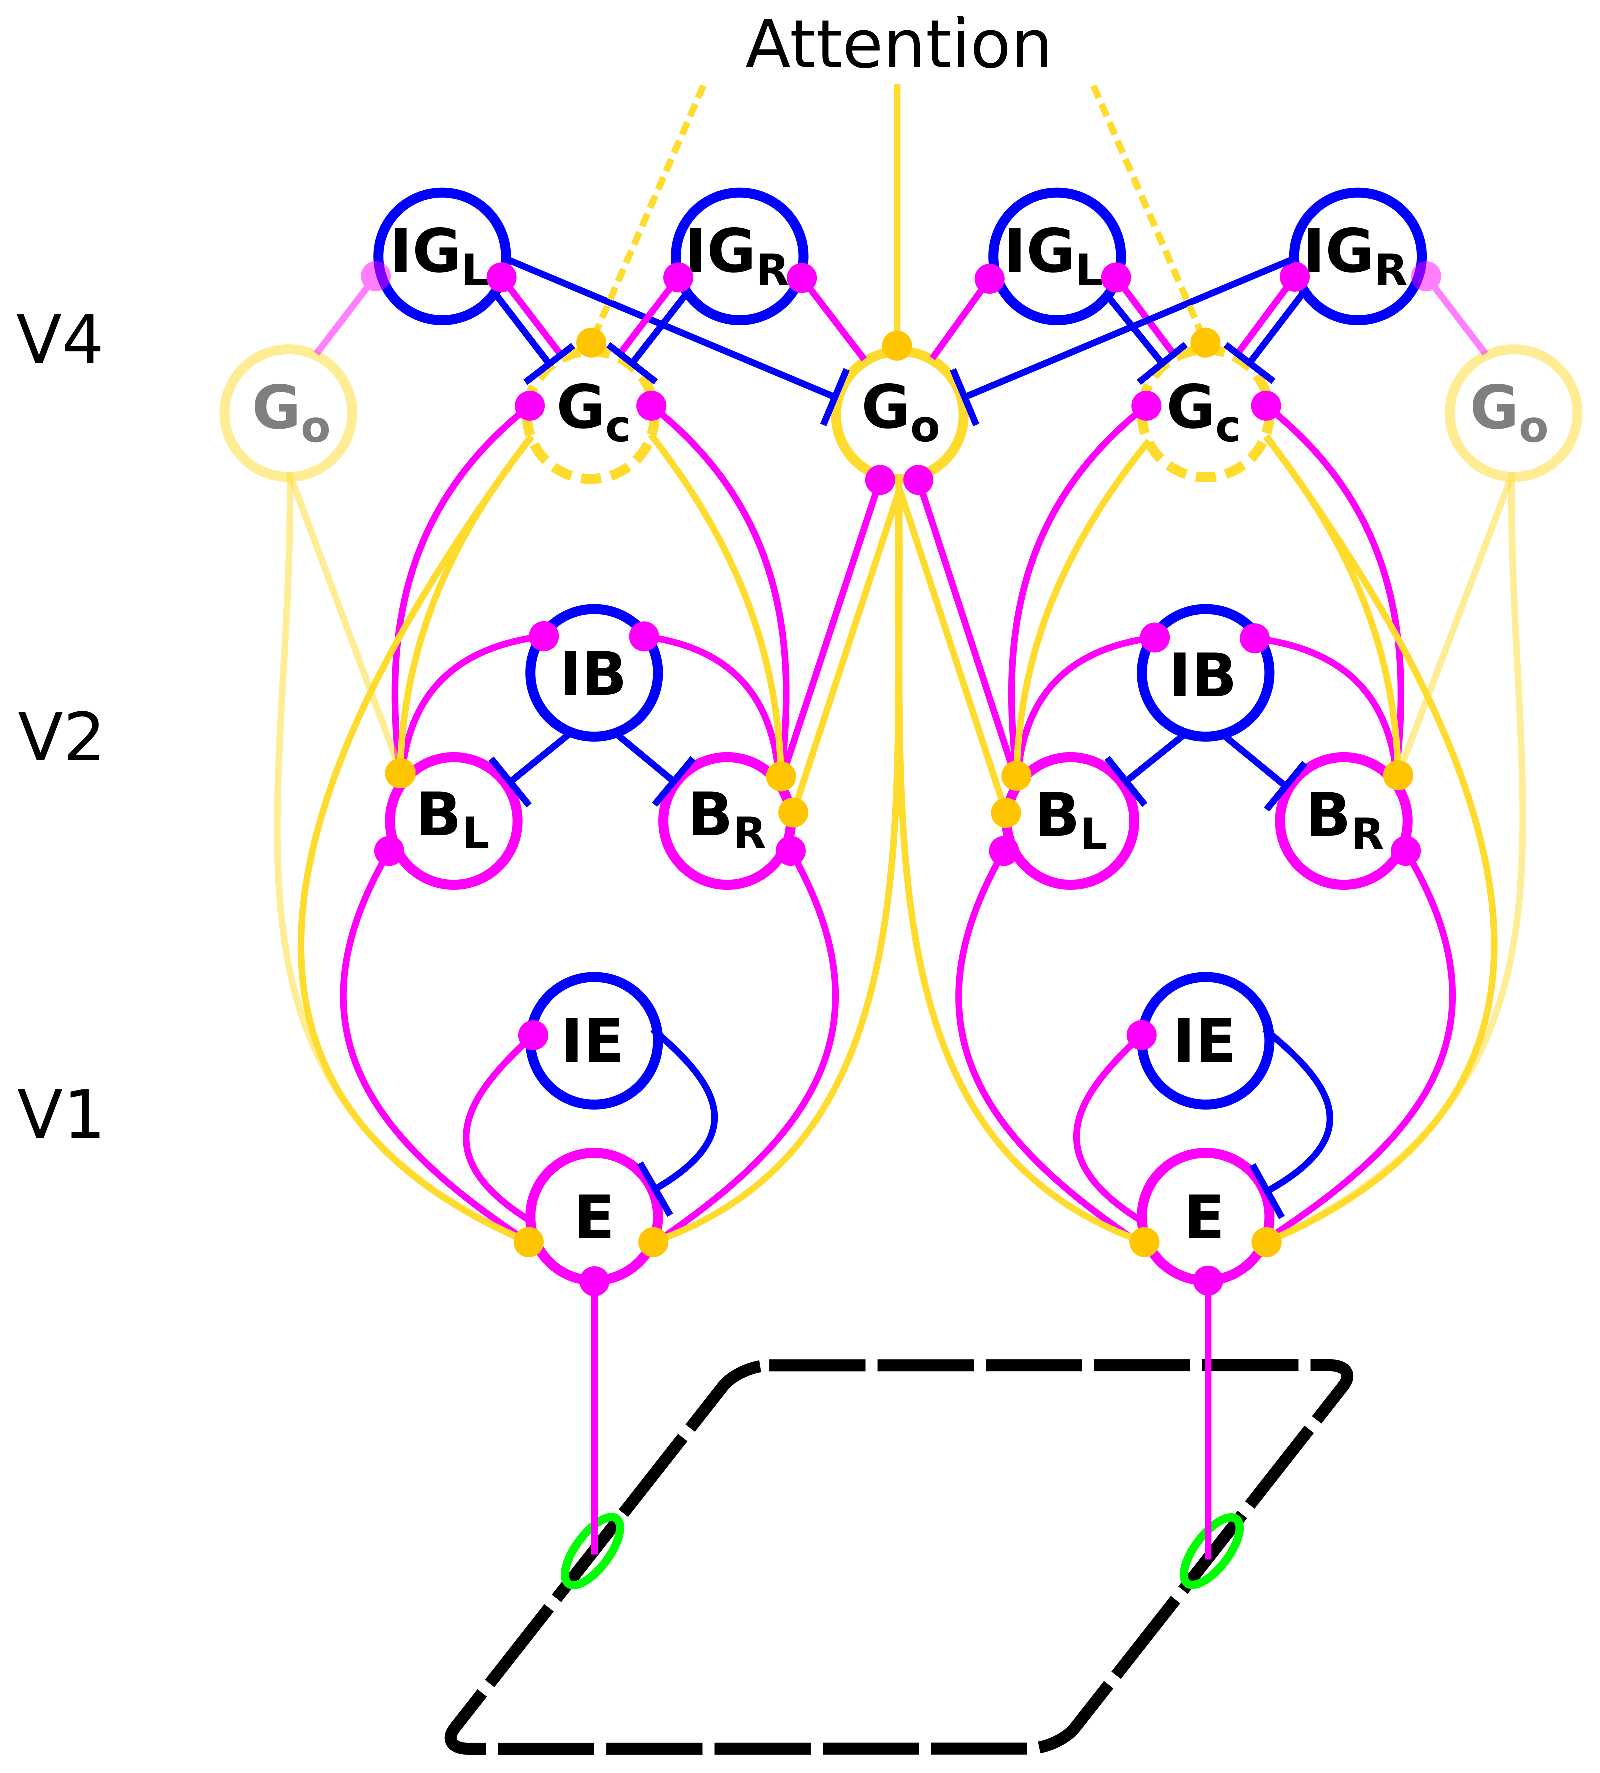
\includegraphics[width=0.75\textwidth]{Contour/figs/Fig1.eps}
\makeatletter
\let\@currsize\normalsize
% simplify caption
\caption[Structure of the grouping model network]{Structure of the model network. Each circle stands for a population of neurons with similar receptive fields and response properties. Magenta, blue, and orange lines represent feedforward excitatory, lateral inhibitory, and feedback excitatory projections, respectively. Top-down attention is modeled as input to the grouping cells and can therefore either be directed towards objects (solid lines) or contours (dashed lines) in the visual field (top).}
\label{Fig:anatomy}
\end{figure}

\begin{figure}[t]
\centering
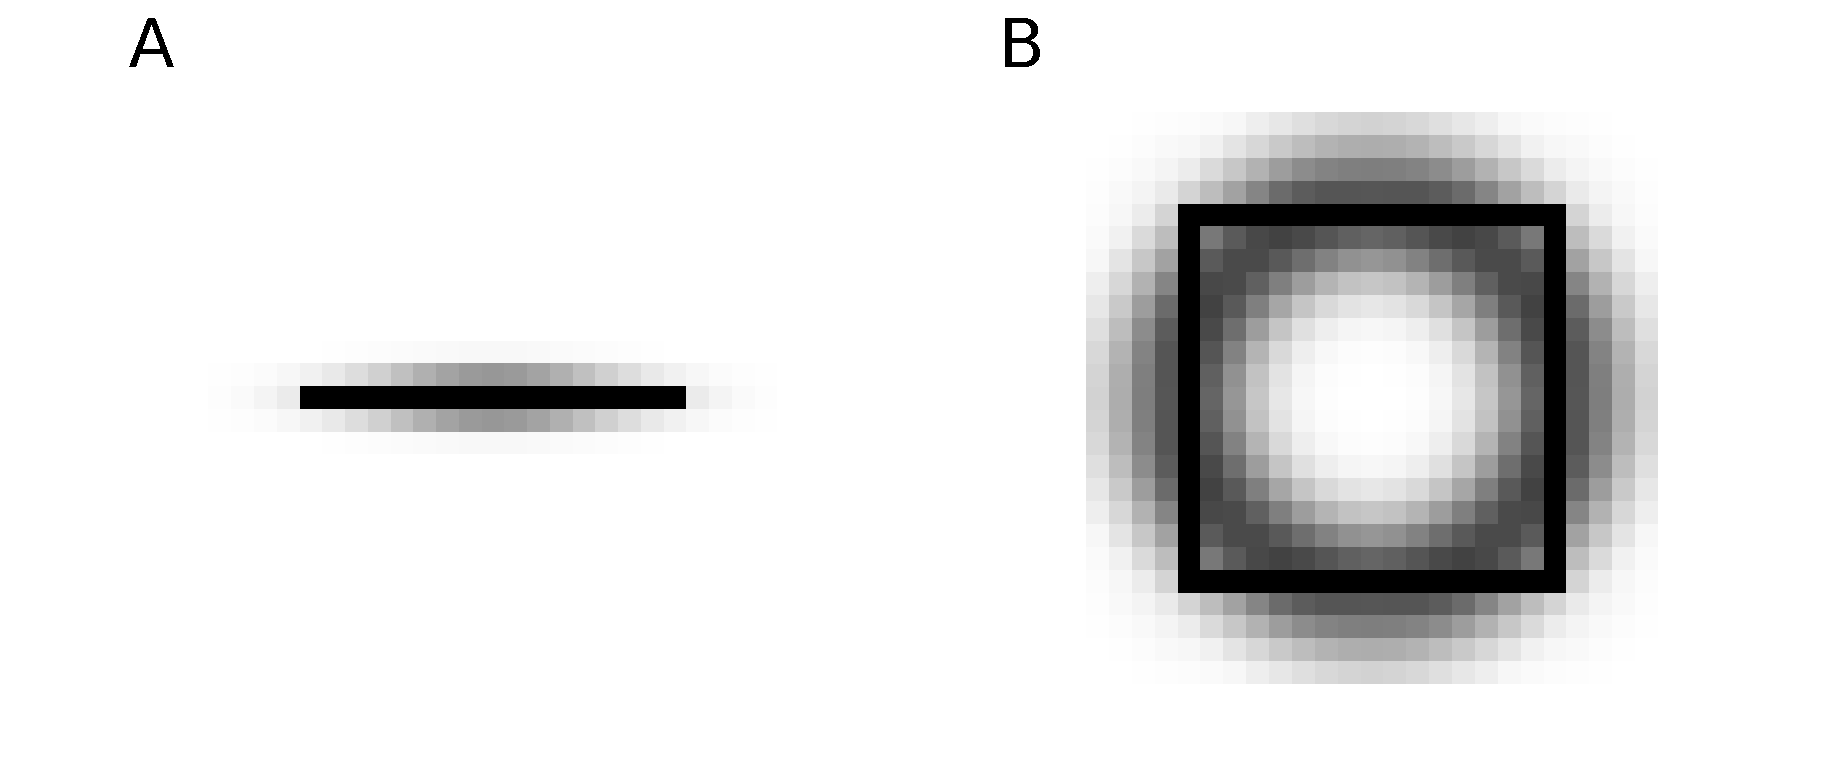
\includegraphics[width=\textwidth]{Contour/figs/Fig2.eps}
\makeatletter
\let\@currsize\normalsize
\caption[Contour and object grouping cell receptive fields]{Spatial distribution of border-ownership cell to grouping cell connectivity; darker pixels indicate stronger connection weights. A) Contour grouping neurons integrate features along oriented contours (horizontal line shown in black), emphasizing the Gestalt principle of good continuation. B) Object grouping neurons integrate features in a co-circular pattern (square figure shown in black), emphasizing the Gestalt principles of convexity and proximity.} 
\label{Fig:BG_projections}
\end{figure}

In V4, two different types of grouping cells exist. Contour grouping
cells ($\rm G_c$) integrate local edge information and are selective
for oriented contours (Figure~\ref{Fig:BG_projections}A). Object grouping cells ($\rm G_o$) are sensitive to roughly co-circular arrangements of edges, thus implementing Gestalt laws of good continuation, convexity of contour, and compact shape (Figure~\ref{Fig:BG_projections}B). Competition between separate contours and objects is carried out by a population of inhibitory (IG)
cells. Grouping ($\rm G_c$ and $\rm G_o$) cells project back reciprocally to those B cells from which they receive input, and also to the E cells that project to those B cells. This feedback enhances the
activity of E cells along contours and biases the competition between
B cells to correctly assign border ownership along object boundaries. Importantly, feedback connections are modulatory, rather than driving, such that the feedback does not modify activities of cells that do not receive sensory input. Biophysically, this can be achieved if the feedback projections employ glutamatergic synapses of the NMDA type \citep{Wagatsuma_etal16a}.

To model the effect of object-based attention, we assume that areas
higher than V4 provide additional excitatory input to those grouping cells whose activity represents the presence of objects or contours in the visual scene,  as shown in Figure~\ref{Fig:anatomy}. This attentional input is driving (as opposed to modulatory) but it is relatively weak; we select its strength as 7\% of that of the driving input to the sensory (E) cells. In one part of this study (section~\ref{sec:feedback}), we model the effect of a lesion in V4 that removes the feedback completely by setting the weight of feedback connections from V4 to lower areas to zero.

Our approach is an extension of the proto-object-based model of perceptual organization proposed by \cite{Mihalas_etal11b}. Different
from their approach, we include a new population of contour grouping
neurons (the $G_c$ cells) to explain recent results on cortico-cortical interactions during contour integration~\citep{Chen_etal14}. As a result, top-down attention in our model can either be directed to 
contours or to objects. Our model is also able to reproduce the time course of neural responses in different visual areas, while the \cite{Mihalas_etal11b} model only explains mean neural activities. In order to create more complex input stimuli, we also increased the number of model orientations from two to four. As a simplification to their model, we only include one scale of grouping neurons since we focus on mechanisms that do not require multiple scales.

\subsection{Model implementation}
\label{sec:implementation}

Model neuronal populations (usually referred to as ``neurons'' in the
following) are represented by their mean activity (rate coding).  The
activity is determined by a set of coupled, first-order nonlinear
ordinary differential equations which was solved in MATLAB (MathWorks,
Natick MA) using standard numerical integration methods.  The mean
firing rate is necessarily positive, therefore units are simple
zero-threshold, linear neurons which receive excitatory and inhibitory
current inputs with their dynamics described by,
\begin{equation}
\label{eq:1}
\tau f'(t) = -f + \left[ \sum W \right]_{+}
\end{equation}
where $f$ represents the neuron's activity level and $\tau$ its time
constant, chosen as $\tau$ = $10^{-2}$ s for all neurons. The sum is
over all $W$ which are the neuron's inputs,
$f'$ is the first derivative of $f$ with respect to
time, and $[\,]_{+}$ means half-wave rectification.

All simulations were performed on a 300-core CPU cluster running Rocks
6.2 (Sidewinder), a Linux distribution intended for high-performance
computing.  A total of 100 simulations were performed for each
experimental condition, and our results are based on the mean neural
activities averaged over these simulations with different randomly
selected stimulus noise patterns, see sections~\ref{sec:contour_exp}
and~\ref{sec:FGO}.

To constrain our model parameters, we used three sets of
neurophysiological data. The first comes from recent contour grouping
results~\citep{Chen_etal14}, and our model was able to largely
reproduce the magnitude and time course of contour integration at both
the V1 and V4 levels. The second comes from studies of border-ownership coding
\citep{Zhou_etal00} and we show that our model not only explains the
emergence of border ownership selectivity but also its approximate
time course as reported in that study. The third set of experimental data
constraining our model is from the study by \cite{Qiu_etal07} of the
interaction between border-ownership selectivity and selective
attention. In order to fit the model
parameters, we started from the parameters given by
\cite{Mihalas_etal11b}, and modified them to fit the larger body of
experimental results to include contour integration, border-ownership
selectivity, and attentional selection.

\begin{figure}[t]
\centering
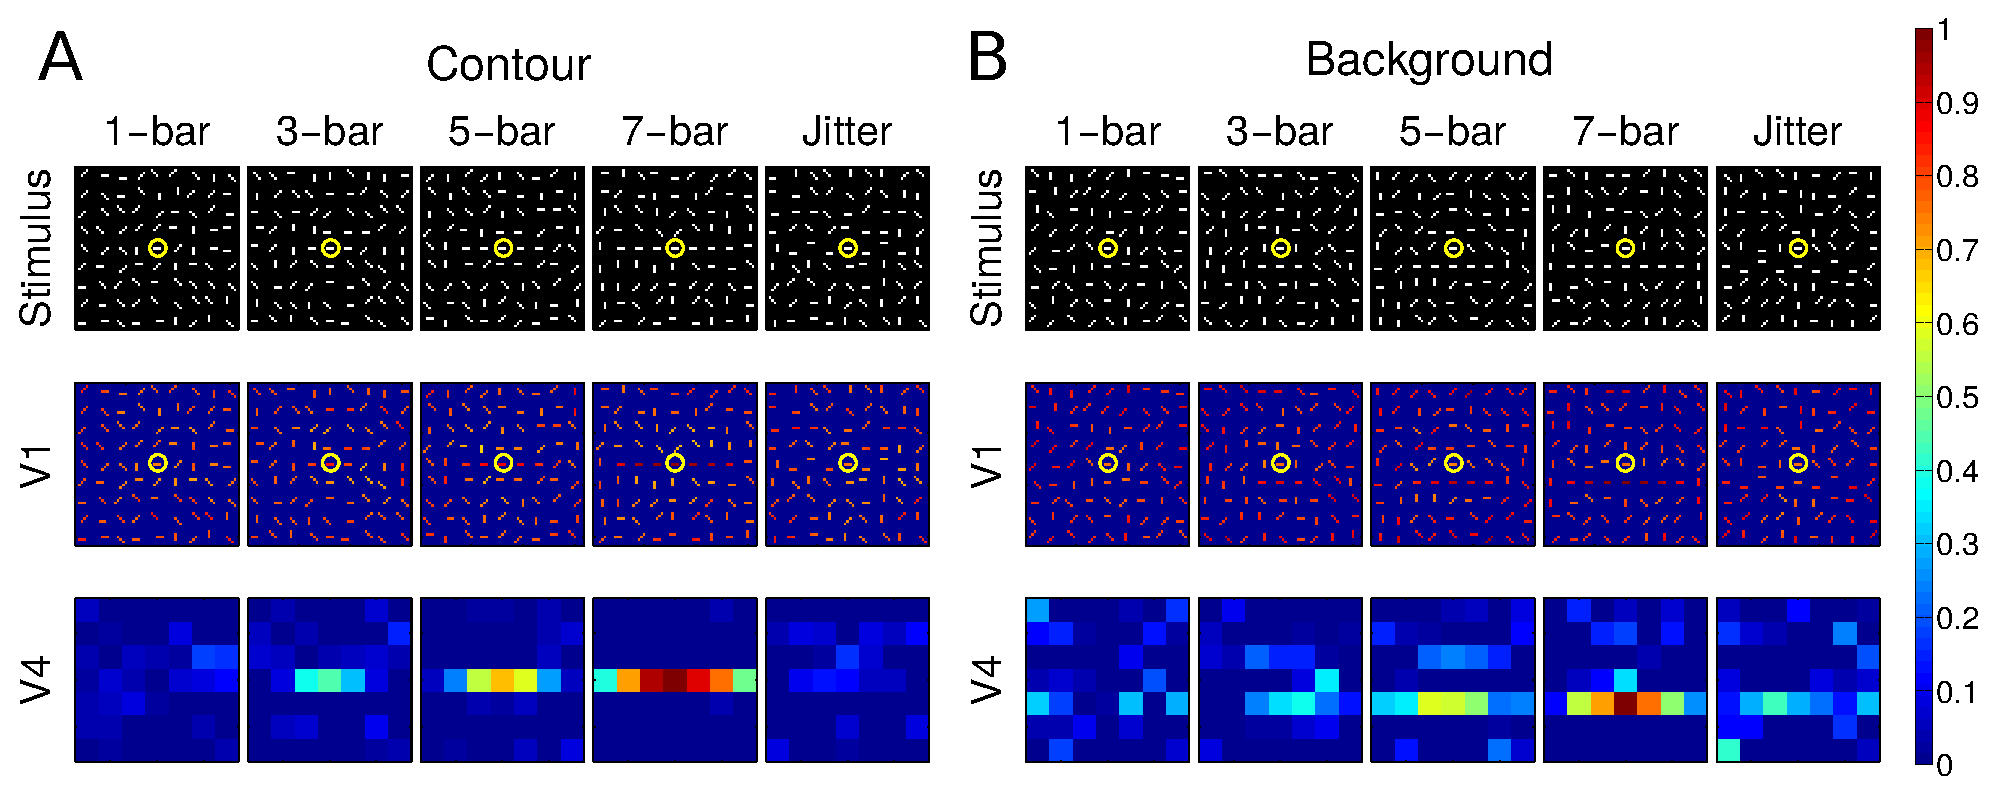
\includegraphics[width=\textwidth]{Contour/figs/Fig3.eps}
\makeatletter
\let\@currsize\normalsize
\caption[V1 and V4 population responses to contours]{Normalized V1 $E$ cell and V4 $G_c$ cell population responses to contours of varying lengths in either the contour (A) or the background (B) condition. In (A), the ``recorded'' neuron is on the contour; in (B), it is offset from the contour. The top row shows stimuli, the second and third rows show activity in model areas V1 and V4, respectively. Yellow circles mark the RFs of the V1 neurons whose activity is shown in Figure~\ref{Fig:Neural_responses}. Columns in each condition show, from left to right, increasing contour length, with the right-most column showing a jittered stimulus configuration (see text). Neural activity is color coded and normalized to the 7-bar stimulus in both contour and background conditions, with warmer colors representing higher activity (see color bar at right).}
\label{Fig:Contour_Results}
\end{figure}

\subsection{Contour integration experiments} 
\label{sec:contour_exp}

For the contour integration experiments reported by \cite{Chen_etal14}, awake behaving monkeys were trained to perform a two-alternative forced-choice task using two simultaneously presented patterns, one containing a contour embedded in noise and one that was noise only (see Figure~\ref{Fig:Contour_Results} for examples).  The patterns were composed of $0.25^{\circ}$ by $0.05^{\circ}$ bars distributed in $0.5^{\circ}$ by $0.5^{\circ}$ grids.  The diameter of the patterns was $4.5^{\circ}$, and the number of bars in the embedded contour was randomly set to 1, 3, 5, or 7 bars within a block of trials in order to control the saliency of the contour.  To obtain a reward, the monkey had to saccade to the pattern that contained the contour. When the number of bars was set to 1, both presented stimuli were noise patterns, and the monkey was rewarded randomly with a probability of 50\%.  While the animals were performing the task, simultaneous single- or multi-unit recordings were made in area V1 and V4 neurons with overlapping receptive fields.

We modeled these experiments by creating visual stimuli contained in a
$4.5^{\circ}$ by $4.5^{\circ}$ area. We ``recorded'' from the V1 receptive
field that was at the center of the stimulus (marked by the yellow circles in Figure~\ref{Fig:Contour_Results}), as well as from the
corresponding V4 neuron. Input from this area was projected onto a V1 layer of $64 \times 64$ neurons, each with a receptive field size of $\sim0.7^{\circ}$ so the receptive fields overlapped ten-fold at each location in the visual field.  We divided the input field into a $9 \times 9$ grid (each grid point at the center of a $0.5^{\circ}$ by $0.5^{\circ}$ area) and we placed at each grid location a stimulus bar 
consisting of three adjacent pixels, corresponding to a size $\sim0.21^{\circ}$ by $\sim0.07^{\circ}$. Each stimulus bar had one of four orientations, $0, \pi/4, \pi/2,$ or $3\pi/4$.  As in the \cite{Chen_etal14} experiment, contours consisted of 1, 3, 5, or 7 adjacent stimulus bars. We positioned the contour either at the center of the visual field so that the center element of the contour was in the RF of the ``recorded'' cell (Contour condition, Fig.~\ref{Fig:Contour_Results}A), or offset from the center of the
visual field, such that the ``recorded'' neuron was {\em next} to the
contour (Background condition, Fig.~\ref{Fig:Contour_Results}B). We changed the length of the contour by adding bars to both ends of the contour. Due to their size, V4 receptive fields basically enclosed the entire contour. For more details on the stimulus configuration, see Section~\ref{sec:contour}.

\subsection{Figure-ground segregation experiments} 
\label{sec:FGO}

For the figure-ground segregation experiments~\citep{Zhou_etal00,  Qiu_etal07, Zhang_vonderHeydt10}, awake, behaving monkeys were trained on a fixation task.  Receptive fields of each recorded neuron in areas V1 and V2 were first mapped to determine the optimal stimulus properties for that neuron. Afterwards, in some experiments, a square
shape was presented on a uniform gray background with one edge of the
square centered on the receptive field of the neuron at the neuron's
preferred orientation.  In other experiments (results shown in
Figure~\ref{Fig:Overlap_Square_exp_model}) %and~\ref{Fig:Overlap_Square})
the stimulus consisted of two partially
overlapping squares, and again the receptive field of the recorded
neuron was centered at its preferred orientation on one edge of one of
the squares.  The size of the square varied between experiments but it
was always chosen such that the closest corner was far away from the
classical receptive field of the recorded neuron. The square was
presented in two positions between which it was ``flipped'' along the
long axis of the neuron's receptive field. For instance, if the preferred orientation was vertical, the square was presented either to
the left or the right of the cell's receptive field (we used this
example in the choice of the indices in Figure~\ref{Fig:anatomy}).
The difference in the firing rate of the neuron for when the square
appears on one side versus the other side is defined
as the border-ownership signal. Importantly, in all stimulus conditions, local 
%bh are you sure you want to use the word "contents"? do you mean "context" instead in contrasting local vs. global?
contents 
%
within the receptive field of the neuron remained the same between these two conditions; only global context changed, so the neuron had to integrate information from outside its classical receptive field.

We modeled these experiments by creating visual stimuli that were projected onto the V1 layer. The input to the simulation was either a
single square of a size that maximally activated $\rm G_o$ grouping
cells of the size chosen in our model, or two partially overlapping
squares, as shown in Figure~\ref{Fig:Overlap_Square_exp_model}, with each of these squares having the same optimal size. In other models
\citep{Craft_etal07,Mihalas_etal11b,Russell_etal14}, grouping cells of
many scales are present, covering the range of possible objects in the
input. We calculated border-ownership selectivity at the V2 level
using the vector modulation index defined in section~\ref{sec:vmi}.
In order to create noisy versions of the single square image (Figure~\ref{Fig:Square_Noise}), we followed a similar approach as in
the contour integration experiments, section~\ref{sec:contour_exp}.
We again divided the visual field into a $9 \times 9$ grid and we positioned horizontal and vertical bars at specific grid points to
generate a square. We then placed a stimulus bar at all other grid
points, with their orientations randomly chosen from four possibilities, $0, \pi/4, \pi/2,$ and $3\pi/4$.

\subsection{Quantitative assessment of border-ownership selectivity:
  vector modulation index}
\label{sec:vmi}

While the border ownership signal discussed in the previous section (the difference in firing rates between presentations of a figure on the two sides of a a neuron's RF) is useful to characterize border-ownership selectivity for that particular neuron, description of population behavior requires a more general measure. We use the vector modulation index, introduced by \cite{Craft_etal07} and defined
by the expression 
\begin{equation}
\label{eq:2}
\overrightarrow{\mathbf{v}}(x,y) = m_{\hat{\imath}}(x,y)\hat{\imath} + m_{\hat{\jmath}}(x,y)\hat{\jmath}
\end{equation}
where $\hat{\imath}$ and $\hat{\jmath}$ are unit vectors along the horizontal and vertical image axis, respectively, and the components $m_{\hat{\imath}}(x,y)$ and $m_{\hat{\jmath}}(x,y)$ are the usual modulation indices along their respective axes, defined as
\begin{equation}
\label{eq:3}
\begin{split}
	m_{\hat{\imath}}(x,y) = \frac{\sum_{\theta}
        B_{\theta}(x,y)\cos\theta}{\sum_{\theta}
                \left|B_{\theta}(x,y)\cos\theta\right|} \\
	m_{\hat{\jmath}}(x,y) = \frac{\sum_{\theta}
        B_{\theta}(x,y)\sin\theta}{\sum_{\theta}
                \left|B_{\theta}(x,y)\sin\theta\right|}
\end{split}
\end{equation}
Here, $B_{\theta}(x,y)$ is the border ownership signal (difference between the activities of the two opposing B neurons) at the preferred
orientation $\theta$ at position $(x,y)$, and $\theta$ runs over all
angles taken into account in the model (four directed orientations in our case, namely $0, \pi/4, \pi/2,$ and $3\pi/4$, each with both side-of-figure preferences). Vertical bars in the sums in the denominators indicate absolute values.

Both components in Eq.~\ref{eq:3} are limited to values between +1 and
-1. For the x-component, for instance, a positive value of
$m_{\hat{\imath}}(x,y)$ signifies that the figure is to the right of
position (x,y) and a negative value signifies that the figure is to
the left. Its absolute value indicates the ``strength'' of the
border-ownership signal, with zero being equivalent to ambivalence
between left and right. Corresponding comments apply to the y-component, $m_{\hat{\jmath}}(x,y)$, regarding the figure's position
upward or downward of (x,y). The direction of the vectorial modulation
index $\overrightarrow{\mathbf{v}}(x,y)$ defined in Eq.~\ref{eq:2} indicates the position of the foreground figure in the two-dimensional image plane relative to the point (x,y). For instance, positive values in both components [$m_{\hat{\imath}}(x,y) > 0$, $m_{\hat{\jmath}}(x,y) > 0$] indicate that the figure is located upwards and to the right of (x,y).

\section{Results}
\label{sec:results}

\subsection{Contour enhancement in V1 and V4}
\label{sec:contour}
We examined contour-related responses in our model using visual stimuli composed of collinear bars among randomly oriented bars (Figure~\ref{Fig:Contour_Results}), closely matching the stimuli used
in the physiological experiments by \cite{Chen_etal14}. The number of
collinear bars constituting an embedded contour was set to either 1, 3, 5, or 7 bars, determining the length of the embedded contour, which also controlled its saliency.  When the number of collinear bars was one, the stimulus was identical to a noise pattern. We compared the
activity of model neurons whose RFs are centered on the contours or in
the noise background (but close to contours) with that obtained in the
analogous positions during neurophysiological recordings.

V1 responses were split into those of neurons on contour sites (C-sites) and background sites (B-sites). For contour sites (Figure~\ref{Fig:Contour_Results}A), the embedded contour was centered
on the RF of a neuron with a preferred orientation matching that of
the contour. For background sites, the contour was laterally placed
0.5$^{\circ}$ away from the RF center of the recorded neuron, and a
background bar was placed in the RF (Figure~\ref{Fig:Contour_Results}B), with the contour orientation again matching the preferred orientation of the recorded neuron. Both V1 and V4 neurons along the contour showed increased activity with contour length. Neurons on the background showed increased suppression with contour length. Correspondingly, we show in Figure~\ref{Fig:Neural_responses} the responses of neurons whose preferred orientations align with the contours (yellow circles in Figure~\ref{Fig:Contour_Results}).

\begin{figure}[t!]
\centering
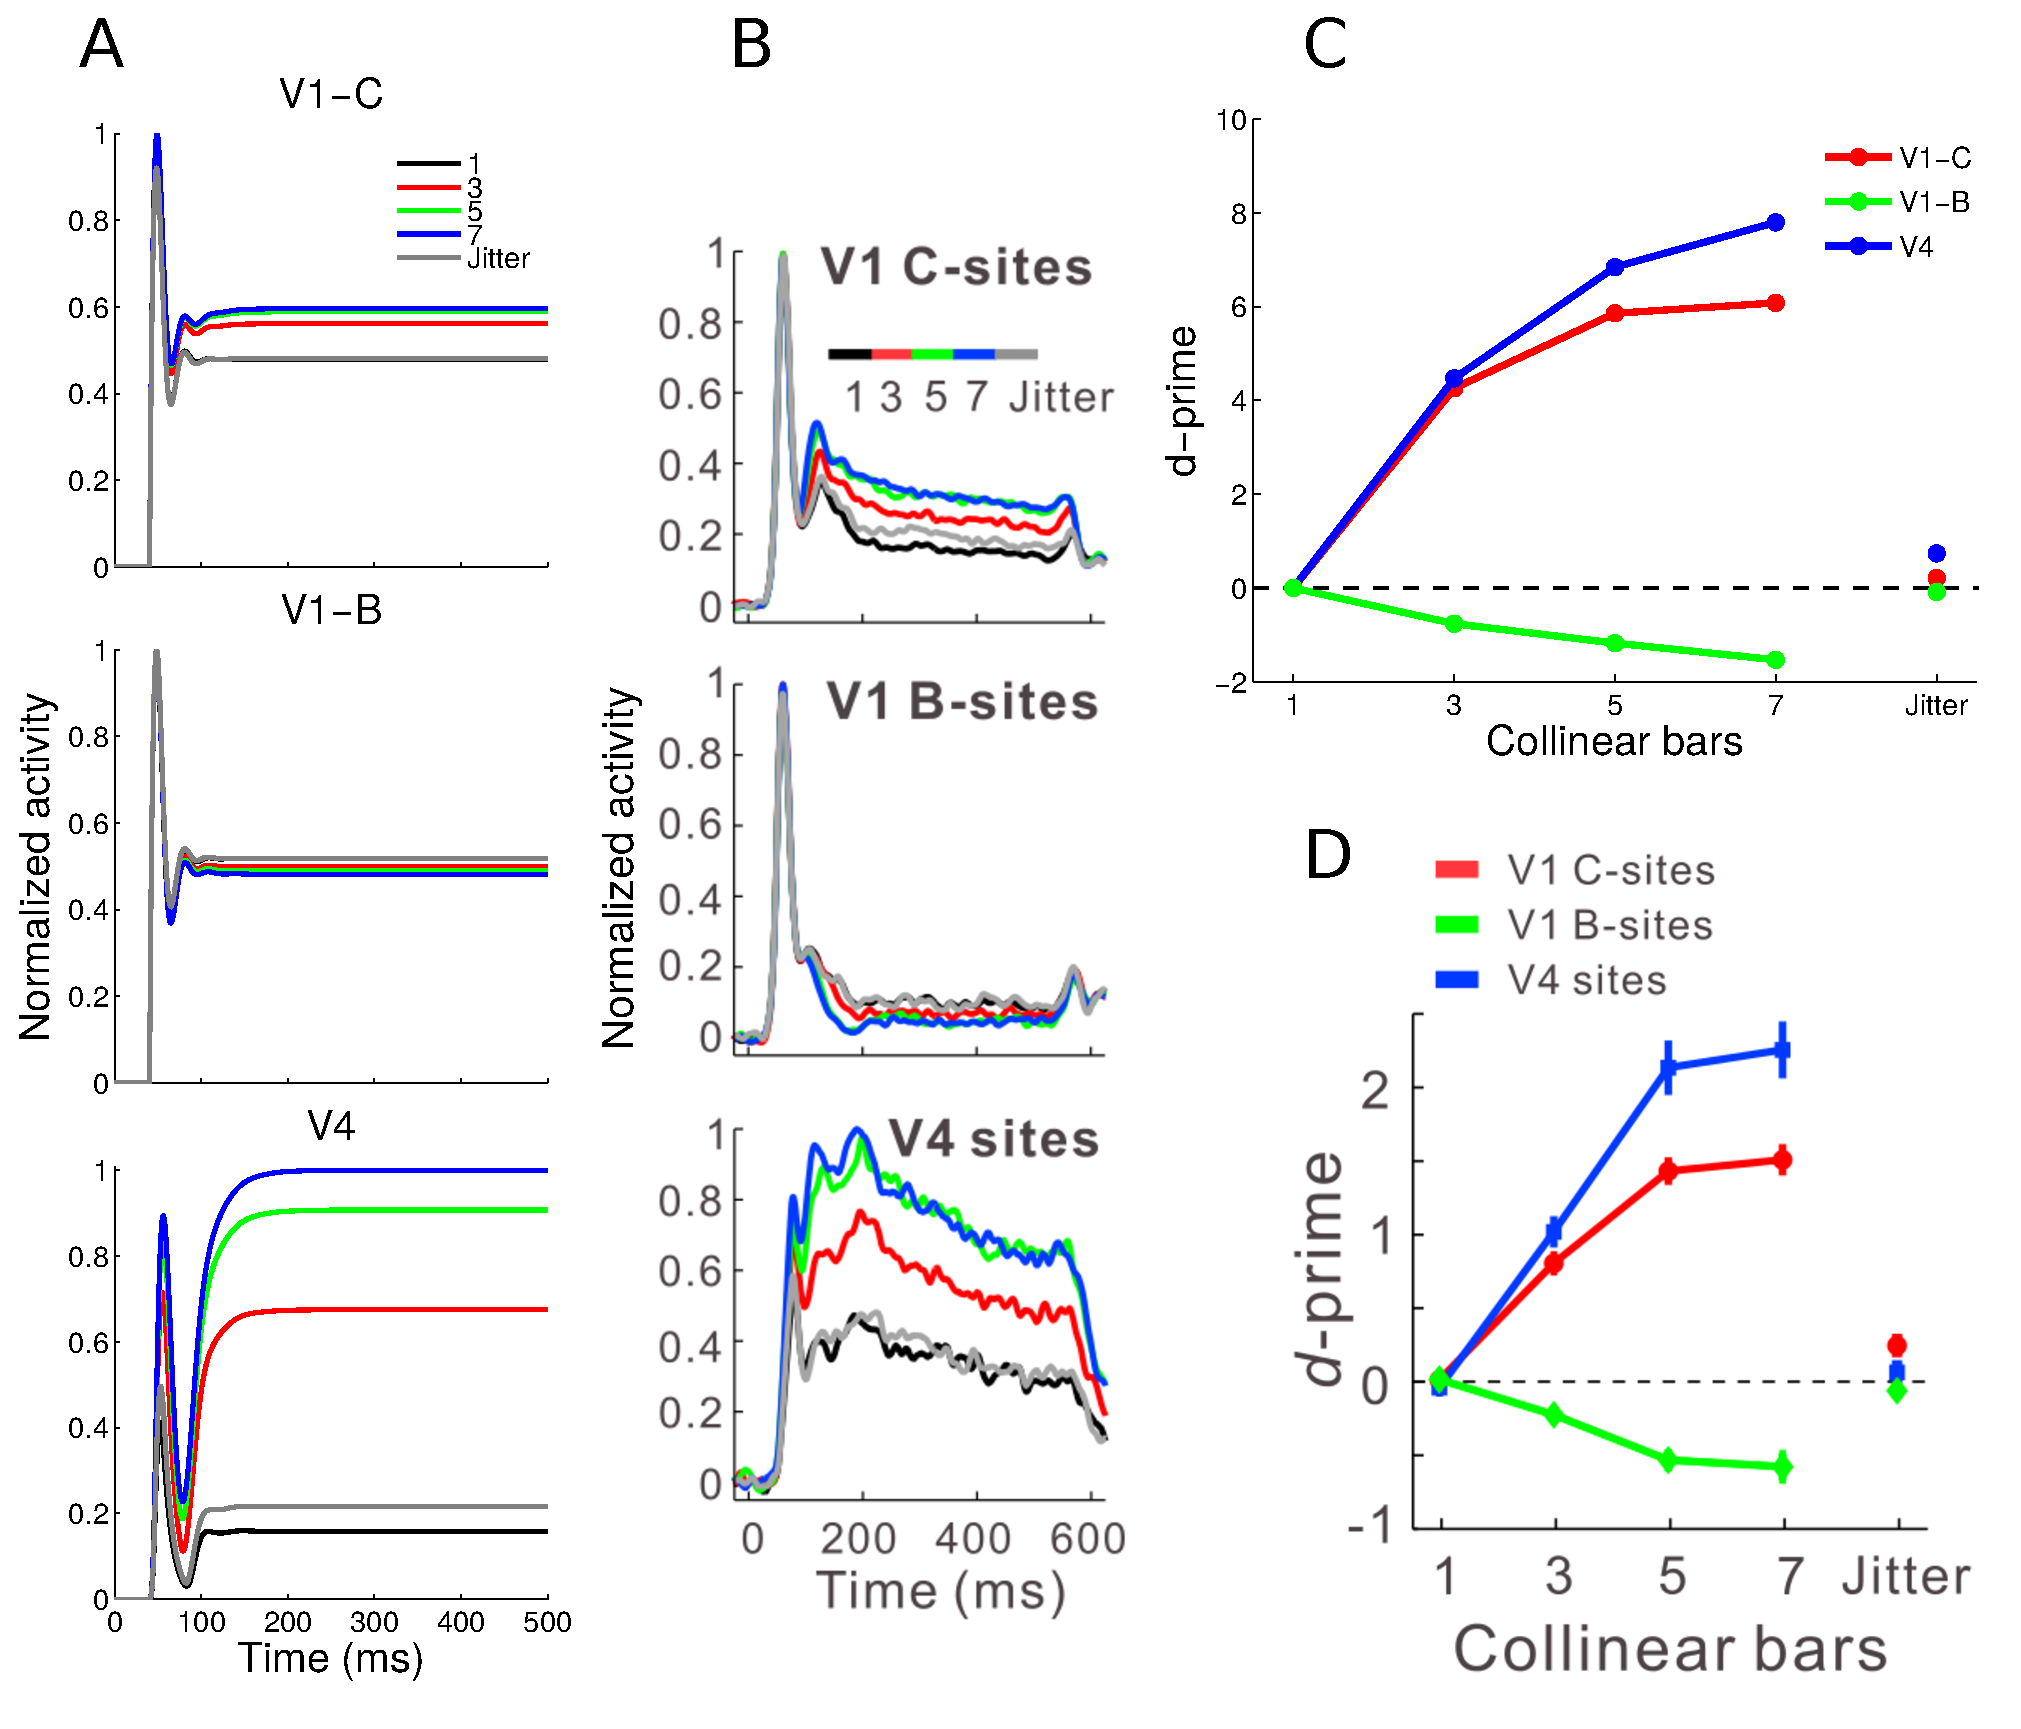
\includegraphics[width=0.75\textwidth]{Contour/figs/Fig4.eps}
\makeatletter
\let\@currsize\normalsize
\caption[Time course of neural activity in V1 and V4 and the contour-response d-prime measure]{Normalized V1 $E$ cell (contour and background sites) and V4 $G_c$ cell neuronal activity and contour-response $d'$ to contours of varying lengths. (A) V1 contour (top) and background (middle) sites and V4 sites (bottom).
%showed facilitation followed by saturation with increasing contour length (see legend). V1 background sites showed greater suppression with longer contours. 
The jitter condition involved a 7-bar pattern where each bar was laterally offset to disrupt collinearity. (B) Corresponding experimental observations showing normalized and averaged PSTHs from the~\cite{Chen_etal14} study. (C) Contour-response $d'$ was higher for the V4 sites compared to the V1 contour sites.
%, and was facilitated by  increasing contour length. 
V1 background sites had increasingly  negative $d'$ with longer contours.
%, indicating background suppression. The jitter condition reduced the absolute value of the $d'$ values to close to zero, making it similar to the baseline noise condition.
(D) Corresponding experimental observations, showing the mean contour-response $d'$ from the~\cite{Chen_etal14} study. Panels B and D are modified from Figure~2 of~\cite{Chen_etal14}. All model results (neural responses and contour-response $d'$) are averages for a single neuron over 100 simulations.}
\label{Fig:Neural_responses}
\end{figure}

Except for an input delay of 40ms corresponding to the duration of visual processing from the retina to V1, we did not add any time delays in the feedforward or feedback connections of our model, as we were not attempting to reproduce any specific latency effects. Nevertheless, our model generally reproduced the dynamics of neural responses to contours in both V1 and V4 observed in the \cite{Chen_etal14} experiment (Figure~\ref{Fig:Neural_responses}A). The most salient feature of the neuronal responses is that the levels of sustained activity differ based on the number of bars in the embedded contour. This is observed both for contour sites and for background sites but, importantly, this effect went in opposite directions for these two cases.  As the number of collinear bars increased from one to seven, V1 contour sites centered on the contour showed increased activity, with response saturation after five bars. In contrast, V1 background sites that were offset from the embedded contour showed a decrease in activity with increasing number of bars in the background (response suppression). Similar to V1 contour sites, V4 sites showed saturating responses with increasing contour lengths (Figure~\ref{Fig:Neural_responses}A, bottom). These results were qualitatively similar to those obtained in
the~\cite{Chen_etal14} experiments which are reproduced in
Figure~\ref{Fig:Neural_responses}B (their Figure~2A).

The model data also showed strong onset transients in both (contour
and background) V1 populations (Figure~\ref{Fig:Neural_responses}A,
top and center), again in good agreement with experimental results
(Figure~\ref{Fig:Neural_responses}B, top and center). Transients in V4
neurons were weaker, in both model and experimental data, and nearly
absent in the experimental data (though not the model) for longer contours (Figure~\ref{Fig:Neural_responses}B, bottom). The transient peak observed in the model results is due to a sharp suppression of the activity level for a short ($<50$ms) period which is not observed in the empirical data. We believe that this suppression is due to the  strong inhibition at the V4 level between G and IG cells, without equivalent excitation between different G cells.

Following \cite{Chen_etal14}, we quantitatively analyzed the contour responses using the d-prime $(d')$ metric from signal detection theory~\citep{Green_Swets66}, which quantifies the difference in distributions of mean neuronal firing rates between a contour pattern and the noise pattern integrated over the whole interval shown in Figure~\ref{Fig:Neural_responses}A,B, \ie 0-500 ms.  Neuronal responses to the 1-bar pattern (the noise pattern) were the baseline for examining contour-related responses in V1 and V4, this pattern therefore had a contour-response $d'$ of zero. The contour-response $d'$ increased with contour length for both the V1 contour and V4 sites, and $d'$ decreased with contour length for the V1 background sites, Figure~\ref{Fig:Neural_responses}C.

The agreement between model (Figure~\ref{Fig:Neural_responses}C) and
experimental results (Figure~\ref{Fig:Neural_responses}D) is striking.
One difference we note is that the absolute values of all model $d'$
substantially exceed the corresponding experimental values. This is to be expected since no noise was included in the model (other than the random orientation of input stimulus bars which is also present in the experimental approach) while there are surely multiple sources of noise in the biological system. We have not thoroughly investigated this question but it is highly likely that addition of noise to the model will decrease the $d'$ values.

At first sight, it seems possible that V4 neurons respond with a higher firing rate to longer contours than to shorter ones simply as a consequence of the large size of RFs in V4. In this view, the enhanced responses in V4 with increasing contour length is due to the spatial summation of many bars within the RF at the optimal orientation, independent of their precise location in the RF. To investigate this possiblity, ~\cite{Chen_etal14} introduced a ``jitter'' condition to the 7-bar contour, where alternating collinear bars were laterally offset by a small amount (much less than the receptive field size) in order to disrupt the collinearity of the original contour. They showed that jittering disrupted the contour integration process and reduced the neural responses in V1 and V4 close to baseline levels (Figure~\ref{Fig:Neural_responses}B, gray lines). We found the same result in our model, Figure~\ref{Fig:Neural_responses}A, gray lines.  Furthermore, in the jitter condition, contour-response $d'$ approached baseline for the V1 and V4 sites, as shown in the rightmost points for
Figure~\ref{Fig:Neural_responses}D for experimental data and
Figure~\ref{Fig:Neural_responses}C for model results. In both cases,
no substantial difference between the jitter condition and the
baseline noise condition was observed.

We also investigated the orientation and position dependence of contour-related responses in V1 and V4, and found close agreement of
our model results with experimental data~\citep{Chen_etal14}. Due to space constraints, these results are presented in \hyperref[sec:appendix_fig]{Appendix A}.
%Supplementary Material. The results for V4 are presented in Supplementary Figure~\ref{Fig:V4_total} and the results for V1 are presented in Supplementary Figure~\ref{Fig:V1_total}.

\begin{figure}[t]
\centering
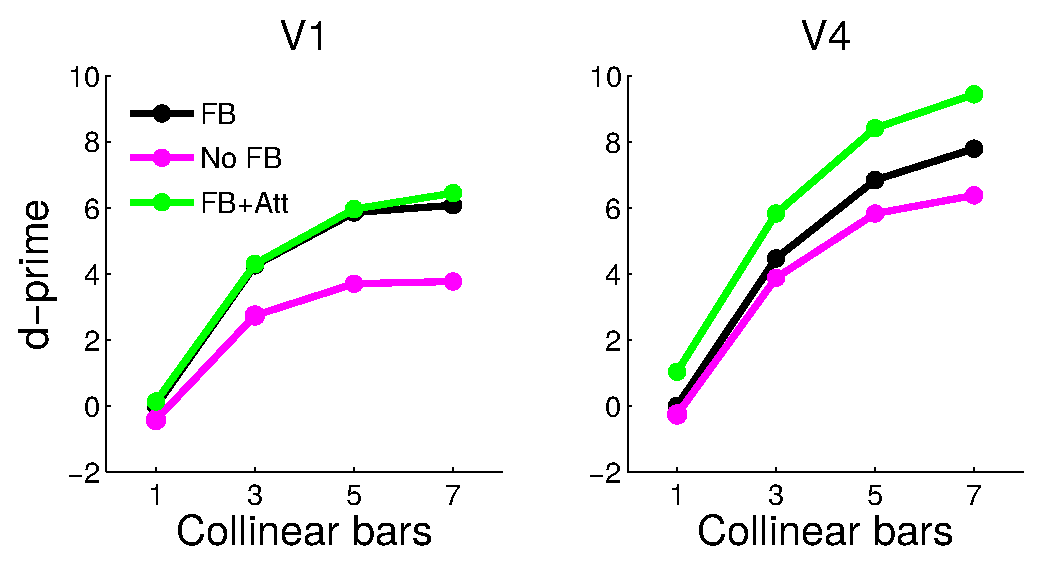
\includegraphics[width=\textwidth]{Contour/figs/Fig5.eps}
\makeatletter
\let\@currsize\normalsize
\caption[Model prediction of the effect of feedback and attention on contour-response d-prime]{Contour-response $d'$ in V1 $E$ cells (A) and V4 $G_c$ cells (B) for the model with (green) and without attention (black), and for the model with feedback removed (magenta). Attention strongly increased
contour-response $d'$ in V4 (B), while the lack of feedback strongly
decreased contour-response $d'$ in V1 (A).}
\label{Fig:FB_att}
\end{figure}

\subsection{The role of feedback and attention in contour grouping}   
\label{sec:feedback}
While different forms of attention exist that can be flexibly used for
different tasks, we choose here to focus only on the mechanisms of
object-based attention \citep{Egly_etal94,Scholl01,Kimchi_etal07,Ho_Yeh09}. We postulate that attention to objects acts at the level of grouping neurons, in
agreement with the \cite{Mihalas_etal11b} model.  As shown in that
study, modulation of the activity of grouping cells bypasses the need
for attentional control circuitry to have access to detailed object
features.  Instead, grouping neurons are used as ``handles'' of the
associated objects and it is in their interaction with feature-coding
neurons that features are assigned to objects. One of the consequences
of this mechanism is that the spatial resolution of attentional
selection is coarser than visual resolution since the smallest ``unit'' of spatial attentional deployment is the size of the receptive (and projective) field of grouping cells, which is considerably larger than the receptive fields of feature-coding neurons at the same eccentricity. Behavioral results show strong evidence in favor of this coarse attentional resolution~\citep{Intriligator_Cavanagh01}.

In our model, attention can be directed to objects, including contours. For the contour integration experiments, this is implemented as a top-down input to all contour grouping neurons at the attended location, but, importantly, 
%bh reads a little awkwardly, how about adding this?
there was
%
no direct input to the feature-coding edge (E) cells. As we have seen before (Figure~\ref{Fig:Neural_responses}), $d'$ in V1 and V4 populations increases with the number of collinear bars, even in the absence of attention.  In addition, we now show that attention increases the contour-response $d'$ for both V1 and V4 neurons, with
the additive effect being much larger in V4 than in V1 (Figure~\ref{Fig:FB_att}). For the 7-bar contours, attention increases
the contour-response $d'$ in V1 from 6.08 to 6.66 and in V4 from 7.80
to 11.59. This is consistent with findings that attention has a much
larger effect on higher-level neurons compared to early sensory
neurons~\citep[review:][]{Treue01}.

One of the advantages of computational modeling is that it allows the
study of scenarios that are difficult to implement empirically. One question that is difficult to answer experimentally is how removal of
feedback from V4 to lower visual areas would change neuronal responses in V1 and V4, structures that are known to be connected bidirectionally
\citep{Zeki78b,Ungerleider_etal07}. While it is possible to study the influence of feedback on V2 (and other areas) by cooling \citep{Hupe_etal98} or pharmacological inactivation~\citep{Jansen-Amorim_etal12} of area V4, such manipulations only allow limited control of the effect on multiple brain structures. In contrast, a computational model allows the study of interactions between different areas with perfect control. In the model,  we can eliminate all feedback from area V4 simply by ``lesioning'' the connections from the grouping neurons to the V2 and V1 neurons (setting their strength to zero), thus turning the model into a feedforward network.  We found that this has the opposite effect of applying attention on the $d'$ metric: the decrease in contour
response $d'$ was much larger in V1 compared to V4. Removing feedback
reduced the 7-bar contour-response $d'$ in V1 from 6.08 to 3.77, and
in V4 from 7.80 to 6.38 (Fig.~\ref{Fig:FB_att}). We note that the
contour-response $d'$ in V1 is above zero even without feedback from
grouping neurons because of the contribution of local excitatory
connections to contour integration.  This asymmetric effect in contour
response $d'$ in the two areas (V1 and V4) may point to the different
roles of feedforward and feedback processing in early vision. We are
not aware of any experimental manipulations that completely remove
feedback from area V4 without changing the circuitry in other ways, so
our results are a prediction awaiting experimental falsification.

\begin{figure}[t!]
\centering
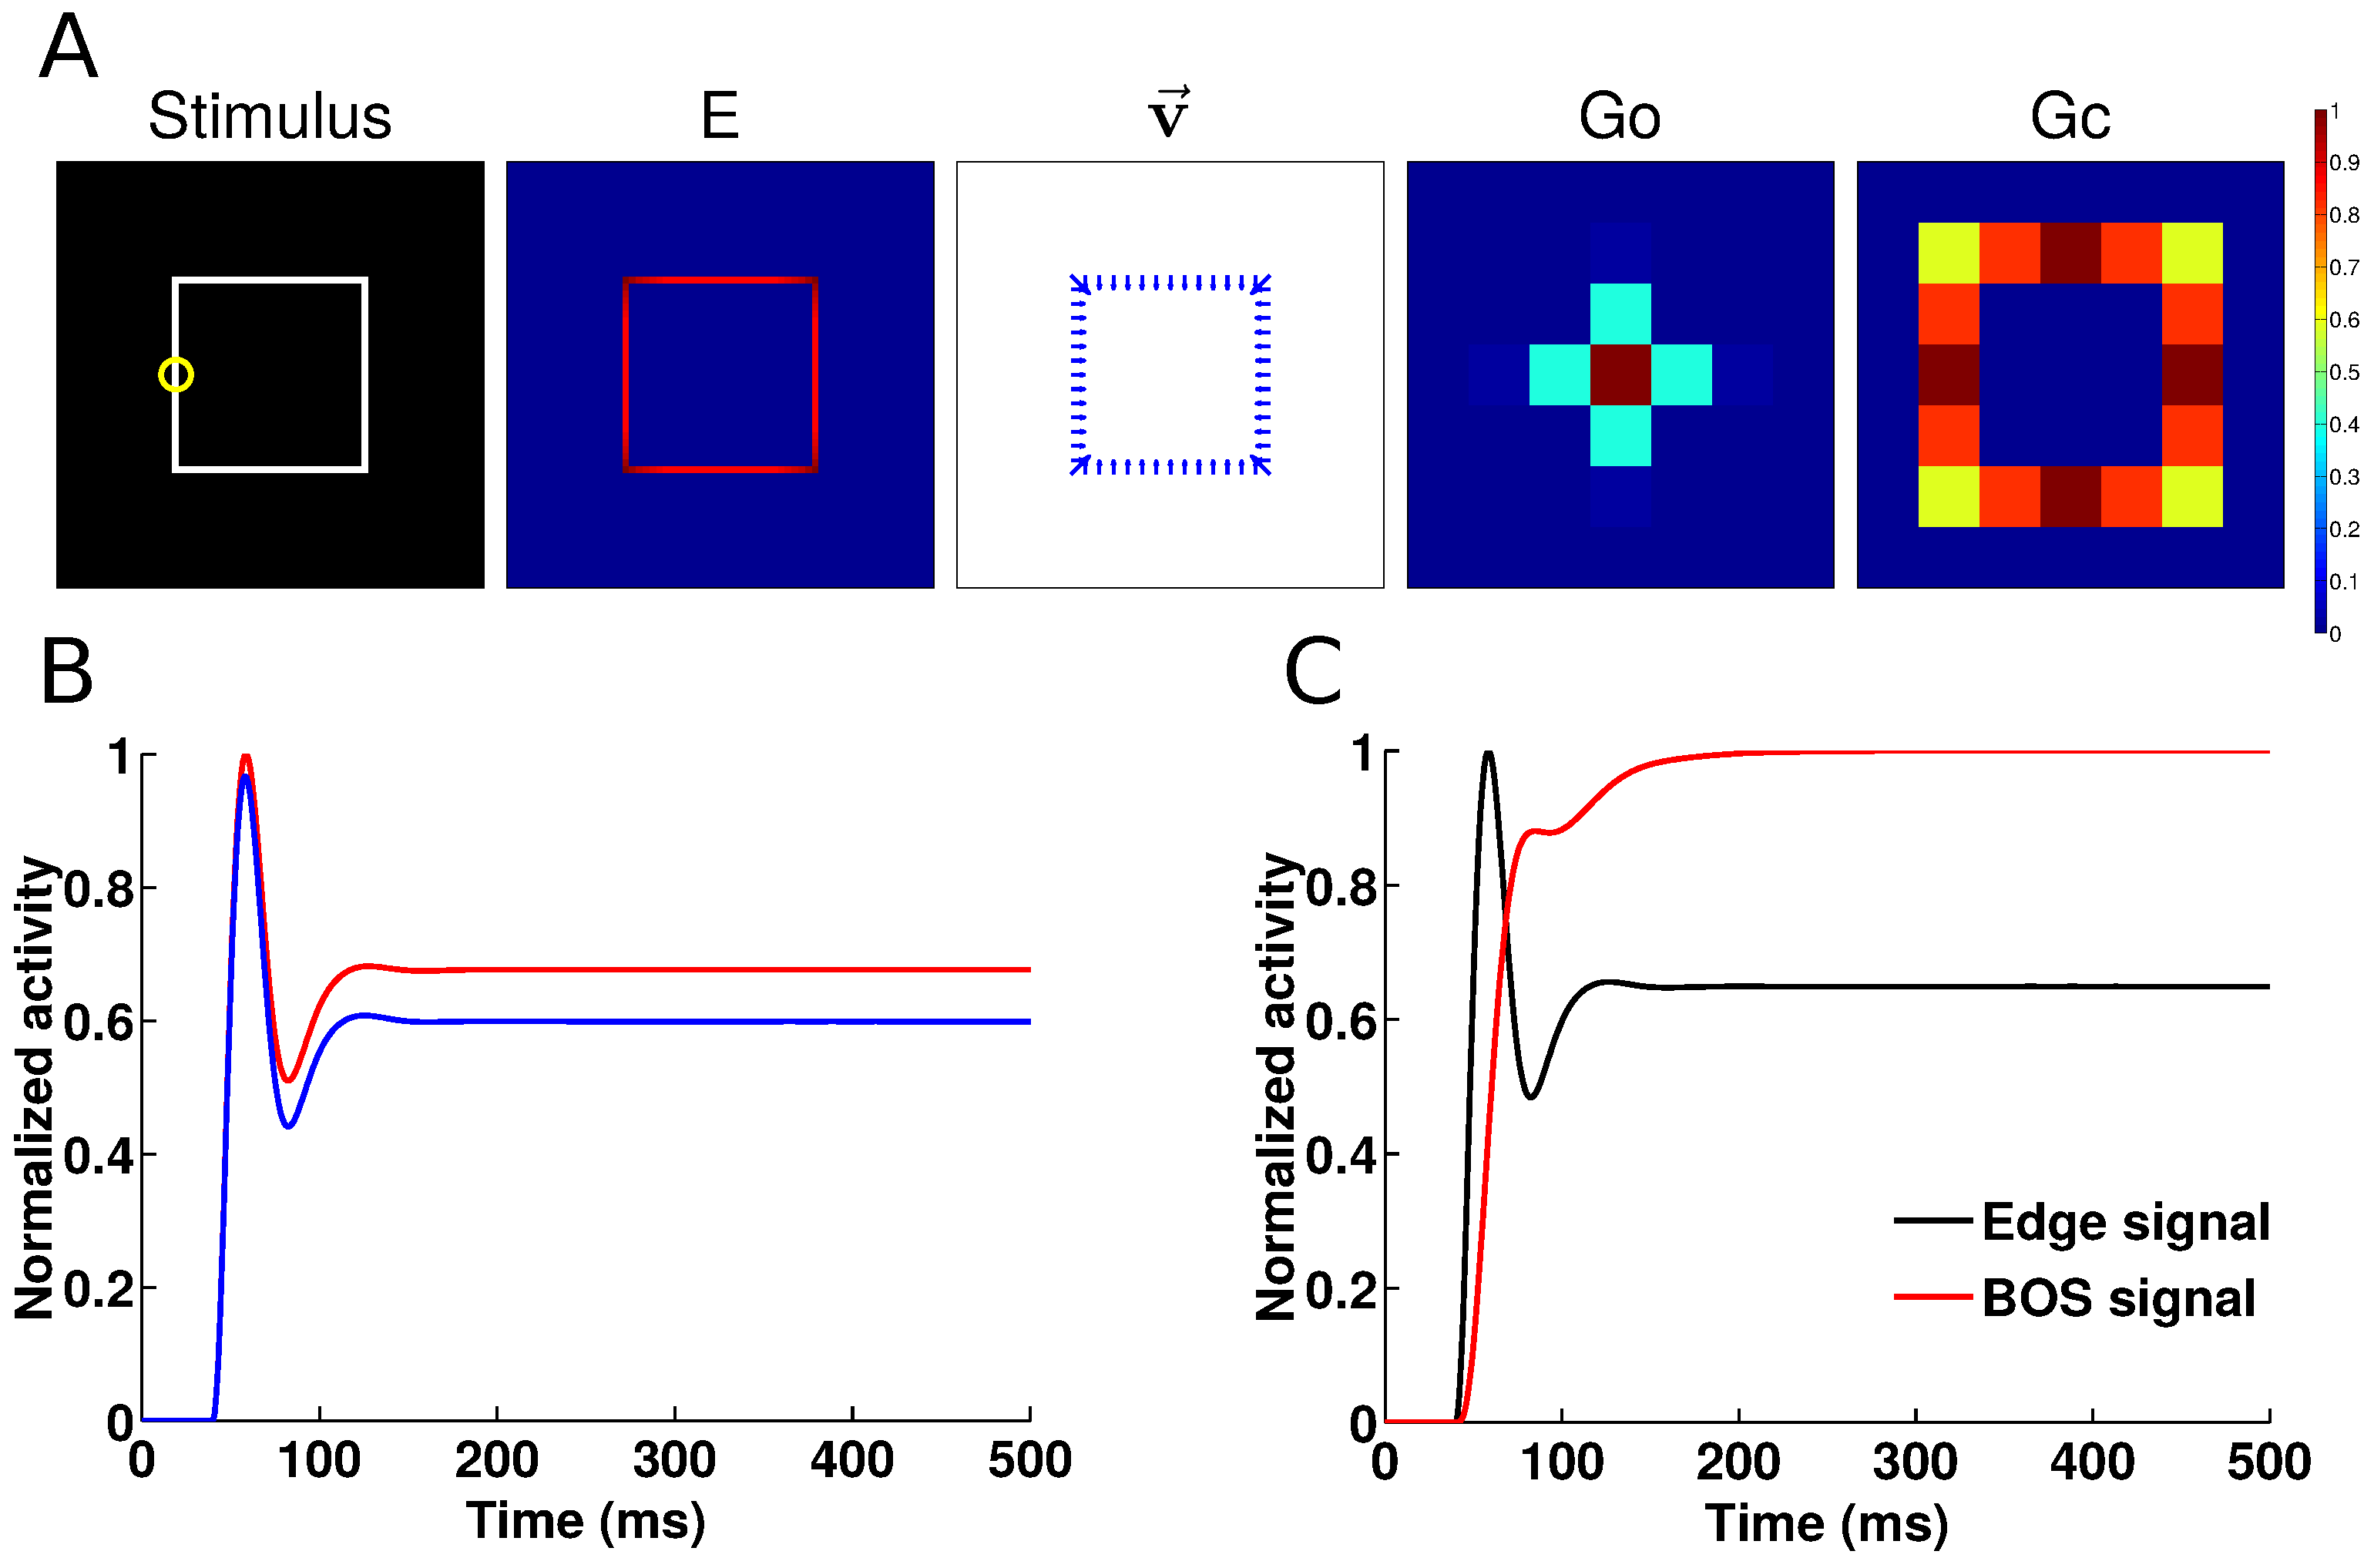
\includegraphics[width=\textwidth]{Contour/figs/Fig6.eps}
\makeatletter
\let\@currsize\normalsize
\caption[Time course of figure-ground segregation]{Figure-ground segregation of a square object as in the~\citet{Zhou_etal00} experiments. (A) Shown left to right are the input stimulus, the edge cell activity (E), the border ownership assignment along edges (shown as the vector modulation index $\protect\overrightarrow{\mathbf{v}}$, section~\ref{sec:vmi}), the object grouping neuron activity $(G_o)$ and the contour grouping activity $(G_c)$. Activities are normalized within each map, and warmer colors indicate higher activity (see color bar at right). (B) Time course of normalized border-ownership cell activity for the preferred side-of-figure (red) and non-preferred side-of-figure (blue) for the receptive field marked by the yellow circle in panel A.
% Here, the preferred side-of-figure is to the right.
(C) Timing of the  normalized border-ownership signal (red) and the edge signal (black).
% The BOS signal is defined as the difference in activities of the two opposing pairs of border-ownership cells in panel B. The edge signal is defined as the sum of the activities of the two border-ownership cells.
The curves are normalized to the same scale (0--1) to show the time course of the responses.}
\label{Fig:BOS_timecourse}
\end{figure}

\subsection{Border-ownership assignment and highlighting figures in noise}
\label{sec:BOS}

We next apply our model to understanding border-ownership assignment,
discussed in Section~\ref{sec:FGO}. We focus first on the standard
square figure frequently used in neurophysiological studies of this
function
\citep{Zhou_etal00,Qiu_etal07,Sugihara_etal11,Williford_vonderHeydt13,Williford_vonderHeydt14,Martin_vonderHeydt15}. In Figure~\ref{Fig:BOS_timecourse}A, we show the input stimulus, the edge cell activity from area V1 of our model, the border-ownership vector
modulation field from V2 (defined in Section~\ref{sec:vmi}), and the
object and contour grouping cell activity from V4. Our model enhances V1 activity along the edges of the square, correctly assigns border ownership in V2 neurons \citep[in agreement with][] {Zhou_etal00},
and enhances activity of V4 neurons at the center of the square and the
edges of the square (object and contour grouping neurons, respectively). 

We also show the time course of the border-ownership signal for a RF
located along the left edge of the figure (indicated by the yellow
circle in Figure~\ref{Fig:BOS_timecourse}A). The firing rate of a
border-ownership selective neuron depends on which side the figure is
presented on with respect to its RF. In Figure~\ref{Fig:BOS_timecourse}B, the preferred neuron has a side-of-figure preference to the right (red), while the non-preferred
neuron has a side-of-figure preference to the left (blue). The firing
rate difference is the border-ownership signal, whose steady-state
value is used to compute the vector modulation index $\overrightarrow{\mathbf{v}}$ (Section~\ref{sec:vmi}). In Figure~\ref{Fig:BOS_timecourse}C, we show that the border-ownership signal (red) appears rapidly and with short latency compared to the onset of the edge signal (black). Experimental data show that the border-ownership signal appears \textasciitilde 20 ms after the onset of edge responses~\citep{Zhou_etal00}. In our model, the border-ownership signals appears almost instantly. We believe that in addition to visual input, border-ownership cells also receive grouping feedback and that this takes additional time which is not included in our model~\citep[see][as an example of a model with
latencies]{Craft_etal07}.  

\begin{figure}[t!]
\centering
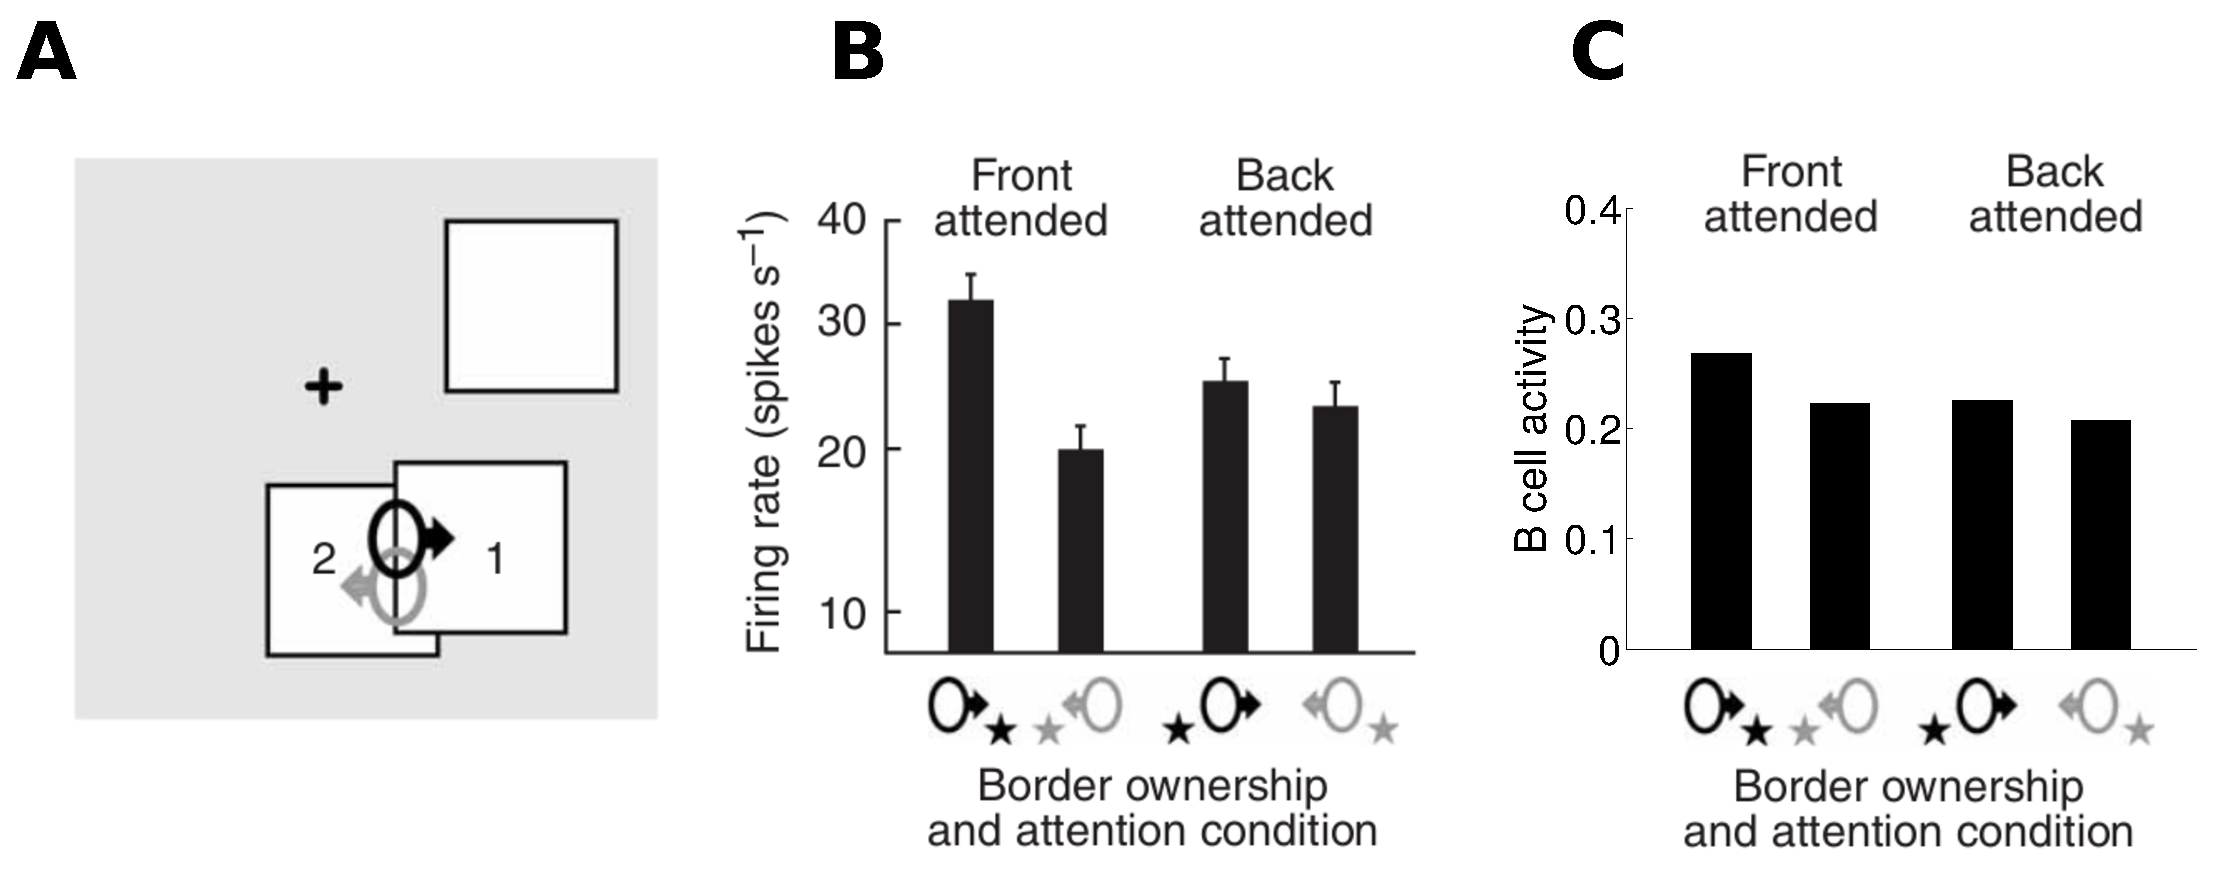
\includegraphics[width=0.75\textwidth]{Contour/figs/Fig7.eps}
\makeatletter
\let\@currsize\normalsize
\caption[Figure-ground segregation in the presence of noise]{Figure-ground segregation of a square object with aligned contour elements (top row) and with noise contour elements (top row). Shown are (left to right) the input stimulus, the edge cell activity (E), the border ownership assignment along edges (shown as the vector modulation index  $\overrightarrow{\mathbf{v}}$, section~\ref{sec:vmi}), the object grouping  neuron activity $(G_o)$ and the contour grouping activity $(G_c)$. Activities are normalized within each map, and warmer colors indicate higher activity (see color bar at right).}
\label{Fig:Square_Noise}
\end{figure}

We then extend this approach by adding additional oriented bars to the
stimulus, see Figure~\ref{Fig:Square_Noise}. In the top row of the figure, results are shown when the bar orientation within the figure differs from that of the background, similar to the texture-defined figures used in the \citet{Lamme95} experiments. In the bottom row, bars within and outside the figure are all oriented randomly, similar to the noise stimuli used in the \citet{Chen_etal14} study.  As in
Figure~\ref{Fig:BOS_timecourse}, we again show the responses of
different populations of neurons in our model.  For both types of
stimuli, the edges of the square, even when broken up into different
bars, are still enhanced while the background bars are suppressed,
especially within the square.  Interestingly, for the aligned stimulus
(top row), only the top and bottom edges of the square show border
ownership modulation. This may be an artifact of our modeling
procedure, where the edges of our figure are defined by contour elements instead of texture discontinuities. For the noise stimuli (bottom row), border ownership is still assigned correctly along the edge of the square, but the noise results in occasional nonzero border-ownership cell activity at other points in the image as well.  For both types of stimuli, grouping cell activity is still centered on the square, and contour grouping neurons still highlight the edges of the squares, but there is also noticeably increased noise.

\begin{figure}[t!]
\centering
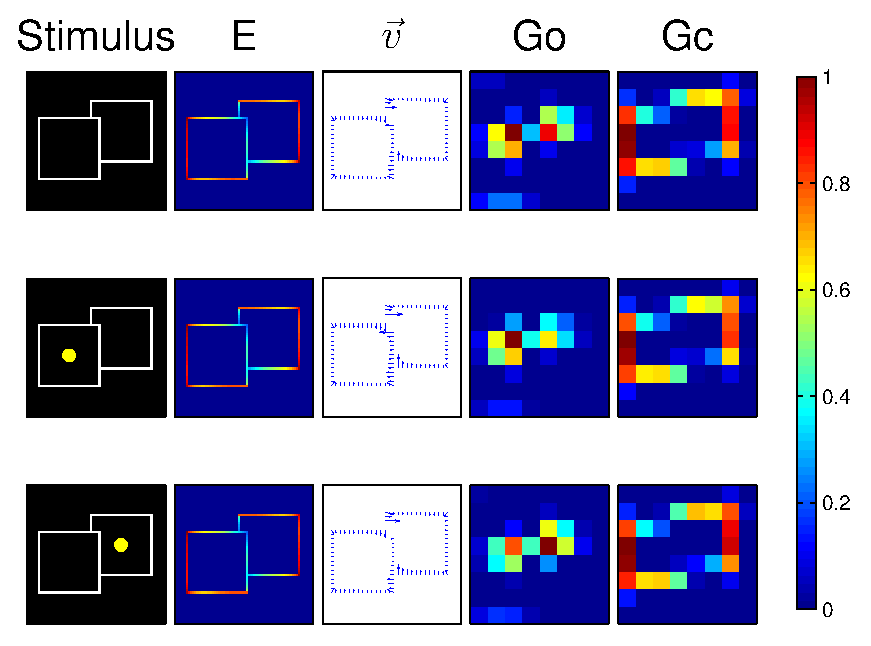
\includegraphics[width=\textwidth]{Contour/figs/Fig8.eps}
\makeatletter
\let\@currsize\normalsize
\caption[Quantitative comparison of attentional modulation across neuronal populations for figure in noise]{Attentional modulation of different neuronal populations aids figure-ground segregation in the presence of noise. Each panel (A-D) shows the means and standard deviations of neural activity with and without added attention over 100 different simulations. (A) Edge cell activity along the contour of the object shows enhancement with attention. (B) Edge cell activity in the center of the figure shows suppression with attention. (C) The BOS signal along the contour of the object shows enhancement with attention. (D) Object grouping cell (Go) activity centered on the object shows enhancement with attention.}
\label{Fig:Attention_modulation}
\end{figure}

\subsection{Interaction between border-ownership assignment and attention} 
\label{sec:BOS-att}

Although border ownership selectivity emerges independently of attention~\citep{Qiu_etal07}, attention may help to facilitate figure-ground segregation in the presence of noise.  For the square figure with noise, we found that in our model, attention increases the responses of neurons along the edge of the figure (unpaired t-test, $p=\num{2.32e-59}$) and suppresses those in the center (unpaired t-test,
$p=\num{3.42e-8}$). In addition, attention increases border-ownership
modulation along the edge of the figure (unpaired t-test, $p=\num{1.37e-143}$) and increases the activity of object grouping
neurons in the center of the figure (unpaired t-test, $p=\num{1.53e-239}$). All effects were small but highly significant,
and were based on the differences in summed activity of neurons along
the edge or center of the figure over a total of 100 simulations.
Figure~\ref{Fig:Attention_modulation} shows the average neural activity in the different populations of neurons in our model, with and without the effect of attention.  

Attention must also operate in cluttered environments where multiple
objects may be present. \cite{Qiu_etal07} studied border-ownership
responses in area V2 when two overlapping squares were presented and
attention was directed either to the foreground or background square. \cite{Mihalas_etal11b}, using a model closely related to ours but without $G_c$ cells, reproduced the experimental finding that border-ownership modulation was strong when attention was on the foreground figure but weak when attention was on the background
figure. Our model reproduces this finding, see Supplementary Figure
\ref{Fig:Overlap_Square}. The quantitative effect on border-ownership
selectivity is shown in Figure~\ref{Fig:Overlap_Square_exp_model}. 
Our model also reproduces the experimental finding that border-ownership modulation is strong when attention is on the foreground figure (Figure~\ref{Fig:Overlap_Square_exp_model}C,
``Front attended") and weak when attention is on the background
figure (Figure~\ref{Fig:Overlap_Square_exp_model}C, ``Back attended").

\begin{figure}[t!]
\centering
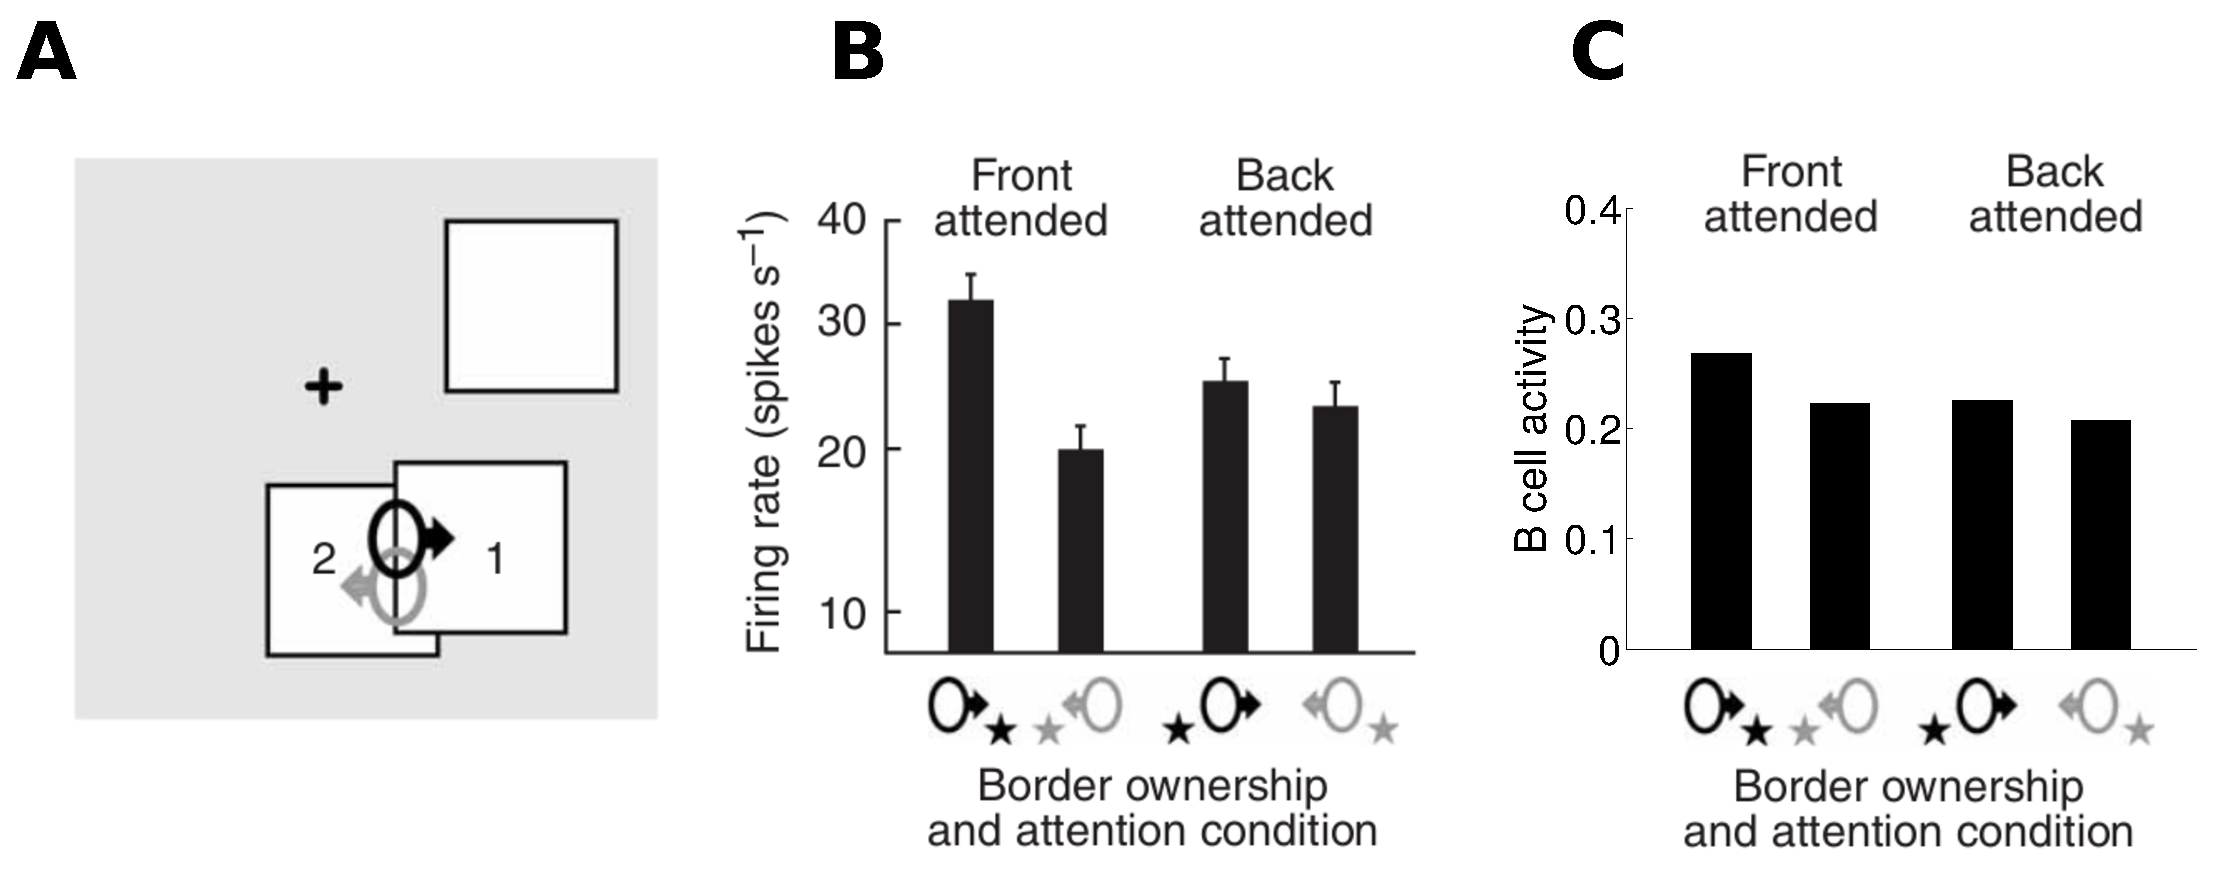
\includegraphics[width=0.75\textwidth]{Contour/figs/Fig9.eps}
\makeatletter
\let\@currsize\normalsize
\caption[Attention modulates border-ownership responses in the presence of multiple objects]{Quantitative comparison of model performance to  neurophysiological findings \citep{Qiu_etal07} for border-ownership coding of overlapping figures. (A) The stimulus configurations used are shown, with neurons coding right border ownership (black) and left border ownership (gray) when attention was focused on either foreground square 1 (front attended) or on background square 2 (back attended). (B) The responses of border-ownership selective cells recorded in V2 are shown:  bars indicate the average firing rate for each stimulus condition. (C) Model B cell responses to analogous stimulus conditions. For both the model and the experiments, border-ownership modulation was strong when attention was on foreground but weak when attention was on background. Panels~A and~B are modified from Figure~3 of~\cite{Qiu_etal07}.}
\label{Fig:Overlap_Square_exp_model}
\end{figure}

These results demonstrate that the object and contour grouping neurons
are able to assist with early level segmentation of objects in noise
and clutter.  Previous experimental studies have only tested squares
without noise, although the effect of figures defined by broken contours has been investigated before~\citep{Zhang_vonderHeydt10}.
Our results predict that border ownership assignment and grouping are
robust even in the presence of noise,  clutter, and interruptions in figure borders, and that attention may further aid this process.

\section{Discussion}
\label{sec:discussion}

\comment{In this study, we use computational models to elucidate the role of
attention and feedback in contour and object processing. Different
from many models that are tailor-made to reproduce one set of experimental
results, we demanded that our model explain data
from two different sets of experimental approaches, (1)~contour
integration and (2)~figure-ground segregation.  We hypothesize that
these two processes are fundamentally linked in terms of the larger
goal of image understanding.  Using the same set of model parameters,
we reproduced several experimental findings and generated non-trivial
predictions.}  

\subsection{Model predictions}

Our model predicts that attentional modulation is specific to the
attended contour or object, rather than being defined purely spatially. This is possible because, in our model, attention modifies firing rates of grouping cells, rather than of elementary feature-coding cells. Attending to the contour increases contour-response $d'$ in both V1 and V4, consistent with experimental results showing increased contour-related responses after animals had been trained to perform a contour detection task, compared to when they performed a separate set of tasks in which the contour was behaviorally irrelevant~\citep{Li_etal08a}. We note that \cite{Li_etal08a} only studied neural responses in V1, while our model makes predictions about attention-related changes to contour-response $d'$ in both V1 and V4.  We also find that attention modulates border ownership activity in V2 in an object-based manner. As a result, our model makes predictions about neural activity in visual areas V1, V2, and V4 across different stimuli and tasks.

We predict that the interaction of modulatory feedback from grouping
cells with local inhibition enhances the representation of the figure
and suppresses the representation of the background.  Indeed, our
model produces background suppression for isolated contours as well as
for figures embedded in noise.  We note that this prediction is
different from what others have observed in texture-defined figures
\citep{Lamme95,Lee_etal98a}, where there is generally response
enhancement of the center of the figure.  This difference may be due
to how the figure is defined, by its contour in our experiment and by
texture in \cite{Lamme95} and \cite{Lee_etal98a}. It is possible that if feedback from object grouping neurons is to the center of the
figure instead of its edges, we may observe enhancement of activity at
the center of the figure. Understanding how border-ownership assignment interacts with filling-in of surfaces is a future direction of research.  Furthermore we predict that attention, in addition to
enhancing the figure in an object-based manner, also helps to suppress
noise in the background.

We also predict that removing feedback from V4 to lower visual areas
reduces neural responses in V1, while having a smaller effect in V4.
The activity of V4 neurons is also affected due to the recurrency of
the network model. This could be tested experimentally by the same contour detection task used by~\cite{Chen_etal14}, and measuring the
contour-response $d'$ in V1 and V4 from reversible inactivation of
feedback connections. Although complete and selective deactivation of
V4 feedback to areas V1 and/or V2 is technically challenging, there
have been attempts to study the effect of this type of feedback either
through extra-striate lesions~\citep{Super_Lamme07} or reversible
inactivation~\citep{Jansen-Amorim_etal12}.  Anesthesia presumably also
decreases top-down influences, and indeed reduces contour-related V1
responses \citep{Li_etal08a} and figure-ground segregation
\citep{Lamme_etal98}.

\subsection{Comparison to other models}

Many have argued that contour integration and figure-ground segregation are largely local phenomena that rely on lateral connections \citep{Grossberg94, Grossberg97, Li98, Zhaoping05,  Piech_etal13}.  While some of these models include a role for top-down influences \citep{Li98,Piech_etal13}, they do not offer a specific mechanism by which higher visual areas representing object-level information selectively feed back to lower visual areas containing feature-level information about the object.  In contrast, our model is explicit in that feedback connections from higher visual areas modulate the responses of early feature-selective neurons involved in the related processes of contour integration and figure-ground segregation. Our model thus is a member of a broad class of theoretical models that achieve image understanding through bottom-up and top-down recurrent
processing~\citep{Ullman84,Hochstein_Ahissar02,Roelfsema_06,Epshtein_etal08}. In comparison to similar models, our model is able to reproduce
experimental findings from two traditionally separate fields of
study-- contour integration and figure-ground assignment. Importantly,
using the same set of network parameters, the grouping cells in our
model are able to represent proto-objects (both contours and extended
objects) and provide a perceptual organization of the scene. We 
show that this perceptual organization is critical for interfacing with top-down attention, and that it provides a general theoretical framework for understanding how feedback connections and an hierarchy of visual areas can be used to group together the features of an object. 

\subsection{Roles of V1 and V4 in visual processing}

While V1 neurons have small RFs that accurately code for orientation, V1 also shows strong background inhibition off the contour. This property allows V1 neurons to enhance contours and suppress noise in the image at a high spatial resolution. V4 neurons, on the other hand, have large RFs that integrate local feature information over large areas of visual space and provide a coarse, proto-object representation of contours and objects. Feedback from V4 can then be refined by the lateral connections present within early visual areas, which aids in the enhancement of the figure and its edges in the image.

Even when V1 neurons receive no feedback from V4, there is an increase in contour-response $d'$ with contour length (Figure~\ref{Fig:FB_att}). This contour facilitation is solely due to the excitatory lateral connections present in V1, and is weaker without feedback. As a result, feedback from V4 may not be necessary for contour facilitation, but it interacts with local lateral connections in a push-pull manner -- neurons along the contour are enhanced, while elements on the background are suppressed. Not surprisingly, removing this type of feedback has a larger effect on V1 neurons compared to V4 neurons, although the activity of V4 neurons is also affected due to the recurrency of the network model.

\subsection{Contour and object grouping neurons}

Contour grouping neurons have direct experimental support through the
recent neurophysiological experiments published by \cite{Chen_etal14}.
In our model, relatively few numbers of grouping neurons (both contour
and object) are required. The spatial resolution of the grouping
process does not need to be very high, as grouping cells only provide
a coarse template of the contours and objects present in the scene. Assuming that the activity of grouping cells represents proto-objects with a similar resolution as attention, the total number of grouping cells may be less than 2\% of the number of border-ownership cells~\citep{Craft_etal07}. In the contour integration experiments~\citep{Chen_etal14}, many V4 neurons were found to respond to straight, elongated contours, while in our model, only a subset of the grouping neurons are selective for contours. One possible explanation for this is overtraining -- monkeys performed the task a very large number of times each day for many months, and neural plasticity may have generated many V4 neurons which respond to contours. 

There is no unambiguous neurophysiological evidence for object grouping
neurons yet, although previous studies have found neurons in V4 that
respond to contour segments of various curvatures~\citep{Pasupathy_Connor02,Brincat_Connor04}. The receptive
fields of these neurons are similar to those proposed by \cite{Craft_etal07}. Other types of grouping neurons may also exist,
including those that respond to gratings~\citep{Hegde_vanEssen07},
illusory surfaces~\citep{Cox_etal13}, or 3D surfaces~\citep{He_Nakayama95,Hu_etal15a}. We do not attempt to model
the whole array of grouping neurons that may exist, but only those
necessary for reproducing the neurophysiological experiments referred
to here.

In our model, orientation-independent attentional input to contour
grouping cells was used to enhance neural responses to a contour at a
given location.  We note that this form of attention is analogous to
the size- and location tolerant attentional selection process proposed
by~\cite{Mihalas_etal11b}. The local circuitry of their model was able
to sharpen a relatively broad and nonspecific attentional input to
match the size and location of a figure in the visual
scene. Similarly, the local circuitry of our model transforms the
orientation-independent attentional input such that it only enhances
the contour of the correct orientation. We note that attention also has a suppressive effect in our model, essentially inhibiting unattended objects and locations. There is physiological support for this mechanism~\citep{Wegener_etal04,Hopf_etal06,Sundberg_etal09,Tsotsos11}. Furthermore, previous results show suppression of border-ownership activity along the shared edge of overlapping squares when the back square was attended, but not the front square~\citep{Qiu_etal07}. Finally, psychophysical experiments demonstrate an ``object superiority effect,'' where reaction times are fastest when attention is directed to targets that are part of the cued object, and slowest when targets are outside of an object~\citep{Egly_etal94,Kimchi_etal07}. 

Complementarily, feature-based attention acts broadly across the visual scene and increases the responses of all components that share similar feature attributes (\eg color, orientation, or direction of movement) with the attended component \citep{Motter94a,Treue_Trujillo99}. Orientation-specific forms of attention can enhance neural responses in V1 and V4, but do not significantly alter tuning curves or selectivity~\citep{McAdams_Maunsell99a}. Our model may be able to reproduce similar results by essentially changing the form of the attentional input to be orientation-specific, \ie top-down attention targets a \emph{single} population of contour grouping neurons with the same orientation preference. We expect that both object-based and feature-based forms of attention exist and can be flexibly used for different tasks.

\section{Conclusion}

Our model seeks to reproduce three different sets of experimental results, while making testable predictions for future experiments. 
We only included one scale of grouping neurons for simplicity, although 
multiple scales of grouping neurons are needed to account for the diversity in the scale of objects in the real world. Our model also assigns distinct roles to the different visual areas,  edge processing in V1, border ownership assignment in V2, and grouping of contours and objects in V4. However, the physiological properties of neurons in early visual areas have not been fully characterized, and neurons in these different areas may have additional ranges of selectivity than the ones we assign them in our model. Finally, our model operates on artificial images composed of simple shapes such as contours or square
figures. In order to truly understand grouping mechanisms in natural
vision, our model must also be able to operate on natural images as input, where the number of potential objects and features are much
richer. We propose such a model in the next chapter.

%%% Local Variables:
%%% mode: latex
%%% TeX-master: "../root"
%%% End:

\chapter{A recurrent neural network for figure-ground organization of natural scenes}
\label{sec:natural_image}
\chaptermark{Figure-ground organization of natural scenes}

\section{Introduction}

Figure-ground organization is critical for visual understanding of the world around us. The process typically involves some form of segmentation, or dividing the input image into regions corresponding to objects and background. The border between any two regions is usually ``owned" by a single object, and the correct assignment of each border to its corresponding object is thought to be a precursor to scene understanding. However, this task is difficult due to the clutter, occlusion, and wide variety of features present in natural scenes. This problem has long fascinated researchers, including those from the fields of psychology~\citep{Wertheimer23,Koffka35}, neuroscience~\citep{Zhou_etal00,Craft_etal07}, and computer vision~\citep{Sajda_Finkel95,Ren_etal06,Teo_etal15,Wang_Yuille16}.
Despite this long line of research, our understanding of the neural basis of figure-ground organization remains surprisingly limited.

A key insight from neuroscience was the discovery of border-ownership
cells. Border-ownership selectivity is a property of a majority of the
neurons in V2, which encodes where an object is located relative to the
neuron's receptive field~\citep{Zhou_etal00}. When the edge of an object is presented in its receptive field (RF), a border-ownership cell will respond with different firing rates depending on where the object is located. For the example cell shown in Figure~\ref{Fig:experiments}A, objects placed to the upper right of the cell's RF (stimuli outlined in red) cause the cell to fire at a higher firing rate compared to objects placed to the lower left of the cell's RF (stimuli outlined in blue). Importantly, the local stimulus within the cell's RF is identical in both cases. Border-ownership coding has been studied using a wide variety of artificial stimuli, including those defined by luminance~\citep{Zhou_etal00}, motion~\citep{vonderHeydt_etal03a}, disparity~\citep{Qiu_vonderHeydt05}, and transparency~\citep{Qiu_vonderHeydt07}, and more recently, natural stimuli such as faces~\citep{Hesse_Tsao16,Ko_vonderHeydt17} and complex natural scenes~\citep{Williford_vonderHeydt16}.

To explain this phenomenon, some computational models assume that
border-ownership coding is achieved purely by feedforward mechanisms, such as the asymmetric organization of surrounds \citep{Nishimura_Sakai04,Nishimura_Sakai05,Sakai_etal12} or global surround inhibition~\citep{Super_etal10}. Pure feedforward models predict similar latencies of the border-ownership signal regardless of the stimulus, but recent results show that border-ownership assignment of stimuli with illusory contours is delayed by $\sim30$ms compared to full stimuli~\citep{Hesse_Tsao16}. Other models propose  propagation of neural activity along horizontal connections within early visual
areas using a diffusion-like process \citep{Grossberg94,Sajda_Finkel95,
Baek_Sajda05, Kikuchi_Akashi01, Pao_etal99,Zhaoping05,Zucker12}. However, these models have difficulties explaining the fast establishment of border ownership which appears about 25ms after
the first stimulus response \citep{Zhou_etal00}.  Propagation along horizontal fibers over the distances used in the experiments would imply a delay of at least $\sim70$ms \citep[][based on the conduction velocity of horizontal fibers in primate V1 cortex; we are not aware of corresponding data for V2]{Girard_etal01}. Furthermore, such models are difficult to reconcile with the observation that the time course of border-ownership coding is largely independent of figure
size~\citep{Sugihara_etal11}.

An alternative computational model involves populations of grouping
($\mathcal{G}$) cells which explicitly represent (in their firing rates) the perceptual organization of the visual scene~\citep{Craft_etal07,Mihalas_etal11b}. These cells are reciprocally connected to border-ownership selective ($\mathcal{B}$) cells through feedforward and feedback connections. The combined activation of grouping cells and cells signaling local features represents the presence of a ``proto-object''~\citep[we borrow this term from the perception literature;][]{Rensink00a}, resulting in a structured perceptual organization of the scene. This proto-object based approach is consistent with psychophysical and neurophysiological studies
\citep[\eg][]{Duncan84,Egly_etal94,Scholl01,Kimchi_etal07,Qiu_etal07,Ho_Yeh09,Poort_etal12}. A feedforward version of this model has been applied to natural scenes, where it outperformed other models in predicting the locations of human eye fixations~\citep{Russell_etal14}.

\begin{figure}[t!]
\centering
\includegraphics[width=\textwidth]{NaturalImage/figs/exp_data.eps}
\makeatletter
\let\@currsize\normalsize
% simplify caption
\caption[Consistency of border-ownership coding across square and natural scene stimuli]{Consistency of border-ownership coding. (A) Border-ownership coding for an example cell. The cell has a preference for objects located to the upper right of its receptive field (RF) on both the square and natural scene stimuli, as indicated by higher firing rates. Red circles indicate the size and location of the cell's RF. Stimuli with objects to the upper right of the cell's RF (``preferred" side) are outlined in red, while stimuli with objects to the lower left of the cell's RF (``non-preferred" side) are outlined in blue. The cell's postimulus time histogram (PSTH) for the preferred side is shown by the red trace, while the PSTH for the non-preferred side is shown by the blue trace. Shading indicates 95\% confidence intervals.}
\label{Fig:experiments}
\end{figure}

A substantial fraction of neurons show consistent border-ownership coding across natural scenes that matches their preference on artificial stimuli, with the timing of border-ownership signals being similar for both types of stimuli (Figure~\ref{Fig:experiments}B). However, with the exception of a single computational model~\citep{Sakai_etal12}, we are not aware of any models that have quantitatively tested border-ownership selectivity on natural scenes. Here, we propose a model based on recurrent connections that is able to explain border-ownership coding in natural scenes. We compare our model results with experimental results, and find a good match both in the timing of the border-ownership signals as well as the consistency of border-ownership coding across scenes. In order to compare our model with other computer vision approaches, we also benchmarked our model on a standard contour detection and figure-ground assignment dataset~\citep{Martin_etal01} and achieve performance comparable to these other approaches.

\begin{figure}[t!]
\centering
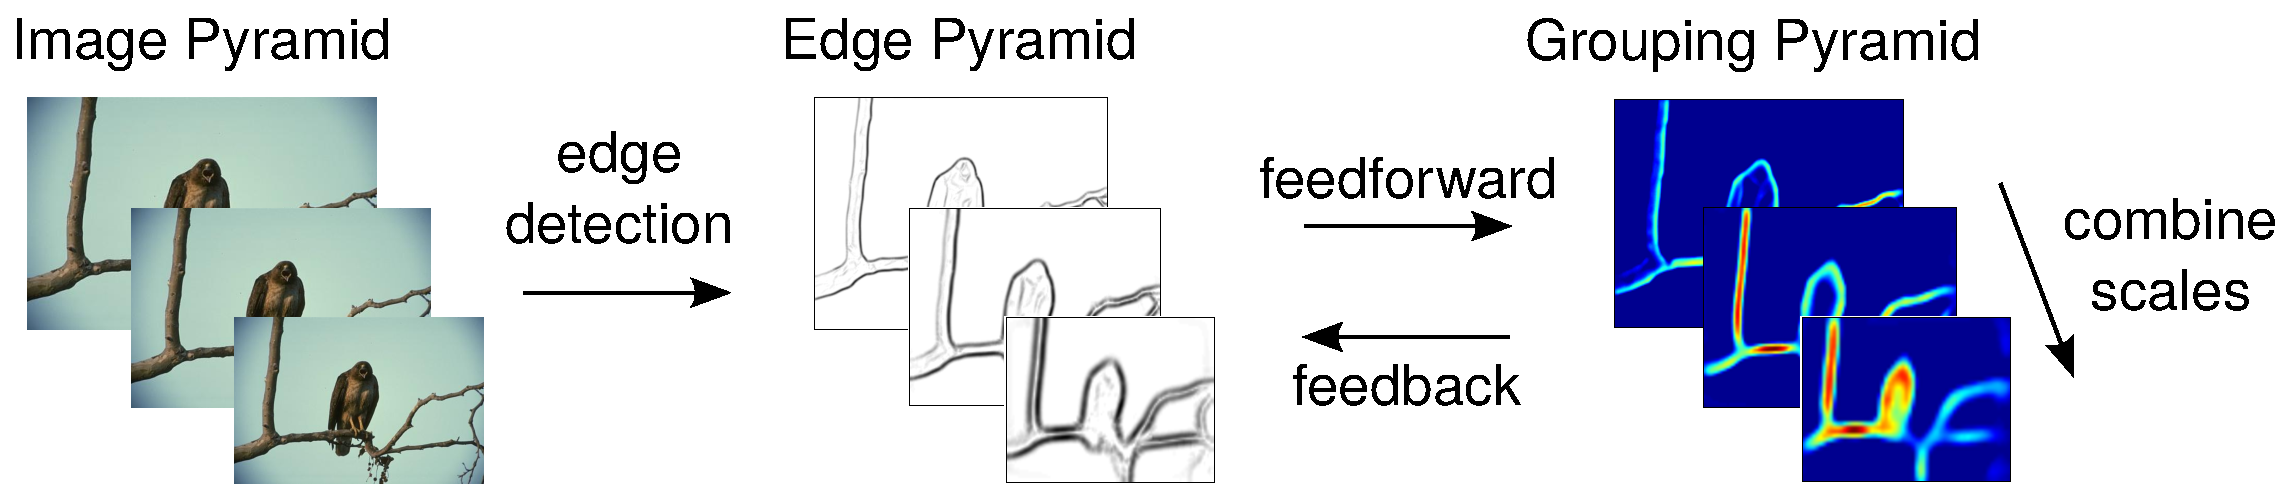
\includegraphics[width=\textwidth]{NaturalImage/figs/model_scheme_new.eps}
\makeatletter
\let\@currsize\normalsize
% simplify caption
\caption[Overview of the model for figure-ground organization of natural scenes]{Overview of the model. The image is first successively downsampled in half-octaves to create an image pyramid (only three scales are shown). The same set of feedforward and feedback grouping operations is then applied at each level of the pyramid to achieve scale invariance. Feedback from grouping cells is combined across scales so that global context information can influence figure-ground segmentation. The model is run for a total of 10 iterations (one iteration includes a feedforward and a feedback pass through the model), and our final results are based on neural activity from the highest resolution scale of the image pyramid.}
\label{Fig:model_overview}
\end{figure}

\section{Methods} 
\label{sec:model}
\subsection{Model Structure}

Our approach is an extension of the proto-object based model of saliency proposed by~\cite{Russell_etal14} and includes recurrent connections for figure-ground assignment. At the core of our model is a grouping mechanism which estimates figure-ground assignment within the input image using proto-objects of varying spatial scales and feature types. These proto-objects provide a coarse segmentation of the image through perceptual organization of the scene into regions corresponding to objects and background.
 
To achieve scale invariance, the algorithm successively downsamples the input image in steps of $\sqrt2$ to form an image pyramid spanning five octaves (Figure~\ref{Fig:model_overview}). The $k$th level of the pyramid is denoted using the superscript $k$. Unless explicitly stated, any operation applied to the pyramid is applied independently to each level and each feature type. Each layer of the network represents neural activity, which can either be propagated from one layer to another via feedforward or feedback connections since our model is recurrent. We use a filter-based approach, where the receptive fields of neurons are described by kernels and the correlation operation is used to calculate the neural response to an input. The model was implemented using MATLAB (Mathworks, Natick, MA,
USA).

The first stage of the model extracts edges from the input image based on either luminance or color information (Figure~\ref{Fig:model_overview}). We use the combination of receptive fields (CORF) operator, which is a model of V1 simple cells with push-pull inhibition~\citep{Azzopardi_etal14}. We chose the CORF operator due to its texture suppression properties, which can be beneficial when applied to natural images. Our model does not require a specific edge detection method and could be modified to use other front-end edge detectors (\eg Gabor filters). In the following, we only describe model computations on the luminance channel, but the exact same computations are also performed on the two color channels (\ie red-green and blue-yellow). As in~\citet{Russell_etal14}, the color channels were computed according to the methods outlined in the original~\citet{Itti_etal98a} visual saliency model.

For a given scale $k$, the output of the edge detection stage of the model are simple ($\mathcal{S}$) cells of eight different orientations $\theta$ and two contrast polarities, termed $\mathcal{S}^k_{\theta,L}(x,y)$ and $\mathcal{S}^k_{\theta,D}(x,y)$ (\ie for light-dark edges $L$ and dark-light edges $D$). For the two color channels, the edge polarities are determined by color-opponent responses (\eg red-green edges and green-red edges). Only the signal strength at the optimal orientation at each spatial location was used as input to the network. This simplification significantly reduces computation time by eliminating the calculation of responses for the non-optimum orientations.

In contrast to previous approaches which combine simple cell responses into a contrast-invariant complex cell response~\citep{Russell_etal14}, we keep the contrast-sensitive
$\mathcal{S}$ cell responses as they provide an informative cue for grouping along object edges. Objects tend to maintain similar contrast polarity along their boundaries, which may be useful for accurately determining figure-ground relationships. As a result, we have two sets of responses at each layer of our network corresponding to the two different types of contrast polarity.

Next, for a given angle~$\theta$, each $\mathcal{S}$ cell feeds into an opposing pair of border-ownership ($\mathcal{B}$) cells. As a result, $\mathcal{B}$ cells are also sensitive to contrast polarity, which is consistent with experimental findings~\citep{Zhou_etal00}.
For each contrast polarity, we used one-to-one connections between $\mathcal{S}$ cells of one orientation and the corresponding pair of
$\mathcal{B}$ cells with the same preferred orientation, but opposing side-of-figure preferences.
\begin{equation}
\begin{split}
\mathcal{B}^k_{\theta,L} = \mathcal{S}^k_{\theta,L}(x,y)\\
\mathcal{B}^k_{\theta+\pi,L} = \mathcal{S}^k_{\theta,L}(x,y)\\
\end{split}
\end{equation}
\begin{equation}
\begin{split}
\mathcal{B}^k_{\theta,D} = \mathcal{S}^k_{\theta,D}(x,y)\\
\mathcal{B}^k_{\theta+\pi,D} = \mathcal{S}^k_{\theta,D}(x,y)
\end{split}
\end{equation}

To infer whether the edges in $\mathcal{B}^k_{\theta,L}(x,y)$ and $\mathcal{B}^k_{\theta,D}(x,y)$ belong to figure or ground, knowledge of proto-objects in the scene is required. This context information is retrieved from a grouping mechanism (Figure~\ref{Fig:model_overview}). Grouping cells ($\mathcal{G}$) integrate information from $\mathcal{B}$
cells, and either respond to light objects on dark backgrounds, $\mathcal{G}^k_{L}(x,y)$, or dark objects on light backgrounds, $\mathcal{G}^k_{D}(x,y)$. This computation is similar to the use of center-surround cells in a feedforward version of the model~\citep{Russell_etal14}. In contrast to their approach, our model does not require an additional class of center-surround cells, but instead allows $\mathcal{G}$ cells to directly integrate local feature information from $\mathcal{B}$ cells and then bias the activity of these same cells using reciprocal feedback connections. Our model runs in an iterative manner, with one iteration corresponding to a feedforward and feedback pass through the model. $\mathcal{G}$ cell activity is combined across scales before each feedback pass, which allows the model to more accurately determine figure-ground assignment in a scale-invariant manner (Figure~\ref{Fig:model_overview}).

\begin{figure}[t!]
\centering

\includegraphics[width=\textwidth]{NaturalImage/figs/model_circuit.png}
\makeatletter
\let\@currsize\normalsize
% simplify caption
\caption[Structure of the recurrent neural network model for figure-ground organization of natural images]{Structure of the recurrent neural network. Each circle stands for a population of neurons with similar receptive fields and response properties. Red and blue lines represent excitatory and inhibitory projections, respectively. Solid and dashed lines represent purely feedforward and reciprocal feedforward/feedback connections, respectively. Edges and other local features of a figure (black square outline) activate simple cells ($\mathcal{S}$) whose receptive fields are shown by green ellipses. $\mathcal{S}$ cells project to border-ownership cells ($\mathcal{B}$) that have the same preferred orientation and retinotopic position as the $\mathcal{S}$ cells they receive input  from. However, for each location and preferred orientation there are  two $\mathcal{B}$ cell populations with opposite side-of-figure preferences, in the example shown $\mathcal{B}_{\pi}$ whose neurons respond preferentially when the foreground object is to the left of their receptive fields and $\mathcal{B}_{0}$ whose members prefer the foreground to the right side of their receptive fields. $\mathcal{B}$ cells have reciprocal, feedforward excitatory and feedback modulatory connections with grouping cells, $\mathcal{G}$, which integrate global context information about objects. The receptive field of a $\mathcal{G}$ cell is shown by the purple annulus. Opposing $\mathcal{B}$ cells compete indirectly {\em via} feedback inhibition  from $\mathcal{G}$ cells, which bias their activity and thus generate the border-ownership signal used to determine figure-ground assignment.}
\label{Fig:model}
\end{figure}

A more detailed view of the structure of our model is shown in Figure~\ref{Fig:model}. $\mathcal{G}$ cells integrate the $\mathcal{B}$ cell activity in an annular fashion. This allows $\mathcal{G}$ cells to show preference for objects whose borders exhibit the Gestalt principles of continuity and proximity. $\mathcal{G}$ cell activity is defined according to
\begin{equation}
\begin{split}
\mathcal{G}_{L}^k(x,y) = &\Bigg\lfloor\sum_\theta
                     [\mathcal{B}^k_{\theta,L}(x,y)-\mathcal{B}^k_{\theta+\pi,L}(x,y)]\ast v_\theta(x,y)\Bigg\rfloor
\end{split}
\label{eq:G_L}
\end{equation}
\begin{equation}
\begin{split}
\mathcal{G}_{D}^k(x,y) = &\Bigg\lfloor\sum_\theta
                     [\mathcal{B}^k_{\theta,D}(x,y)-\mathcal{B}^k_{\theta+\pi,D}(x,y)]\ast v_\theta(x,y)\Bigg\rfloor
\end{split}
\label{eq:G_D}
\end{equation}

where $\lfloor \cdot \rfloor$ is a half-wave rectification, and $\ast$ is the correlation operator defined as

\begin{equation}
f(x,y)\ast g(x,y) = \sum_{m=-\infty}^{\infty}\sum_{n=-\infty}^{\infty}f(m,n)g(x+m,y+n)
\end{equation}

$v_{\theta}$ is generated using the von Mises distribution as follows
\begin{equation}
v_\theta(x,y) = \frac{\exp\left[(\sqrt{x^2+y^2}-R_0)\cos(\tan^{-1}(\frac{y}{x})-\theta+\frac{\pi}{2})\right]}{2\pi I_0(\sqrt{x^2+y^2}-R_0)}
\label{eq:vonMises}
\end{equation}

where $R_0$ is the radius of the grouping cell receptive field, set to 2 pixels, and $\theta$ is the desired angle of the mask. The factor $\frac{\pi}{2}$ rotates the mask to ensure it is correctly aligned with the edge cells. $I_0$ is the modified Bessel function of the first kind. $v_\theta$ is then normalized according to
\begin{equation}
v_\theta(x,y) = \frac{v_\theta(x,y)}{\max(v_\theta(x,y))}
\end{equation}

On the first iteration, since there is no difference in activity between each pair of $\mathcal{B}$ cells as they receive the same initial bottom-up input, we omit the inhibition by the non-preferred
$\mathcal{B}$ cells and only use the activity of the preferred
$\mathcal{B}$ cells (eqs.~\ref{eq:G_L} and~\ref{eq:G_D}). On subsequent iterations, we include the inhibitory term. We also implement a simple form of local inhibition between the two grouping pyramids, $\mathcal{G}^k_{L}(x,y)$ and $\mathcal{G}^k_{D}(x,y)$. At each spatial location, only one type of $\mathcal{G}$ cell should be active, representing either a light or dark object at that location. For each level of the pyramid $k$, we perform a max operation as follows
\begin{equation}
	\mathcal{G}^k_{L}(x,y)=
	\begin{cases}
	\mathcal{G}^k_{L}(x,y) \:\;&if\;\mathcal{G}^k_{L}(x,y) > \mathcal{G}^k_{D}(x,y)\\
	0\;&otherwise
	\end{cases}\\
\end{equation}
\begin{equation}
	\mathcal{G}^k_{D}(x,y)=
	\begin{cases}
	\mathcal{G}^k_{D}(x,y) \:\;&if\;\mathcal{G}^k_{D}(x,y) > \mathcal{G}^k_{L}(x,y)\\
	0\;&otherwise
	\end{cases}\\
\end{equation}

Feedback from $\mathcal{G}$ cells to $\mathcal{B}$ cells is used to bias the responses of the $\mathcal{B}$ cells to correctly signal figure-ground assignment. The feedback depends on the contrast polarity of the $\mathcal{G}$ cell and the $\mathcal{B}$ cell.

$\mathcal{B}^k_{\theta,L}$, the border-ownership activity for a light object on a dark background is given by
\begin{equation}
\begin{split}
\mathcal{B}^k_{\theta,L}(x,y) = &2\mathcal{S}^k_{\theta,L}(x,y)\\
            &\times\frac{1}{1+\exp\Big(-(\sum_{j\geq k}\frac{1}{2^{j-k}} v_{\theta+\pi}(x,y) \ast \mathcal{G}^j_{L}(x,y)-\sum_{j\geq k}\frac{1}{2^{j-k}} v_{\theta}(x,y) \ast \mathcal{G}^j_{D}(x,y))\Big)}
\end{split}
\label{eq:border-orientation1}
\end{equation}

$\mathcal{B}^k_{\theta,D}$, the border-ownership activity for a dark object on a light background is given by
\begin{equation}
\begin{split}
\mathcal{B}^k_{\theta,D}(x,y) = &2\mathcal{S}^k_{\theta,D}(x,y)\\
            &\times\frac{1}{1+\exp\Big(-(\sum_{j\geq k}\frac{1}{2^{j-k}} v_{\theta+\pi}(x,y) \ast \mathcal{G}^j_{D}(x,y)-\sum_{j\geq k}\frac{1}{2^{j-k}} v_{\theta}(x,y) \ast \mathcal{G}^j_{L}(x,y))\Big)}
\end{split}
\label{eq:border-orientation2}
\end{equation}

where $v_{\theta}$ is the kernel responsible for mapping object activity in the grouping pyramids back to the objects edges, and the term $2^{-j}$ normalizes the $v_{\theta}$ operator across scales. The logistic function in the equations above enforces a form of competition between $\mathcal{B}$ cells such that their total activity is always conserved, and each $\mathcal{B}$ cell has activity between the range of zero and two times their initial bottom-up input activity, $\mathcal{S}^k_{\theta}(x,y)$.

In the equations above, feedback from $\mathcal{G}$ cells to $\mathcal{B}$ cells is contrast-sensitive. $\mathcal{B}$ cells receive excitatory feedback from $\mathcal{G}$ cells of the same contrast polarity on their preferred side and inhibitory feedback from $\mathcal{G}$ cells of the opposite contrast polarity on their non-preferred side. This is motivated by neurophysiological results which show that image fragments placed within the extra-classical receptive field of a border-ownership neuron can cause enhancement of the neuron's activity when placed on its preferred side, and suppression if placed on the non-preferred side \citep{Zhang_vonderHeydt10}. Furthermore, modulating the bottom-up $\mathcal{S}$ cell responses with $\mathcal{G}$ cell activity summed across spatial scales ensures that the $\mathcal{B}$ cell responses are scale-invariant. Neurophysiological results show border-ownership coding for stimuli of varying sizes, with the latency of the border-ownership signal being relatively independent of the size of the figure~\citep{Zhou_etal00,Sugihara_etal11}.

Figure-ground assignment should be robust for both light objects on dark backgrounds and dark objects on light backgrounds. In our model, this is achieved by computing $\mathcal{B}$ cell activity independently for each contrast polarity and then summing this activity to give a final border-ownership response independent of figure-ground contrast polarity. The $\mathcal{B}$ cell responses for light and dark objects are combined to give a contrast polarity invariant response
\begin{equation}
\mathcal{B}^k_{\theta}(x,y) =
\mathcal{B}^k_{\theta,L}(x,y)+\mathcal{B}^k_{\theta,D}(x,y)
\label{eq:BOS}
\end{equation}

The sign of the difference $\mathcal{B}_{\theta}(x,y)-\mathcal{B}_{\theta+\pi}(x,y)$ determines the direction of border ownership at pixel $(x,y)$ and orientation $\theta$. Its magnitude gives a confidence measure for the strength of border ownership.

Similarly, the $\mathcal{G}$ cell responses for light and dark objects are combined to give a contrast polarity invariant response
\begin{equation}
\mathcal{G}^k(x,y) =
\mathcal{G}^k_{L}(x,y)+\mathcal{G}^k_{D}(x,y)
\label{eq:G}
\end{equation}

The $\mathcal{G}$ pyramid from eq.~\ref{eq:G_L} and eq.~\ref{eq:G_D}, summed across both the light and dark channels, along with the figure-ground assignments in the $\mathcal{B}$ cells, is the output of the grouping algorithm and provides a perceptual organization of the visual scene.

As mentioned previously, we use both luminance and color information from the image in order to perform the grouping operation. The same exact operations that were performed on the luminance channel are also performed on the two color channels. We combine the final outputs of the $\mathcal{B}$ and $\mathcal{G}$ cells with an 80\% weighting for the luminance channel and a 10\% weighting for both the red-green and blue-yellow color channels. This choice of weighting does not qualitatively change our results.

\subsection{Model Implementation}
\label{sec:implementation}

All simulations were performed on a 300-core CPU cluster running Rocks 6.2 (Sidewinder), a Linux distribution intended for high-performance computing. This allowed us to independently run our model on different images, speeding up our testing time. We ran the model for a total of 10 iterations, with each iteration being one feedforward pass of $\mathcal{B}$ cell to $\mathcal{G}$ cell activity, followed by one feedback pass of $\mathcal{G}$ cell to $\mathcal{B}$ cell activity (Figure~\ref{Fig:model_overview}). We generally found that the model converged after a few iterations. The final $\mathcal{G}$ cell activity was summed across scales. Contour detection and figure-ground assignment results are computed from the population of $\mathcal{B}$ cells at the highest resolution level of the image pyramid, which had the same resolution as the input image. $\mathcal{B}$ cell activity is converted into a population vector code by summing the final activity across orientations, where the magnitude of the resulting vector represents the border-ownership signal (or edge strength), and the direction of the vector provides a continuous figure-ground orientation label. For a given image, we normalize the border ownership signal at each pixel $(x,y)$ by the maximum border ownership signal across the entire image, such that the border ownership signal is bounded between -1 and +1.

We benchmarked our model on the publicly available Berkeley Segementation Dataset \citep{Martin_etal01}. We did this in the context of two tasks: contour detection and figure-ground assignment. Each dataset includes 100 to 200 test images, and we report F-scores (harmonic mean of precision and recall) for the contour detection task and mean accuracy (percent of correctly labeled figure-ground edges) for figure-ground assignment task averaged over all test images. We used publicly available benchmarking code to do our analysis and comparisons with other approaches.

\subsection{Model to Cell Comparison}
\label{sec:cell_model}
% Edit this section based on our final choice of analysis
To compare our model with experimental results, we used a publicly available dataset of border-ownership cell responses recorded during viewing of natural scenes~\citep{Jonathan_data}. More details about the stimuli, experimental design, and data analysis can be found in the corresponding paper~\citep{Williford_vonderHeydt16}.
% Edit this accordingly...
The dataset includes border-ownership signals (BOS) for each scene that was viewed by each recorded cell. In order to compare our model with the experimental results, we calculated the model's border ownership signal for the same set of scenes shown to the cells. We quantified model performance by using a combination of the cosine similarity metric, regression goodness of fit, and equivalence testing, which are explained in more detail below.
%
%We examined two aspects of the dataset. First, we looked at the model responses over a large numver of scenes as a means to estimate the model's consistency. Our results show the model's border ownership responses sorted across scenes.

\subsubsection{Cosine Similarity}
To compare the model with cells from the experiment, we first chose a subset of the cells ($N=13$) that had highly consistent border-ownership responses (defined as having the same side of border ownership on $>$80\% of their tested scenes). To compare the BOS response of a cell to another cell or to the model on the set of common scenes viewed by both, we used the cosine similarity metric, which is defined as

\begin{equation}
\cos(\theta) = \frac{A \cdot B}{||A||_{2}||B||_{2}} = \frac{\sum\limits_{i=1}^{n}A_{i}B_{i}}{\sqrt{\sum\limits_{i=1}^{n}A_{i}^2}\sqrt{\sum\limits_{i=1}^{n}B_{i}^2}}
\label{eq:cos_sim}
\end{equation}
where $A_i$ and $B_i$ are components of the vectors $A$ and $B$ respectively.

% define with equation?
The cosine similarity is bounded between -1 and +1, with the geometric interpretation that the metric measures the cosine of the angle between two vectors in a high dimensional space. Two vectors which are exactly the same will have a cosine similarity of 1, two vectors that are exactly opposite will have a cosine similarity of -1, and a cosine similarity of 0 indicates two vectors that are orthogonal or decorrelated. In our case, we can treat the responses of the model or a given cell on a set of scenes as a vector in a high-dimensional space (with each axis being the BOS for one scene) and we can then compute the cosine similarity between any two vectors (\eg between one cell and another cell or between the model and a cell). We also explored the use of other similarity metrics, such as the Pearson correlation coefficient ($r$), but found that these metrics often unfairly reduced the similarity measure due to mean centering of the BOS responses.

\subsubsection{Equivalence Testing}
To test the hypothesis that the model performs similarly to cells from the experiment, we use equivalence testing, which has more traditionally been used in the bioequivalence setting, for example, to compare whether the efficacy of a new drug is similar to that of an existing drug on the market. In standard hypothesis testing, the null hypothesis is that mean of the two distributions are not statistically different. However, failure to reject the null hypothesis is not sufficient evidence to conclude that the two distributions are similar, as the test may also fail due to not having enough statistical power. In equivalence testing, the null hypothesis is instead that the means of the two distributions differ by a pre-determined ``zone of scientific significance." The alternative hypothesis (where the burden of proof lies) is that the means of the two distributions are actually the same. In our case, the equivalence test is calculated by either using two one-sided $t$-tests or computing confidence intervals on the difference between the model-cell and cell-cell cosine similarity distributions, and determining whether this confidence interval lies within the pre-determined zone of scientific significance. We chose a zone between -0.2 - 0.2, which represents $\pm$10\% of the full range of possible cosine similarity values.

\subsubsection{Goodness of Fit}
In order to quantify model performance on a per-cell basis, we performed linear regression on the cell's border-ownership responses across scenes (ordinate) against the model's border-ownership responses across the same set of scenes (abscissa). For each regression calculation, we forced the least-squares regression line through the origin because the sign of the border-ownership signal for a given neuron is arbitrary. Two border-ownership selective neurons responding to the same edge can have opposite side-of-figure preferences, and which direction we assign a positive value is arbitrary. This ambiguity means that the line of best fit must be invariant against reflecting any data points about the origin, which is why the fitted line must pass through the origin.

However, each cell's response contains a repeatable component (in response to the same stimulus and which we attempt to capture with our model) and a noise component (which is completely random). Because our model is deterministic, it is unable to capture the noise component present in the responses of cells. The linear regression provides a measure of the variance that can be explained by our grouping model. However, we only care about the explainable variance, which is the total response variance minus the noise variance, which can be estimated from a small number of stimulus presentations from experiments. As a result, we defined a goodness of fit measure for the regression by computing the fraction of explainable variance that can actually be explained by the model. We follow the general methods put forth in~\citet{DiCarlo_etal98} for calculating the goodness of fit measure.

\begin{figure}[t!]
\centering
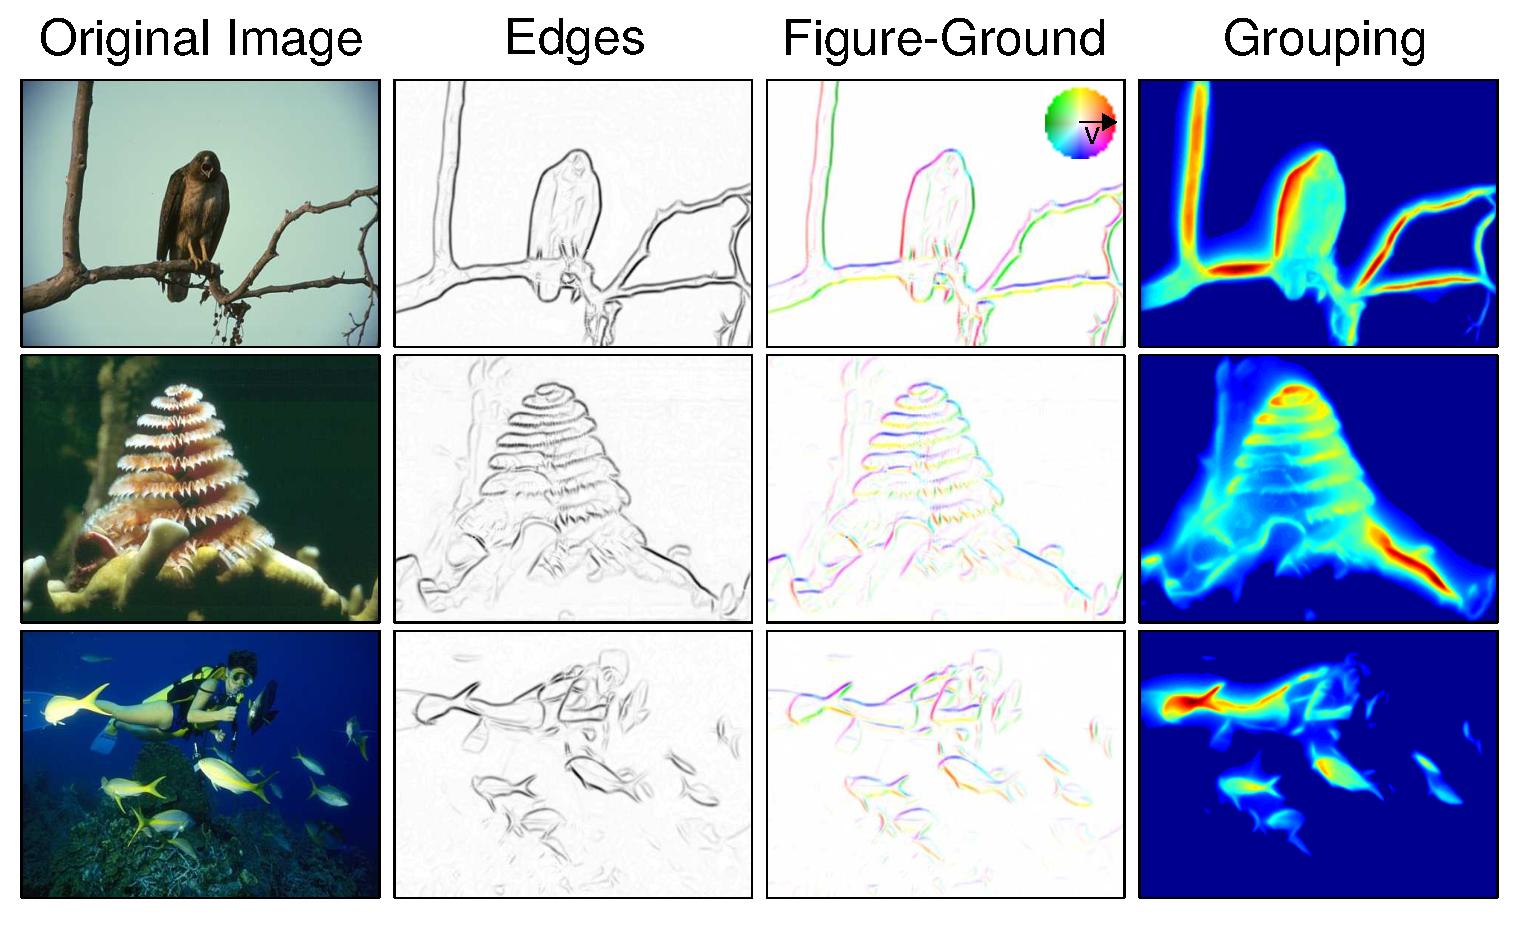
\includegraphics[width=\textwidth]{NaturalImage/figs/results_new}
\makeatletter
\let\@currsize\normalsize
% simplify caption
\caption[Model results on images from the BSDS dataset]{Results of our model on example images from the Berkeley Segmentation Dataset. Columns from left to right are the original images, the edge maps, the border-ownership cell activity (representing figure-ground assignment), and also grouping cell activity. For the figure-ground assignment, the color of each edge is represented by a hue and a saturation value (see color wheel insert). The hue of the edge represents the figure-ground orientation label with the arrow convention shown in the color wheel (\eg red represents an object pointing to the right) and the saturation of the edge represents the strength of the border-ownership signal.}
\label{Fig:results_summary}
\end{figure}


\section{Results}
\label{sec:results}

\subsection{Evaluation of the model on standard benchmarks}
% List which algorithms we compared against here
We benchmarked our model on the Berkeley Segmentation Dataset~\citep{Martin_etal01}. We did this for two separate tasks: 1) a contour detection task and 2) a figure-ground assignment task. Importantly, our model uses the same set of parameters for both tasks, and parameters were not tuned separately for each task. Examples of our model output are shown in Figure~\ref{Fig:results_summary}. Here, we show the original input image, the edge signals, the border-ownership signals, and the final grouping maps. We hypothesize that the border-ownership signal is a good correlate of the perceptual saliency of object contours. As a result, we use the border-ownership signal (independent of figure-ground orientation) as the output for the contour detection task. We quantify our results on the contour detection task using the F-score, which is the harmonic mean of accuracy and precision of contour detection. For the contour detection task, we compare our approach to three different approaches: ultrametric contour map~\citep[][gPb-owt-ucm]{Arbeleaz_etal11}, structured edges~\citep[][SE]{Dollar_Zitnick15}, and structured random forests~\citep[][SRF]{Teo_etal15}. Overall, we achieved an F-score of 0.64 on the contour-detection task. State-of-the-art computer vision models achieve F-scores on the order of 0.73 (all three approaches gave similar results). Our model does not perform as well as these other approaches, which may be the result of the limitations in the initial edge detection method we used in our model.

%% Insert table of results here for contour detection and figure-ground
\begin{table}[h!]
\centering
\begin{tabular}{|c|c|c|c| } 
 \cline{2-4}
 \multicolumn{1}{c}{} & \multicolumn{3}{|c|}{\textbf{BSDS500}} \\
 \cline{2-4}
 \multicolumn{1}{c|}{} & ODS & OIS & AP\\ 
 \hline
 Human & 0.80 & 0.80 & -\\ 
 \hline
  Our approach & 0.64 & 0.65 & 0.51 \\
 gPb-owt-ucm & 0.73 & \textbf{0.76} & 0.73 \\
 SE & 0.73 & 0.75 & \textbf{0.77} \\
 SRF & 0.73 & 0.74 & 0.76 \\
 \hline
\end{tabular}
\makeatletter
\let\@currsize\normalsize
\caption[Contour detection results]{Contour-detection results. Numbers shown are the F-measures when choosing the optimal scale for the entire dataset (ODS) or per image (OIS), as well as the average precision (AP).}
\label{tbl:Table1}
\end{table}

\begin{table}[h!]
\centering
\begin{tabular}{|c|c|} 
 \cline{2-2}
 \multicolumn{1}{c}{} & \multicolumn{1}{|c|}{\textbf{BSDS}} \\
\cline{2-2}
 \multicolumn{1}{c|}{} & Mean Accuracy \\ 
 \hline
  Our approach & 71.5\% \\
 SRF & \textbf{74.7\%} \\
 Global-CRF & 68.9\% \\
 2.1D-CRF & 69.1\% \\
 \hline
\end{tabular}
\makeatletter
\let\@currsize\normalsize
\caption[Figure-ground assignment results]{Figure-ground assignment results. Numbers shown are the mean accuracy across all matched scene points.}
\label{tbl:Table2}
\end{table}

For the figure-ground assignment task, we quantify our results using the mean accuracy of figure-ground assignment across all labeled contours in the test images. The model's figure-ground label for a given scene point is considered correct if it falls within $90^{\circ}$ of the true figure-ground label. We compared our model to structured random forests~\citep[][SRF]{Teo_etal15} and two conditional random field approaches, Global-CRF~\citep{Ren_etal06} and 2.1D-CRF~\citep{Leichter_Lindenbaum09}. Overall, we achieved a mean accuracy of 71.5\% on the figure-ground assignment task. Structured random forests achieve a mean accuracy of 74.7\%. Surprisingly, our model outperforms other approaches based on conditional random fields~\citep{Ren_etal06,Leichter_Lindenbaum09}, which achieved mean accuracies below 70\%. There is also a recent deep learning approach to the same problem~\citep{Wang_Yuille16}, but since the results of this method were not benchmarked using the above standard tests, we do not include it in our comparison. Notably, these computer vision approaches achieve higher performance than our model, but require extensive training and parameter tuning on a held-out training set of images. Although our model does not outperform state-of-the-art, it does represent an alternative approach based on biologically plausible computations that require very little training or tuning of parameters.

\begin{figure}[t!]
\centering
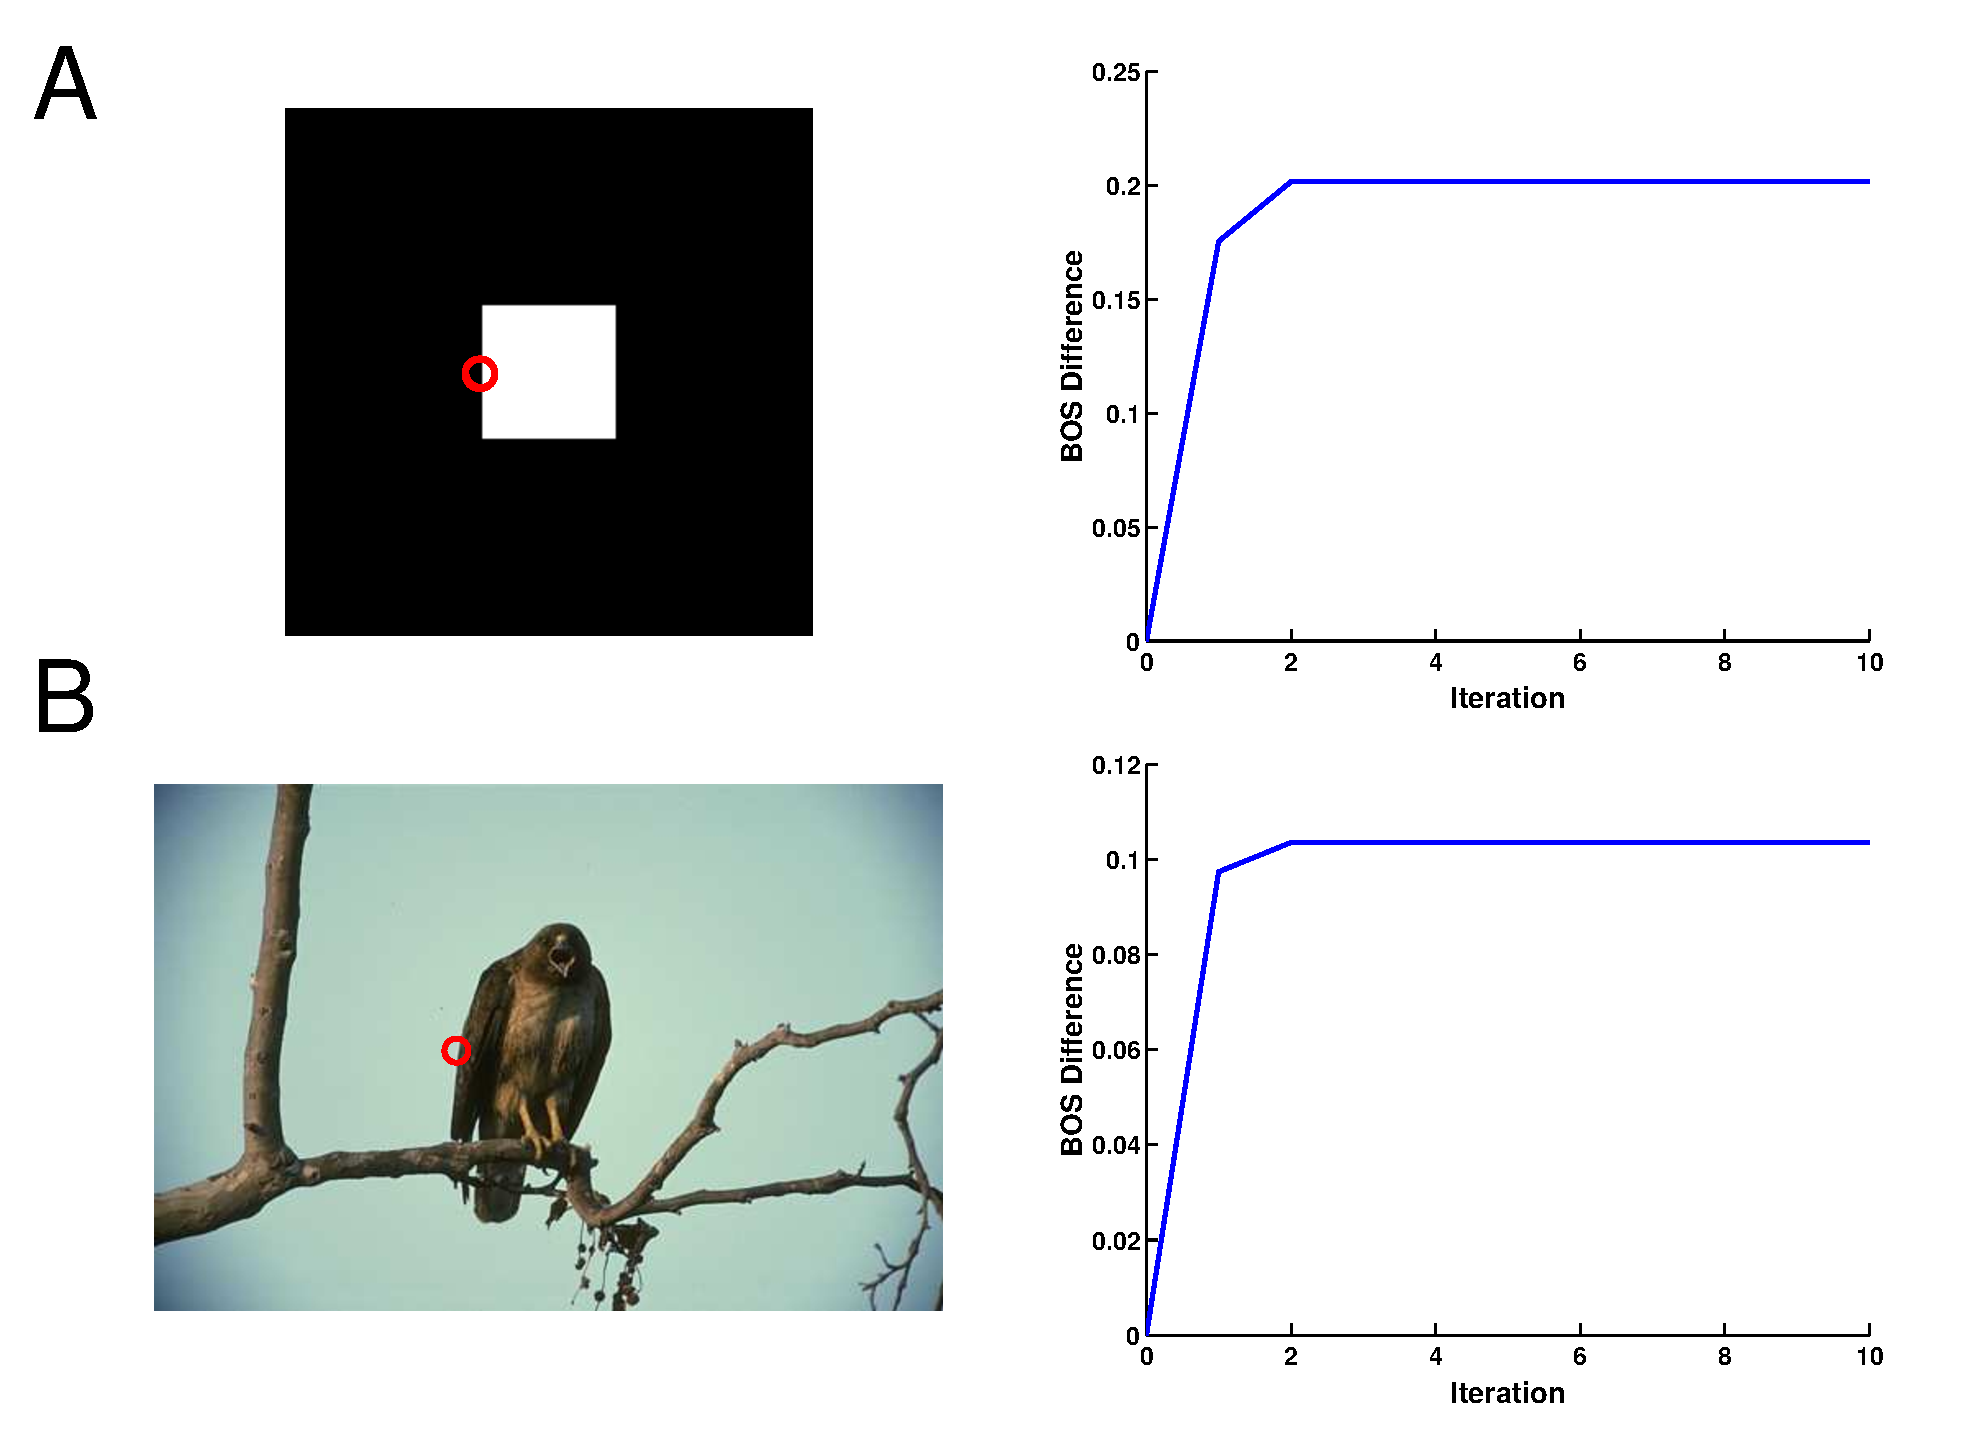
\includegraphics[width=\textwidth]{NaturalImage/figs/BOS_timecourse.eps}
\makeatletter
\let\@currsize\normalsize
% simplify caption
\caption[Time course of border-ownership coding]{Time course of border-ownership coding. The model converges to the correct border-ownership assignment within two-three iterations (one iteration corresponds to a feedforward and feedback pass through the model). The receptive field of the model's border ownership cell is shown by the red circle. The input image and time course of the border-ownership signal are shown for both the standard square commonly used in experiments (A) and an example natural scene from the Berkeley Segmentation Dataset (B). The border-ownership signal is computed as the difference in activity between the preferred and non-preferred border-ownership cells.}
\label{Fig:results_time}
\end{figure}

We report our results on the contour detection and figure-ground assignment tasks in Tables 1 and 2 above, respectively. All benchmarks were performed using public code made available by the authors of the original papers.

\begin{figure}[t!]
\centering
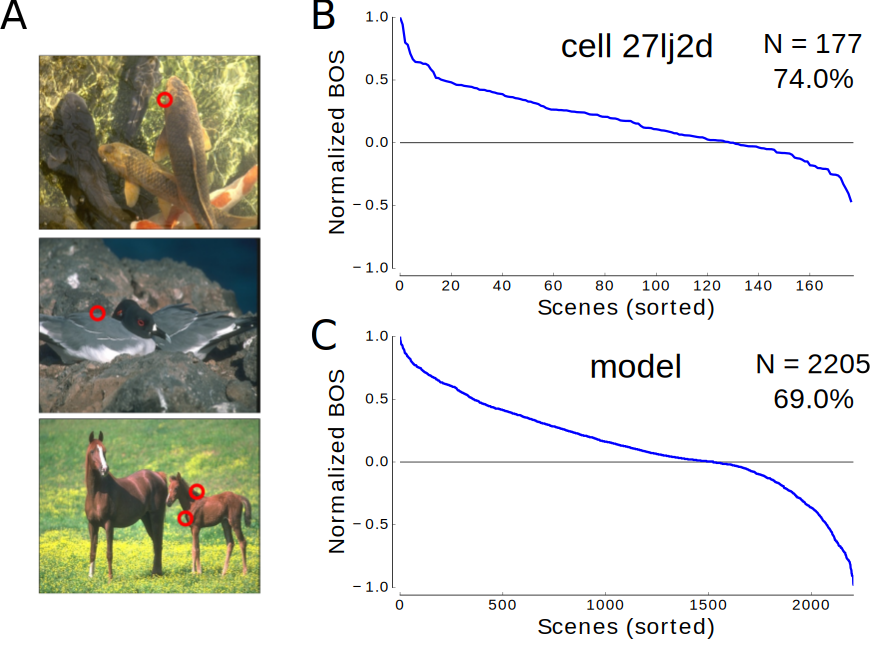
\includegraphics[width=\textwidth]{NaturalImage/figs/cell_model_consistency}
\makeatletter
\let\@currsize\normalsize
% simplify caption
\caption[Cell and model consistency across scenes]{Cell and model consistency across scenes. (A) Examples of scenes that were used to test border-ownership selectivity during the experiments. Red circles represent scene points within the images, which were centered on the receptive fields of border-ownership selective neurons during the experiments and during our testing of the model. A single image could contain multiple scene points, as shown by the example in the last row. (B) The normalized border-ownership signal (BOS) for example cell $27lj2d$ is shown according to each scene, with scenes sorted in decreasing order by strength of BOS. The cell achieved a consistency of 74.0\% across all tested scene points ($N = 177$). Consistency is defined as the number of scenes with positive border-ownership signal divided by the total number of scenes. (C) The normalized BOS signal for the model is shown with the same convention as in (B). The model achieved an overall consistency of 69.0\% across all tested scene points ($N = 2205$), consistent with our finding that the overall accuracy of the model is around 70\% on the figure-ground assignment benchmark.}
\label{Fig:cell_model_consistency}
\end{figure}


\subsection{Timing of the border-ownership signal}
% What other results would be nice to show?
We tested our model on both the standard square stimuli which are often used to determine border-ownership preference in experiments~\citep{Zhou_etal00}, as well as a wide array of natural scenes from the Berkeley Segmentation Dataset. We found that our model converges within a few iterations, demonstrating that only a few feedforward and feedback passes are needed to determine figure-ground assignment for a given image.
% more speculative here...
Given that white-matter projections in the brain are quite fast, we assume that a single feedforward and feedback pass in our model takes about 10 ms. As the model converges within 2-3 iterations, the border-ownership signal will reach its peak within 20-30 ms of the initial visual response. A similar time course has also been observed in the experimental data, with the border-ownership signal appearing approximately 30 ms after visual response onset~\citep{Williford_vonderHeydt16}.
%
The similar time course of BOS tuning on both artificial and natural stimuli points to a common cortical mechanism for grouping, which is also supported by previous experimental results demonstrating consistent border-ownership coding across different stimuli (Figure~\ref{Fig:results_time}).
% Can we comment more on the timing similarity with Jonathan's data?

\subsection{Comparison of model results to experimental results}
% Display figure here related to these results
The model exhibits consistent border-ownership coding across a large number of natural scenes. Figure~\ref{Fig:cell_model_consistency} compares the border-ownership signals sorted in descending order by scene for an example cell with that for the model. The example cell shows a consistency of 74.0\% across 177 scenes, which was the largest number of scenes that was tested for any single cell in the dataset. A large number of cells in the dataset were highly consistent, including the 13 cells we chose with $>$80\% consistency, and also 3 cells with $>$90\% consistency. In comparison, the model shows an overall consistency of 69.0\% across 2205 scenes, which is more than an order of magnitude more scnes than was tested on the example cell. This level of consistency is similar to the accuracy the model achieved on the figure-ground assignment benchmark, which was also close to 70\%.

We also used the cosine similarity metric to quantify similarity in BOS responses between cells and agreement between cells and the model on a shared set of scenes. Despite the large diversity of cells and their responses, we found that our model was able to largely explain the border-ownership coding of highly consistent cells on natural scenes. Figure~\ref{Fig:cell_model_cos} shows the cosine similarities for cell-model comparisons on a per-cell basis for the subset of highly consistent cells. The model-cell cosine similarities were all positive, ranging from 0.21 - 0.69, with a mean similarity of 0.44.

Given biological noise and inter-cell differences, we did not expect that the model-cell cosine similarities would reach 1. In order to characterize an upper bound on the cosine similarity values, we calculated the cosine similarities between all pairs of highly consistent cells($N = 58$ pairs). For the cell-cell comparisons, the cosine similarities ranged from 0.14-0.91, with a mean similarity of 0.54. Equivalence testing on the means of the cell-cell cosine similarities and model-cell cosine similarities revealed no differences in the mean values based on a zone of scientific significance of -0.2 - 0.2 ($p$ = 0.02). As a result, we conclude that our model performs similarly to the highly consistent cells in the dataset.

We also computed regression fits between the cell border-ownership responses and model border-ownership responses on a per-cell basis. Each regression outputs an $R^2$ value, which gives a measure of the percent of variance that the model is able to capture. The noise variance was estimated from the responses of each cell to a given scene and summed over the total number of scenes presented. The $R^2$ goodness of fit values ranged from 0.07-0.67. For two of the highly consistent cells, the $R^2$ measure exceed 0.5, indicating that the model was able to capturing over 50\% of the explainable variance.

\begin{figure}[t!]
\centering
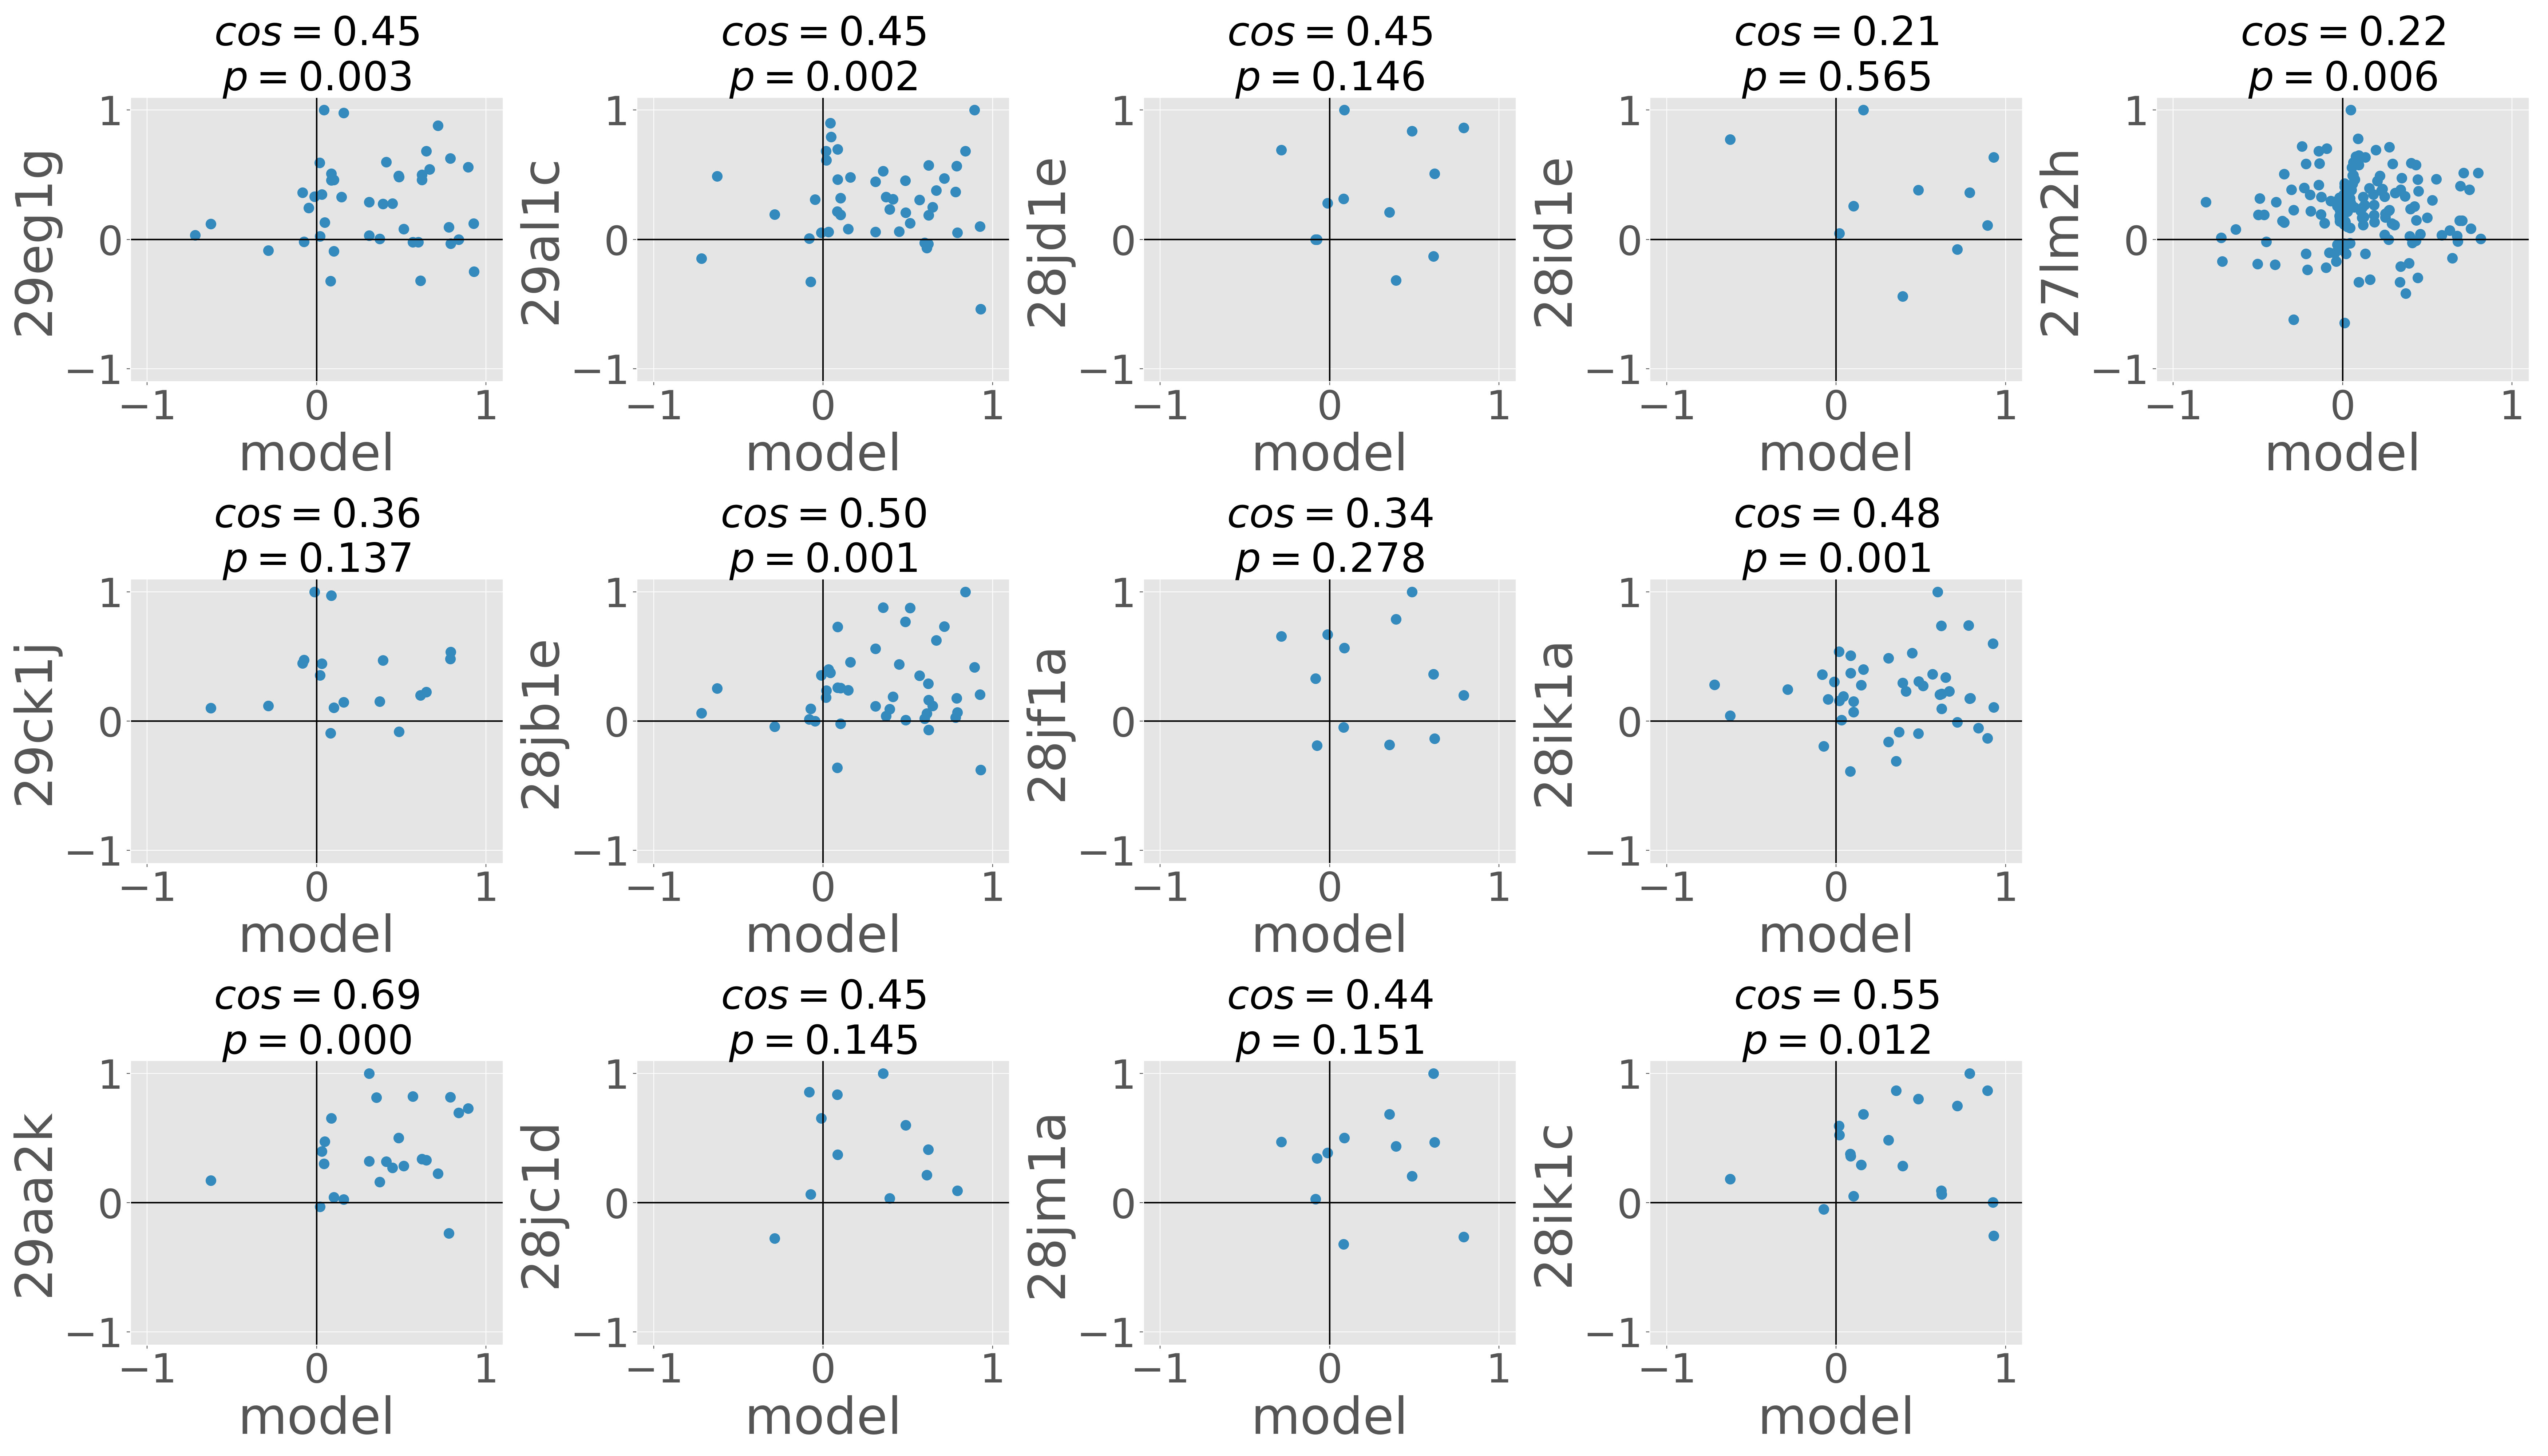
\includegraphics[width=\textwidth]{NaturalImage/figs/cell_model_cos_p}
\makeatletter
\let\@currsize\normalsize
% simplify caption
\caption[Cosine similarity between model and cell responses]{Cosine similarity metric comparing the model to the population of consistent cells. Each subplot shows a scatter plot of one cell's border-ownership signal against the model's border-ownership signal on the common set of scenes viewed by both. The cosine similarity metric along with the associated $p$-values (statistically different from a cosine similarity of zero) are shown above each scatter plot. Cosine similarities for the cell-model comparisons ranged from 0.21 - 0.69, with 7/13 cells having significant cosine similarities.}
\label{Fig:cell_model_cos}
\end{figure}

\section{Discussion}
\label{sec:discussion}

% bh First summarize the main results here:

%

\subsection{Understanding the cortical mechanisms of figure-ground organization}
% Explain how our model provides insight into the model, maybe list some testable predictions?
% Comment how a singular mechanism can explain BOS tuning, without requiring local cues like T,L junctions, etc
We propose that a simple grouping mechanism can explain figure-ground organization in natural scenes. Grouping cells in our model enforce the Gestalt principles of continuity and proximity with their annular receptive fields. Importantly, the design of these receptive fields was based on first principles, and not due to any training or parameter tuning on natural scenes, as is common in machine learning approaches. We show that this receptive field structure is useful for assigning figure-ground relationships in both artificial and natural stimuli. These receptive fields capture the convex shape of objects, which has been shown to be an important cue from the analysis of natural scene statistics~\citep{Sigman_etal01}. Our model does not rely on local cues, such as T-junctions and X-junctions, or higher-level object identity information, such as that from higher visual areas which may influence segmentation based on object familiarity. Instead, we propose that grouping in our model operates at intermediate levels of the visual hierarchy to structure the visual scene into proto-objects useful for further visual processing.

Our model border-ownership responses match the border-ownership responses of highly consistent cells from the experiments, which was tested by presenting the model with the same set of natural scenes as viewed by the cells. This is surprising given the diversity of cell responses to different natural scenes-- cells themselves are not entirely consistent with each other, perhaps indicating that a population of neurons is needed to accurately encode figure-ground relationships~\citep{Hesse_Tsao16}. However, our model, which is based on the simple principle of annular grouping cell receptive fields, is able to capture the responses of many of these neurons.
%
% Again, have to state more clearly how this is once we settle on a way to analyze the cell-model data
%
Furthermore, our model shows high accuracy across all tested scene points in a standard image benchmark dataset. We achieve an accuracy that exceeds 70\%, which is close to human performance on local boundary shapes derived from the same image dataset that we used~\citep{Fowlkes_etal07}. Humans achieve an accuracy of 68-69\% on this task. This suggests that the additional feedback connections in our recurrent model, which capture global context information about objects, may improve performance and may be helpful for figure-ground organization.

Our model relies on feedforward and feedback connections via fast white-matter projections between visual areas. This is consistent with the fast appearance of border-ownership signals after visual stimulus onset. This is a clear difference between our model and others which rely either on feedforward or lateral connections. We also use a variety of grouping cells of different scales, which allows our model to achieve relative scale invariance across the range of object sizes present in natural scenes. The main contribution of our present work is the development of a fully-image computable computational model of figure-ground organization that can be applied to natural scenes, which allows for further study of the potential cortical mechanisms of this process.

%
\subsection{Comparison to other models}
% Compare with previous figure-ground models
Many have argued that figure-ground assignment is purely local phenomenon
that only requires lateral connections
~\citep{Grossberg94, Grossberg97, Zhaoping05}. However, these models are largely untested on natural stimuli, and it remains to be seen if previous results on artificial stimuli will generalize to more difficult real-world conditions.
Our model is a member of a broad class of theoretical models that
achieve image understanding through bottom-up and top-down recurrent
processing~\citep{Ullman84,Hochstein_Ahissar02,Roelfsema_06,Epshtein_etal08}.
Our model is explicit in that feedback connections from higher visual areas
modulate the responses of early feature-selective neurons involved in
the related processes of contour integration and figure-ground
segregation. Despite requiring feedforward and feedback passes of information through
the model, our model converges quite quickly, consistent with the fast establishment of figure-ground relationships in visual cortex. 
%

% Compare with Sakai model
The only other model that has been tested on natural stimuli involved feedforward processing of asymmetric surround contrast~\citep{Nishimura_Sakai05,Sakai_etal12}.
% cite their 2012 paper?
In contrast to our model, their approach was not completely bottom-up (and hence, not fully image-computable). Instead, ~\citet{Sakai_etal12} tested model performance on human-labeled contours from the Berkeley Segmentation Dataset. Furthermore, their model was only able to use luminance information, so all images were first converted to grayscale. Our model is fully image-computable, which  means that it can be applied to any image, even those without human-labeled contours. Our model is also able to incorporate both luminance and color information from images, which allows it to be applied on a larger range of images and also to study the relative influence of these two cues for grouping.

Importantly, the two models also differ in their predictions about the role of feedback in figure-ground segmentation. One experimental prediction of our model is that disrupting feedback from higher visual areas (specifically, the feedback from grouping cells) would impair the figure-ground assignment process, and potentially result in poor border-ownership assignment and segmentation of objects in the scene. Models based purely on feedforward processing do not make this prediction. We also predict the existence of contrast-senstive and color-sensitive grouping cells, which send reciprocal feedback connections to similarly-tuned border-ownership cells.

\subsection{Grouping neurons}
% List possible feature extensions of the model
% List hypothesis of grouping neurons
There is no clear neurophysiological evidence for
grouping neurons yet,
although previous studies have found neurons in V4 
that respond to contour segments
of various curvatures~\citep{Pasupathy_Connor02,Brincat_Connor04}. The receptive fields of these neurons are
similar to those proposed in the model by
\cite{Craft_etal07}. Other types of grouping neurons may also exist,
including those that respond to 
gratings~\citep{Hegde_vanEssen07}, illusory
surfaces~\citep{Cox_etal13}, or 3D
surfaces~\citep{He_Nakayama95,Hu_etal15a}.
We do not attempt to model the whole array of grouping neurons that may exist, but
only those necessary for reproducing figure-ground assignment in natural scenes. Furthermore, grouping neurons may be cross-modal, in that they respond to different features that may aid the scene segmentation process, such as disparity, motion, \etc. In fact, experimental results show that border-ownership selective neurons have consistent border-ownership tuning across 2D luminance and 3D disparity cues~\citep{Qiu_etal05}. We have not yet incorporated these additional features into our model, but this represents a potential future area of research.

\subsection{Scope and limitations of the model}
% List limitations of the model, list future directions/applications of model
% No fine-scale time dynamics, for understanding synchrony etc.
Our model assigns distinct roles to the
different visual areas,  \eg edge processing in V1 by simple cells, figure-ground
assignment in V2 by border-ownership selective cells, and grouping of objects in V4. However,
the physiological properties of neurons in early visual areas have not
been fully characterized, and 
neurons in these different
areas may have 
additional ranges of selectivity
than the ones we assign them in our model. 
Our model also produces a rough approximation of the time course of border-ownership
coding through a discrete iterative process. As such, it does not allow us to study the dynamics of the recurrent network at a finer time scale. For example, the synchrony between border-ownership neurons that are part of the same object is of particular interest~\citep{Martin_vonderHeydt15,Wagatsuma_etal16a}. Furthermore, we focused more closely on the border-ownership cell activity in our model and did not specifically study the grouping cell responses of our model, but the combined activity of grouping cells across cells can be used to
study a wide range of other visual phenomena, including object segmentation and visual saliency.

%%% Local Variables:
%%% mode: latex
%%% TeX-master: "../root"
%%% End:
%\chapter{3D Surface Representation}
\label{sec:surfaces}
\chaptermark{3D Surfaces}

\section{Introduction}
Since we live in a complex 3D world, competent interaction with the
surrounding 3D scene structure is indispensable to us and our machines. Access to information about surfaces present in the scene allows us to perform a wide variety of tasks, ranging from motor planning (\eg reaching for a cup a certain distance away on the table) to spatial navigation (\eg following directions in a new city environment).

%While it may be tempting to believe that only "higher" organisms need to have a representation of 3D scene structure, similar abilities have also been found in much "simpler" animals. For example, jumping spiders hunt for prey in complex 3D environments. Their behavior consists of first analyzing the 3D surface layout of the environment before planning and executing a route to their prey. Jumping spiders must keep track of their movement goal despite large changes in their own position within the 3D environment, pointing to a stable and persistent surface representation. These studies illustrate that the representation of surfaces within 3D scenes may be an ecologically important function, conserved across many different animal species and adapted to their own natural environments.

In studying perceptual organization, researchers have traditionally
relied on simple 2D stimuli such as oriented bars~\cite{Palmer_02}. Results from these studies provide support for the importance of well-known Gestalt principles~\cite{Koffka35, Wertheimer23}, for instance that visual elements are grouped together in a way that begins to give meaning to the visual scene (\eg figure \vs background). However, it is unclear how well the results from these relatively simple experiments generalize to the 3D objects and scenes regularly encountered in natural settings. Because we act in a 3D world, perceptual organization must also help to arrange 3D information in a way that can guide our actions. 

Perceptual organization also provides a structure for selectively
attending to groups of objects~\cite{Treisman_Gelade80}. Supported by
extensive psychophysical data, Nakayama, He, and Shimojo~\cite{Nakayama_etal95} proposed that surface representations
play a key role in intermediate-level vision. For example, by selectively attending to a surface in 3D space, subjects can perform
efficient search for a conjunction target~\cite{Nakayama_Silverman86}. In a separate cueing experiment, attention was shown to spread automatically across surfaces~\cite{He_Nakayama95}. These abilities indicate powerful mechanisms for grouping objects into surfaces in 3D space, and suggest that structuring the world in terms of surfaces might be an ecologically important function. These results also have implications for the internal representation of surfaces, because they imply that the visual scene is processed in a way that preserves its 3D
structure. This representation must also be able to bring together
information from different sensory modalities (\eg vision, audition,
\etc), in order to form a common representation of the 3D environment
that is useful for an agent's behavioral goals~\cite{Lewicki_etal14}.

In addition to being studied by human psychophysical approaches, perceptual organization has been the subject of many studies in the
visual system of non-human primates. Many neurons in early visual cortex encode the side to which an object border belongs, a phenomenon known as border ownership~\cite{Zhou_etal00}. Selectivity for the side of ownership involves integrating global context information about the
object. Several models have been proposed~\cite{Zhaoping05, Craft_etal07} to describe how a neuron's border ownership selectivity can be modulated by visual input far away from its classical receptive field with the observed high specificity of object details. One view is that this contextual input is provided by feedback connections from ``grouping cells''~\cite{Craft_etal07} which bias the activity of border ownership cells and thus generate their context-dependent responses. Mihalas et al.~\cite{Mihalas_etal11b} have also shown that
grouping cells can direct and sharpen a broad attentional spotlight to
the lower-level features of a specific object. In the present study, we extend this grouping framework to 3D space to show how oriented 3D
elements can be grouped into planar surfaces.

Currently, we know very little about how surfaces are represented in
the brain, and how this representation is computed.  Our model sheds
light on a possible neural representation of 3D surfaces and relates
this model to previous psychophysical results.

\begin{figure}[t]
\centering
\includegraphics[width=3 in]{3D-Surface/figs/groupingcircuit}
\makeatletter
\let\@currsize\normalsize
\caption{Network structure (adapted from ref.~\cite{Marshall_etal96}).}
\label{NetworkStructure}
\end{figure}

\section{Methods}
An overview of the network structure of our model is shown in
Figure~\ref{NetworkStructure}. We extend a neural model of visual
stereomatching~\cite{Marshall_etal96} that is conceptually similar to
grouping models previously proposed for 2D stimuli~\cite{Craft_etal07, Mihalas_etal11b, Russell_etal14}. The model contains three layers of neurons. The first layer consists of monocular cells, which respond to visual features (e.g. spots, edges, {\em etc.}) presented to either the left or right eye. The input to the model consists of pairs of stereo images, as would be seen by the left and right eyes. In our model, we set the image input to a value of unity wherever a stimulus is present and zero elsewhere.

The second layer consists of binocular cells, which receive excitatory
input from monocular cells. These cells are tuned to a certain disparity based on a fixed spatial weighting between the left and right monocular cells, analogous to the disparity-selective binocular neurons in visual cortex of monkeys~\cite{Poggio_Fischer77, Poggio_Poggio84} and cats~\cite{Bishop_Pettigrew86, Ohzawa_etal90}. Lateral inhibition between cells representing different disparities along the same left- or right-eye line of sight reduces potential false matches~\cite{Marr_Poggio76}.

The third and final layer consists of planar grouping cells which receive excitatory input from populations of disparity-selective
cells. Receptive fields of the planar grouping cells are relatively broad and non-specific, resembling surface patches with a certain range of depth and orientation selectivity in 3D space. These cells may correspond to neurons found in parietal cortex, which have been shown to be selective for the tilt and slant of planar surfaces~\cite{Rosenberg_etal13}. In our model, we used a total of 15~planar grouping cells, which was sufficient to ``tile'' the whole 3D visual scene. Planar grouping cells compete with each other through lateral inhibition, which helps to select the best possible interpretation of surfaces within the scene. Additionally, planar grouping cells send reciprocal feedback connections to the disparity-selective cells that define their surface, akin to the relationship between grouping cells and border ownership cells in
models of 2D scenes~\cite{Craft_etal07,Mihalas_etal11b}. To avoid
uncontrolled feedback excitation, feedback is multiplicative and only amplifies existing feedforward excitation. Selective attention is modeled as an additive input to those planar grouping neurons representing attended objects. This attentional modulation input is set to a value of 0.25 of the sensory input.

All model neurons are simulated as single compartment units with an
activity that is modeled as a continuous variable (rate coding). These
units are zero-threshold, linear neurons which receive excitatory and
inhibitory current inputs. The activity of the units is determined by
a set of coupled, first-order nonlinear ordinary differential equations, which can be solved in MATLAB (MathWorks) using standard numerical integration methods (Euler, Runge-Kutta, \etc) 

\begin{figure}[t]
\centering
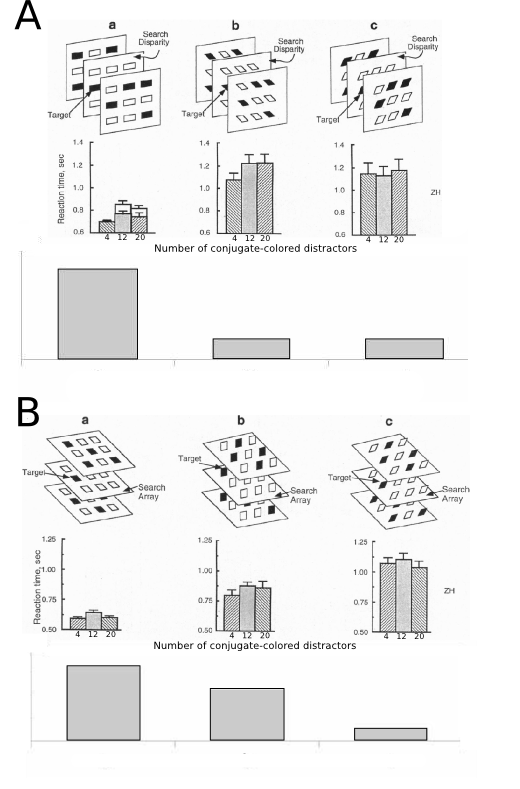
\includegraphics[width=3in]{3D-Surface/figs/nakayama}
\makeatletter
\let\@currsize\normalsize
\caption{Psychophysical and model results (adapted from ref~\cite{He_Nakayama95}). For each trial type (A or B), the top row shows the different stimuli, the middle row shows representative reaction times, and the bottom row shows the degree of attentional modulation of disparity-selective cells on the  attended plane. Increase in activity is assumed to be inversely proportion to reaction times.}
\label{ModelResults}
\end{figure}

\section{Results}
Figure~\ref{ModelResults} illustrates the experimental paradigm of He
and Nakayama \cite{He_Nakayama95}. In Figure~\ref{ModelResults}A, subjects had to search for the odd-colored target in the middle depth
plane; planes are outlined by rectangles that were not visible to the observers. The target was unique in this search plane but visually identical distractors  were present in other depth planes. In A-a, objects are aligned with the search plane while in A-b and A-c, they are slanted out of the plane. The middle row in A shows measured reaction times for three different numbers of distractors.They are significantly shorter when the objects are coplanar with the search plane (A-a) compared to when they are not aligned with the plane (A-b and A-c).

\begin{figure}[t]
\centering
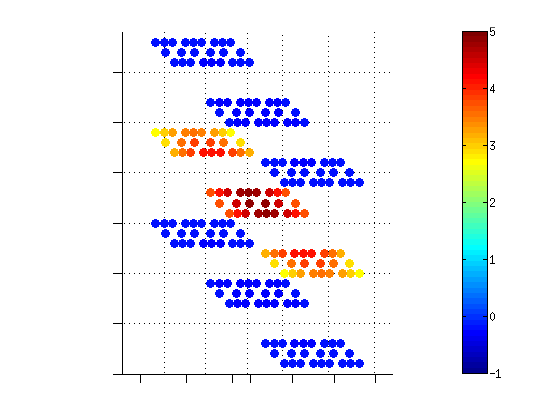
\includegraphics[width=3in]{3D-Surface/figs/attentionmod}
\makeatletter
\let\@currsize\normalsize
\caption{Spread of attention across surfaces. When attention is directed to the center slanted plane (as in the experiment in Figure 2B-a), attention enhances the activity of all cells along the surface (red), while suppressing the activity of cells belonging to other surfaces (blue).} 
\label{ModelResults2}
\end{figure}

In our model, we assume that the visual system can selectively direct
attention towards a specific surface by providing additional excitatory input to the grouping cell that represents this surface. As shown in Figure~\ref{NetworkStructure}, activity from the grouping cell selectively feeds back to all objects on that surface. In the case of Figure~\ref{ModelResults}A-a, the grouping cell corresponding to the middle fronto-parallel plane receives this attentional input. 
Activation of the disparity-selective cells in the search plane, shown in Figure~\ref{ModelResults}A-a, bottom row, is thus high. Among the objects in the search plane, the target has a unique color, which results in efficient search and the target being identified immediately. Reaction times are difficult to simulate in detail, therefore the increase in mean activity of disparity-selective cells on the attended plane due to attentional modulation is plotted instead,
which is assumed to be inversely proportional to reaction times. The
high activation level, bottom row, translates thus into short reaction
times, middle row.

In contrast, in Figure~\ref{ModelResults}A-b, the search plane is no longer a well-formed surface but contains objects that are slanted
backwards. Directing attention to the middle fronto-parallel plane
then has little effect on the disparity-selective cells in the search
plane. Search therefore cannot occur entirely within a single plane of coplanar, grouped elements and becomes inefficient, with much higher reaction times (middle row). These long reaction times are reflected in the low activation level of the disparity-selective cells (bottom row). Figure~\ref{ModelResults}A-c shows the analog result for figure elements that are slanted forward rather than backwards, as in A-b. Again, reaction times are long and population activity is low. 

The result is not restricted to fronto-parallel planes, as similar reaction time results were also found for slanted planes in Figure~\ref{ModelResults}B. When subjects are instructed to search in
a plane that is coplanar with the orientation of the figure elements
(middle plane in B-a), search is fast (B-a, middle row). In contrast,
when the figure elements do not align with the search plane (top row in B-b and B-c), reaction time is increased (middle row). Again, under the assumption that reaction times are inversely related to reaction times, the model reproduces human behavior (bottom row).

Attention to grouping neurons is then able to select sets of objects
organized in planes. Reaction times were fastest when the search array was a well-formed surface defined by locally coplanar elements. When search array elements were slanted away from this surface, reaction times increased. These results suggest that attention is linked to and spreads across perceived surfaces, which organize the visual scene
(Figure~\ref{ModelResults2}). 

\section{Conclusion}
Using a simple model of perceptual organization in 3D,  we are able to reproduce psychophysical results from a visual search task that required allocation of selective attention to surfaces within the scene. The same grouping cells which organize the scene into planes also act as ``handles'' for top-down selective attention, enhancing the activity of coplanar elements belonging to the plane. Competition between grouping cells results in surface enhancement of the plane
corresponding to the attended grouping cell, and suppression of other
planes within the scene. Our proposed surface representation aids visual processing by providing a critical link between low-level
visual features and high-level object representations.
%\chapter{3D Proto-object based Saliency}
\label{sec:saliency}
\chaptermark{3D-Saliency}

\section{Introduction}
The brain receives large amounts of visual information that it must make sense of in real-time. Processing the entire visual field with the same level of detail present at the fovea would be an exceedingly complex and costly task requiring much greater computational resources than are available~\citep{Tsotsos90}. As a result, primates select only the most relevant information and discard the rest, a process known as selective attention. Visual attention is controlled by both bottom-up and top-down mechanisms, which interact to influence the organism's behavior~\citep{Yarbus67}. Bottom-up attention is involuntary and signal-driven, largely due to the fact that some stimuli are more conspicuous and able to stand out from their surroundings. Top-down attention is task-dependent, and can take into account semantic information such as the familiarity or interestingness of an object, which biases the organism's attention based on its internal state or goals.

Many models of visual attention are constructed with a bottom-up architecture and rely on local contrast in low-level features such as
intensity, color, orientation, or motion. Biologically-plausible
center-surround differences across different feature channels of an input image can be used to compute a ``saliency map'' whose maxima
indicate where selective attention is deployed \citep{Koch_Ullman85,Niebur_Koch96b,Itti_etal98a}. However, there is
both psychophysical~\citep{Einhauser_etal08a} and neurophysiological~\citep{Zhou_etal00, Qiu_etal07} evidence that attention relies not only on these simple image features, but also on
the perceptual organization of the visual scene into tentative objects, or proto-objects~\citep{Rensink00a}. A biologically-inspired model of proto-object based saliency has been proposed to take into account these recent findings \citep{Craft_etal07,Mihalas_etal11b,Russell_etal14}. The model includes border ownership selective cells (referred to as border ownership cells in the following) and grouping cells, which interact to achieve figure-ground segmentation of the image into proto-objects (figures) and the background (ground). Border ownership cells have been found in primate visual cortex, with the majority of neurons in area V2 having this property. These cells signal in their neural activity the one-sided assignment of an object border to the region perceived as figure \citep{Zhou_etal00}.  Border ownership cells are also modulated by attentional influences \citep{Qiu_etal07}. Grouping cells integrate global context information about proto-objects in the scene according to Gestalt principles such as closure, continuity, convexity \etc Importantly, grouping cells act at intermediate stages of vision and do not require higher-level information about object identity, semantic knowledge \etc They send feedback to border ownership cells \via fast white matter projections, which bias the activity of border ownership cells to reflect the correct figure-ground segmentation of proto-objects. In this framework, visual saliency is a function of grouping cell activity, which represents the size and location of proto-objects within the image.

Border ownership cells have been shown to respond to figure edges defined by a variety of image features, \eg luminance edges, color
edges \etc When no monocular edge information is present (\ie when the
figures are defined by random dot stereograms using only binocular
disparity), border ownership selectivity is also imparted by stereoscopic edges~\citep{Qiu_vonderHeydt05}. Critically, their response to these different figural cues is typically the same in the two-dimensional (2D) and three-dimensional (3D) cases -- the preferred side-of-figure of border ownership cells is consistent for all cues that define the figure. The activity of border ownership cells thus provides an interpretation of the visual scene in terms of depth-ordered surfaces that correspond to objects in 3D space. 

In a separate line of work, it has been shown that surface representations play a key role in intermediate-level vision, and that
visual attention can be deployed at the level of perceptual surfaces
\citep[][for a model of attention to surfaces see Hu \etal 2015]{He_Nakayama92,He_Nakayama95}.\nocite{Hu_etal15a} Despite these experimental observations, current models of border ownership do not explicitly use depth information and do not address how traditional 2D Gestalt cues interact with depth cues during the figure-ground segmentation process. An exception is a study by~\cite{Mishra_etal12} who used computer vision methods to compute border ownership from low-level depth information and then performed object segmentation in natural images.

Even though in recent years stereoscopic 3D content has become increasingly prevalent, \eg in the viewing of entertainment programs
in cinemas and homes, little is known about how visual attention is
deployed within 3D environments.  It is thus important to understand
how humans allocate their attention when viewing natural images and
videos in 3D \citep{LeCallet_Niebur13}. Binocular disparity cues, which can be used to generate strong depth percepts, have been shown to alter different aspects of eye movements when participants viewed 3D images~\citep{Jansen_etal09} and videos~\citep{Huynh_Schiatti11}. Only recently have 3D eye tracking datasets been made available which can be used to compare human eye movements with predictions of attentional models. The availability of these datasets and the recent explosion in new 3D content makes it possible to design computational models of 3D saliency and evaluate their performance objectively.

The goals of our research are (1)~to extend a proto-object based saliency model \citep{Russell_etal14} to include depth information, and (2)~to evaluate its performance in perceptual saliency prediction. We show that combining 2D Gestalt cues with depth cues improves the performance of our model on three different 3D eye tracking datasets. In the model, depth information along with other 2D features biases grouping cell activity, which then interacts with border ownership cells to represent proto-objects, the tentative objects within the scene. These proto-objects are a first step in figure-ground segmentation of the image, and also give an indication of the salient points within the image. We evaluate the proto-object saliency maps produced by our model against ground truth data in the form of human eye fixations using a battery of different metrics.

\section{Related Work}
\subsection{Models of 3D visual attention}
Compared to the number of models that have been proposed for 2D visual
saliency, relatively few attempts have been made to study how visual
attention is deployed within 3D environments. Existing models of 3D
visual attention often compute a 2D saliency map which is then combined
with the depth information to produce a new saliency map. These models
fall into three categories~\citep{Wang_etal13} based on how the depth
information is used: stereovision models, depth-weighting models, and depth-saliency models. For a comprehensive review of 3D visual attention models, see~\cite{Wang_etal13,Ma_Hang15}.

While the depth-weighting and depth-saliency models assume that a depth map has been computed, without specifying how, stereovision models explicitly implement the computation of depth information from
the left and right views of the scene, thus replicating the human visual system's stereoscopic perception.  An example of this is a
study by~\cite{Bruce_Tsotsos05}, which extended a 2D selective tuning
model of attention to also incorporate binocular information. However,
no quantitative assessment of this model was performed.

Depth-weighting models use a base 2D saliency model (computed using one of the existing methods) and then multiplicatively weight the
resulting saliency map with the depth information. Regions that are
closer to the observer obtain higher weights, corresponding to greater
combined saliency. In a model developed by~\cite{Lang_etal12}, novel
depth priors are learned from a training portion of the data, and these are then combined with the output of a 2D saliency model either
using pixel-wise addition or multiplication. With these depth priors,
the authors find an increase of performance by 6-7\% on their dataset
compared to the base 2D model without depth information.

Depth-saliency models come in two flavors. In one, both a depth saliency map, obtained from depth alone, and a more traditional saliency map, obtained from 2D information alone, are computed. The two
maps are then linearly combined to generate the final saliency map. \cite{Wang_etal13} determine depth saliency in a separate experiment involving synthetic stereoscopic stimuli, which allows them to reduce the influence of monocular depth cues, as well as control for the depth of objects and the background. With their experimental results, they propose a probabilistic model of depth saliency, where the probability of a point being fixated in 3D space is related to the
magnitude of center-surround differences in depth contrast. Linearly
combining these two saliency maps in a 1:1 ratio (50\% weight each for
2D features and depth information) results in better performance on
their dataset. In the second type of depth-saliency models, depth
information is treated as an additional feature channel, on the same
footing as intensity, color, orientation \etc The final saliency map is then a function of depth as well as of these other features \citep{Ouerhani_etal00,Jost_etal04,Hugli_etal05}.

Our approach falls in the latter class of depth-saliency models, where
all image features, including depth, interact through linear combination resulting in the final saliency map. Our model is completely integrated -- depth information is treated as another cue
which interacts with 2D Gestalt cues to influence figure-ground assignment of proto-objects within the scene. This agrees with anatomical and neurophysiological data that show that disparity selective cells, which are important for encoding stereoscopic depth
information, are found in the same early cortical areas as neurons representing other features used in typical saliency models, like
color and orientation \citep{Hubel_Wiesel62,Poggio_etal88b}. Different
from previous models \citep{Ouerhani_etal00,Jost_etal04,Hugli_etal05},
our model is not only based on basic image features (like color, intensity \etc) but it includes elements of perceptual organization, in particular proto-objects. The model is an extension of a previously
described 2D model \citep{Russell_etal14} and is constructed by including depth information as an additional feature. All features are used to determine proto-object based saliency.

We tested our model on the three 3D eye tracking datasets listed in the next section, and we compared results with and without the added
depth information.

\subsection{3D eyetracking datasets}
A common method for evaluating the quality of computational models of
visual attention is to compare their performance in the prediction of
human eye movements. Since its introduction by \cite{Parkhurst_etal02a}, this method has been used in a large number
of studies, both for static and dynamic scenes (video) and both for
human and non-human primates \citep[for a recent review see][]{Borji_Itti13}.  Nearly all of this work has been limited, however, to 2D scenes.

In order to evaluate 3D  attention models, eye tracking data on a variety of visual scenes have to be collected. We use  datasets  of natural images consisting of color images and associated depth maps along with human fixations for each image.  Predictions of saliency maps for eye movements can then be compared to the ground truth fixation data using various metrics. Below, three such publicly available datasets are described. Figure~\ref{Fig:Results} shows one example of the data available from each of them. 

\begin{figure}[htbp]
\centering
\includegraphics[width=6in]{3D-Saliency/figs/Results_Fig.eps}
\makeatletter
\let\@currsize\normalsize
\caption{Examples of data used and results obtained. Columns (left to right) show one example each of the original image with its corresponding depth map, fixation map, our saliency model without ($S$) and with ($S_d$) depth information for the three 3D eye tracking datasets: a) NUS-3D. b) Gaze-3D. c) NCTU-3D.}
\label{Fig:Results}
\end{figure}

The NUS-3D dataset~\citep{Lang_etal12} contains 600 RGB and depth image pairs, each with a resolution of $640\times480$ pixels. The images show various scenes around the National University of Singapore
(NUS) campus and were collected with a Microsoft Kinect camera, which
is capable of recording both RGB and depth images. The Kinect depth sensor is affected by ambient lighting and has a depth range of only
about 4~m, which restricts the types of scenes it can accurately capture. The images were presented to 80 participants and each participant's eye tracking data was captured in both 2D and 3D free-viewing experiments. The 3D stimuli were generated by virtual view synthesis \cite[see][for details]{Lang_etal12} but the synthesized 3D images are not available to the public. Only the raw
and smoothed depth maps from the Kinect as well as the fixation density
maps for the 2D and 3D viewing conditions are available.

The Gaze-3D dataset~\citep{Wang_etal13} consists of 18 stereoscopic
images, along with their associated disparity maps and perceived depth maps \cite[perceived depth is computed from raw disparity by taking into account viewing distance and display properties; see][for details]{Wang_etal13}. The ground truth disparity maps were calculated
from separate left and right image views using an optical flow method~\citep{Werlberger_etal09}. The images come from the Middlebury
2005/2006 stereo image dataset~\citep{Scharstein_Pal07} and the IVC 3D image dataset~\citep{Urvoy_etal12}. The dataset also contains raw eye tracking data for both the left and right eyes, as well as processed fixation density maps from a total of 35 participants. The images are high resolution ($1300\times1080$ pixels for the Middlebury subset and $1920\times1080$ pixels for the IVC subset) and have relatively accurate depth information. A limitation is the small number of images
in the dataset.

The NCTU-3D dataset~\citep{Ma_Hang15} consists of 475 2D images with a resolution of $1920\times1080$ pixels along with their corresponding depth maps and eye tracking data. The eye tracking data is in the form of fixation density maps and binary fixation maps. The images in the dataset were collected from randomly selected frames extracted from 11 different sequences of 3D videos from either Youtube (youtube.com) or 3dtv (3dtv.at). The depth maps were generated from left and right eye views using Depth Estimation Reference Software (DERS; version 5.0). A total of 16 participants freely viewed the videos in 3D.

\section{Model}
Our approach is based on the proto-object based saliency model proposed by \cite{Russell_etal14}. In the model, grouping cells group visual features into proto-objects that are characterized by their locations and spatial scales. The large annular receptive fields of the grouping cells enforce the Gestalt principles of closure and convexity, which in turn biases the activity of proto-objects towards the center of objects. Proto-objects are then a means to organize the scene into separate figures as well as the background. The grouping mechanism operates on multiple feature channels and incorporates competition between proto-objects of similar size and feature type. The model explains the development of border ownership findings in primate cortex \citep{Craft_etal07,Zhou_etal00}. Given that human eye movements tend to fall predominantly on objects \citep[][ but see \cite{Borji_etal13} for a different view]{Einhauser_etal08a}, which are often closed and convex, the locations of proto-objects are also assumed to correlate with the salient points within the image. For a full description of the original model, we refer the reader to \cite{Russell_etal14}.

We extend this model to include depth information. Since some images have border artifacts, all images are cropped to avoid spurious model responses at the borders. To achieve scale invariance, we create an image pyramid spanning 8-10 octaves (depending on the size of the image) by successively down-sampling the input image in steps of 2. We use a minimum cut-off image size of $3\times 3$ pixels, such that pyramid levels that would reduce the image size below $3\times 3$ pixels are not included in our model. All operations are applied independently to each feature and at each level of the feature pyramids, except for when the scales and features are combined to obtain the final saliency map. Each layer of the network represents the neural activity of an array of neurons which tile the visual scene and  which are propagated to other layers in the network through feedforward connections. The receptive fields of neurons are described by different correlation kernels, and the image input to each neuron in the model is calculated using the correlation operation. The model was implemented using MATLAB (Mathworks, Natick, MA). A model overview is shown in Figure~\ref{Fig:Model}.

\begin{figure}[t]
\centering
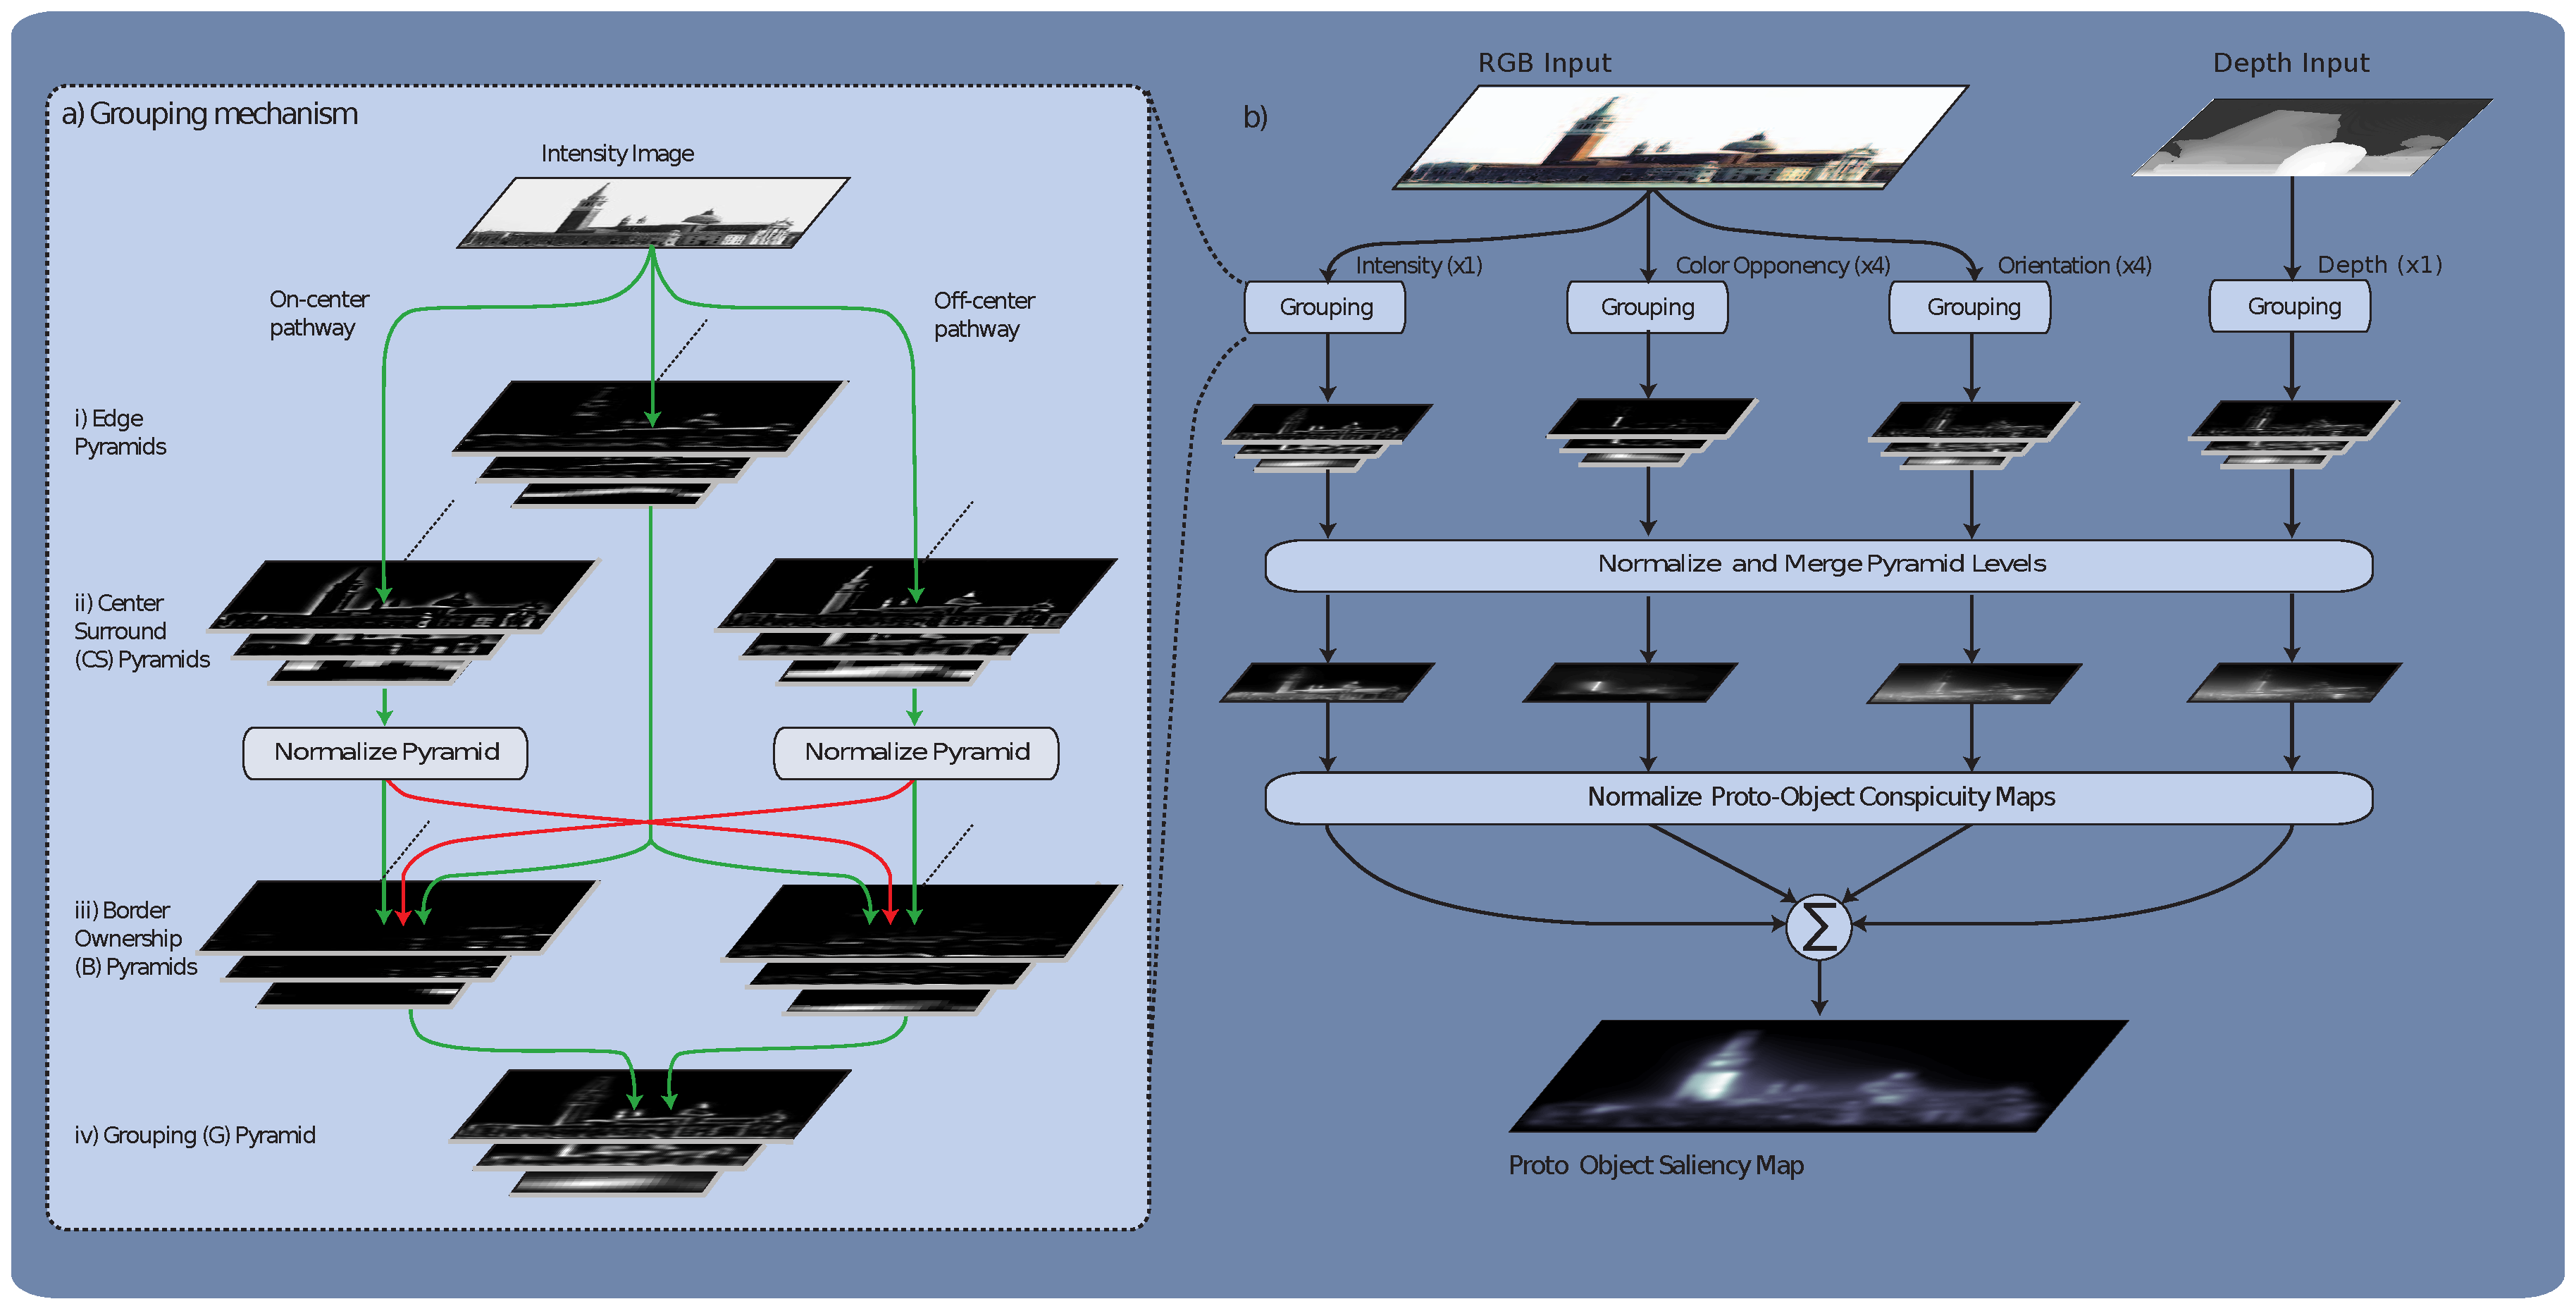
\includegraphics[width=6in]{3D-Saliency/figs/DepthSaliency_new1.eps}
\makeatletter
\let\@currsize\normalsize
\caption{Proto-object saliency model with added depth information. The depth map is represented by the image at the top, far right, and the 2D image is to its left. Based on Figure~5 of \cite{Russell_etal14}.}
\label{Fig:Model}
\end{figure}

In this report, we will refer to the saliency map generated by the
original 2D model without depth information as $S$, and to the saliency model generated by our new model, which incorporates depth
information as $S_d$. To compute $S$, the model accepts an input RGB
image and decomposes it into different feature channels: one intensity
channel, four color-opponency channels, and four orientation channels.
Rather than providing ``raw'' stereoscopic disparity information in the form of different images to the two eyes (or retinae), we assume
that the transformation from disparity information to depth has been
performed at the input level to our model. There is well-known neuronal circuitry that transforms stereoscopic disparity into depth
information \cite[\eg][]{Poggio_Poggio84} and the explicit representation of depth is more appropriate for the intermediate-vision conceptual level of our proto-object based model
than the ``raw'' representation in terms of binocular disparity. Therefore, to compute $S_d$, we add an additional depth feature channel obtained from the input depth image. Within each feature channel, we perform edge filtering (using oriented Gabor filters at 4 orientations) to obtain the location of proto-object borders. In order
to perform feedforward computation of figure-ground segregation, we
employ a center-surround mechanism, similar to that used by \cite{Itti_etal98a}; such mechanisms have been observed at multiple
stages in the brain, including retina, lateral geniculate nucleus, and
cortex (\ibid). This center-surround mechanism provides context information about proto-objects, and biases the activity of border-ownership cells with preferred directions that match the location of the figure.

For the 2D features used in our model, the center-surround mechanism
is symmetric with respect to figure-ground contrast polarity (\eg
light figures on dark backgrounds or dark figures on light background
result in the same net salience contribution). In contrast, for the
depth channel we compute the center-surround differences in an asymmetrical manner, consistent with the kind of information provided by stereoscopic depth.  While most feature differences across a contour are not predictive about which of its sides is the foreground\footnote{Exceptions are T-junctions \citep{Heitger_vonderHeydt93} and extremal edges \citep{Palmer_Ghose08,Ramenahalli_etal11a,Ramenahalli_etal12a,Ramenahalli_etal14a} both of which are local cues that provide information about edge polarity.\label{EEfootnote}}, stereoscopic depth (disparity)
provides nearly unambiguous information about which side of the border
is closer to the observer. This side ``owns'' the object border when
considered in a depth ordering sense and is part of the foreground. Physiological data show that the responses of border ownership cells to disparity differences across a figure edge are in agreement with this observation \citep{Zhou_etal00,Qiu_vonderHeydt05}. Therefore, in our model near \vs far depth differences bias the activity of border ownership cells such that the near side is more likely to be classified as the foreground object.  Integrating depth information into the representation of an object by its contours is a critical difference between our model and other depth saliency models which
directly combine depth feature information with 2D information, without taking into account perceptual grouping effects \cite[\eg][]{Ouerhani_etal00,Jost_etal04,Hugli_etal05}.  By modeling
the response of border ownership cells to depth edges, we enforce an
additional constraint on how depth information is to be combined with
2D information in order to produce proto-objects and the resulting salient points of the image.

Each channel is processed independently of the others by the same
grouping mechanism, and then combined through a series of normalization operators, which allow for competition between proto-objects of similar scale and feature. The final feature map is
obtained by scaling each map to a common scale (approximately the middle level of the image pyramid), and then performing a pixel-wise
addition across scales. The different feature conspicuity maps are then normalized again and linearly combined with equal weights to form
the proto-object saliency map $S$. When depth information is used, we
use a linear combination of 80\% 2D features, split equally among
intensity, color, and orientation, and 20\% depth features to form the
depth-added proto-object saliency map $S_d$.  Obviously, this fraction
can be modified but we found that results do not critically depend on
its choice (see also Discussion).

\section{Results}
We evaluate the performance of our model by comparing our generated
saliency maps with ground truth data in the form of human eye fixations. Different from many other studies, we tested our model with a whole battery of metrics that were {\em not} necessarily chosen to give good results. We did this in order to provide a more diverse picture of the model's overall performance. ~\cite{Riche_etal13} have suggested that at least three different metrics are needed to fairly evaluate a given model. To ensure that our results do not depend on the use of a specific evaluation method, we use a battery of commonly used saliency metrics: area under the curve (AUC), Pearson's linear cross-correlation (PLCC), normalized scanpath saliency (NSS), similarity (SIM), earth-mover's distance (EMD), and the Kullback-Leibler divergence (KLD). For a recent review see~\cite{Riche_etal13}, the following is a brief description of the
metrics.

KLD, EMD, PLCC, and SIM are distribution-based metrics that measure the similarity/dissimilarity between two distributions (in our case, between the distribution of human eye fixations and of the salient points as predicted by the model). Larger values of KLD and EMD indicate a larger overall difference between the two distributions, while a value of zero indicates that the two distributions are not systematically different from each other. PLCC and SIM are bounded values, where a value of unity indicates that the two distributions are identical, while a value of zero indicates that the distributions are completely uncorrelated (PLCC can also be negative, indicating a negative correlation between the two distributions). AUC is a location-based metric, a measure borrowed from signal-detection theory. An equal number of fixated and random pixels are first chosen from the saliency map. A threshold is then applied to the saliency map, which acts as a classifier, with all saliency points above threshold considered ''fixated,'' and all saliency points below threshold considered ''background.'' For each threshold value, we can then determine a true positive rate and a false positive rate based on the ground truth eye fixation map, which allows us to generate a Receiver-Operator Characteristic (ROC) curve and calculate the corresponding Area Under the Curve (AUC) metric. An ideal score is unity while a random classification gives a score of 0.5 and systematic mis-classifications result in values between 0 and 0.5. NSS is a value-based metric, which compares predicted saliency values with the corresponding eye fixation maps. NSS effectively measures the average number of standard deviations that the predicted salient points are above the global mean of the saliency map, with larger values indicating fixated points having a higher saliency as predicted by the model.

With the exception of the KLD metric, the code for all evaluation
metrics can be found online on the MIT Saliency Benchmark webpage~\citep{Judd_etal12}.  The metrics compare the saliency map
with either the binary fixation maps that contain the locations of all
eye fixations of all participants without smoothing, or the continuous
fixation density maps (smoothed averages of fixations). For the datasets we used, both continuous and binary fixation data were either
included with the dataset, could be generated from the raw eye
tracking data, or were obtained through correspondence with the
authors that collected the data. Fixation density maps were used with the PLCC, SIM, KLD, and EMD metrics and binary fixation maps with the AUC and NSS metrics.

To determine whether the addition of depth information improves performance of the base 2D saliency model, we performed two-tailed,
paired Student t-tests, with a significance level of $\alpha = 0.05.$
To adjust for multiple comparisons and the dependence between saliency metrics, we applied a Benjamini-Hochberg correction~\citep{Benjamini_Hochberg95} to control the false discovery rate ($q = 0.05$). Table~\ref{table:main_result} summarizes the results of our model with and without depth information for the different 3D eye tracking datasets. We also report adjusted p-values in the table.

\comment{
% tabular environments are set to be single-spaced in the  thesis class,  but long tables do not use tabular
% to get around this, set the spacing to single spacing at the start of the long table environment, and set it back to double-spacing at the end of it
\ssp
\begin{longtable}{cc}
\caption[This is what I want to have in the LOT]{This is a caption.} \label{tab:pfams} \\
\hline
A & B \\
\hline
\endfirsthead
\multicolumn{2}{@{}l}{\textbf{Table \thetable} \ldots continued} \\
\hline
A & B \\
\hline
\endhead
a1 & b1 \\
a2 & b2 \\
a3 & b3 \\
a4 & b4 \\
\hline
\end{longtable}
\dsp
}

\comment{
\begin{table}%[h]
\renewcommand{\arraystretch}{1.3}
\makebox[\textwidth][c]{
\begin{tabular}{|c|p{3 cm}|c|c|c|c|c|c|}\hline
   \multicolumn{2}{|c|}{\multirow{2}{*}{Eyetracking Dataset}} & \multicolumn{6}{|c|}{Saliency Metrics} \\\cline{3-8}
   \multicolumn{2}{|c|}{} & PLCC & SIM & AUC & NSS & EMD & KLD \\\hline
   NUS-3D & 2D model only (2D Fixations) & 0.349 & 0.305 & 0.769 & 1.036 & 2.917 & 1.485 \\\cline{2-8}
   & 2D model + depth (2D Fixations) & {\bf 0.359**} & {\bf 0.307**} & {\bf 0.774**} & {\bf 1.068**} & 2.913 & 1.485 \\\cline{2-8}
   & t(df) & 6.58(599) & 3.75(599) & 4.99(599) & 6.75(599) & -0.40(599) & 0.02(599) \\\cline{2-8}
   & p-Value & \num{3.00e-10} & \num{2.87e-4} & \num{7.10e-6} & \num{2.04e-10} & 0.831 & 0.988 \\\cline{2-8}
   & 2D model only (3D Fixations) & 0.336 & 0.289 & 0.772 & 1.046 & 2.987 & 1.559 \\\cline{2-8}
   & 2D model + depth (3D Fixations) & {\bf 0.347**} & {\bf 0.291**} &
   {\bf 0.777**} & {\bf 1.080**} & 2.980 & 1.559 \\\cline{2-8}
   & t(df) & 6.75(599) & 4.20(599) & 5.27(599) & 7.08(599) & -0.68(599) & -0.33(599) \\\cline{2-8}
   & p-Value & \num{1.04e-10} & \num{4.65e-5} & \num{2.05e-7} & \num{2.50e-11} & 0.600 & 0.742 \\\cline{1-8}
   Gaze-3D & 2D model only & 0.535 & 0.682 & 0.699 & 0.720 & 2.108 & 0.327 \\\cline{2-8}
   & 2D model + depth & 0.552* & 0.688* & 0.705 & 0.743 &
   2.060 & 0.312* \\\cline{2-8}
   & t(df) & 2.18(17) & 2.74(17) & 1.79(17) & 1.53(17) & -0.98(17) & -2.36(17) \\\cline{2-8}
   & p-Value & 0.086 & 0.084 & 0.137 & 0.174 & 0.342 & 0.086 \\\cline{1-8}
   NCTU-3D & 2D model only & 0.473 & 0.513 & 0.760 & 1.052 & 3.751 & 0.755 \\\cline{2-8}
   & 2D model + depth & {\bf 0.479**} & 0.514 & {\bf 0.764**} & {\bf 1.071**} & 3.761 & 0.755 \\\cline{2-8}
   & t(df) & 2.35(474) & 1.04(474) & 2.84(474) & 3.1304(474) & 0.76(474) & $<$10\textsuperscript{-3}(474) \\\cline{2-8}
   & p-Value & 0.038 & 0.446 & 0.014 & 0.011 & 0.540 & 0.999 \\\cline{1-8}
\end{tabular}
}
\caption{Depth information improves saliency prediction on 3D
  eye tracking datasets. A double asterisk (**) and {\bf boldface type}
  indicate that the performance of the model with depth information
  differs significantly from that of the 
  corresponding 2D model, in the row immediately above it (paired
  t-test with Benjamini-Hochberg correction for multiple comparisons, $p < 0.05$).
  Similarly, a asterisk (*) indicates that the performance of the model with and without depth information differs significantly, but at a higher alpha level ($p < 0.10$). The value of the t-test statistic (t), the degrees of freedom (df), and the adjusted p-values (p-Value) are also reported here.}
\label{table:main_result}
\end{table}
}


For all three datasets, adding depth information (``2D model + depth'' compared to ``2D model only'' in ~Table~\ref{table:main_result}) improved the model's prediction of perceptual saliency in terms of eye fixations. At least three, and sometimes more of the six metrics with and without depth information differed in a statistically significant manner ($p < 0.05$ for the NUS-3D and NCTU-3D datasets, and $p < 0.10$ for the Gaze-3D dataset), although which of the metrics reached significance varied between datasets.

For the NUS-3D dataset, adding depth information improved the PLCC, SIM, AUC, and NSS metrics for both the 2D and 3D viewing conditions
($p < 0.05$, see ~Table~\ref{table:main_result} for the associated test statistics and p-Values). The EMD and KLD metrics showed improvement that was not statistically significant or no improvement, respectively. For the Gaze-3D dataset, adding depth information improved each of the metrics, but this improvement was not statistically significant at the chosen alpha level ($p > 0.05$). We note here that our model outperforms a previous model (in terms of the
PLCC, AUC, and KLD metrics) that was evaluated using the same dataset~\citep{Wang_etal13}. We also note that at the higher significance level used in that study, the improvement in the
PLCC, SIM, and KLD metrics are statistically significant ($p < 0.10$).
For the NCTU-3D dataset, adding depth information significantly improved the PLCC, AUC, and NSS metrics ($p < 0.05$), and also improved the SIM and KLD metrics but, again, these did not reach statistical significance. The EMD metric increased with depth information, indicating a greater difference between the distribution
of salient points predicted by the model and the eye fixations, but
this difference was not significant.

A special case is the NUS-3D dataset for which eye tracking data from a 2D viewing condition is also available. In this case, participants viewed the images binocularly without stereoscopic depth cues (identical input presented to both eyes) but monocular cues (like occlusion, shading, extremal edges, T-junctions \etc) remained available. While depth information plays an important role in the computation of proto-object representations in our model, it does not take into account other monocular depth cues. By comparing the fixation prediction performance of the model when it has access to depth information compared to when it does not (the first and second line of Table~\ref{table:main_result}, respectively), we can assess the importance of monocular cues not included in the model. Results reveal significant differences for four of the six metrics (PLCC, SIM, AUC, and NSS, $p < 0.05$). As a result, we conclude that monocular depth cues play an important role for saliency prediction and that future models will likely benefit from including their influence.

Overall, incorporating depth into our proto-object based saliency model improved performance across all three tested datasets, as measured by different metrics that are sensitive to different components of the data. It should be noted that the effect of adding depth information is relatively small, which may point to the relative
importance of traditional 2D features in visual saliency. In our model, depth information generally helps with perceptual saliency
prediction, although the degree to which it does may vary greatly based on image content. We provide additional reasons for why the absolute size of the effect is small in the Discussion section. 

\section{Discussion}
For all 3D datasets, we found that incorporating binocular depth information in our model resulted in a small, but statistically significant improvement in perceptual saliency prediction on most of
the evaluation metrics.

For the NUS-3D saliency dataset, adding depth information improved performance of the proto-object based saliency model for both 2D and
3D viewing conditions. The results for the 2D viewing condition 
agree with the previous finding that incorporating depth information gained from monocular depth cues can improve 2D saliency prediction~\citep{Ramenahalli_etal13}. In that study, however, depth information was inferred from the 2D image using the Make3D algorithm \citep{Saxena_etal09}, which computes a depth map from a 2D image, while in the current work, depth information is directly collected with the Kinect sensor.

Although our model performance does not exceed that of previously reported results on the NUS-3D dataset~\citep{Lang_etal12} or the NCTU-3D dataset~\citep{Ma_Hang15}, our model has the advantage of being
a straightforward extension of an  existing 2D model \citep{Russell_etal14} which is based on biologically realistic features of early and intermediate primate vision. Importantly, different from previous work, our model does not rely on learning novel depth priors or, for that matter, learning {\em
  anything} from a training set of images. This has at least two advantages. First, we eliminate the time and computational effort needed for training, which typically scales with the number of images and/or the number of features chosen to be learned. Second, using depth information in a way that combines 2D Gestalt cues with depth cues is a mechanism of general validity, and therefore we believe that our model is applicable to a wide range of natural images, not just those included in the training datasets, or images similar to those. We also note that our model does extremely well on the Gaze-3D dataset, significantly outperforming the best previously reported results. This indicates that the proto-object based saliency model may be able to capture perceptual saliency more successfully than other 2D saliency models that are purely feature-based. However, we note that model performance even without the depth information is very good. While depth information does help in the prediction of eye fixations, its contribution is relatively small compared to that from 2D features and not statistically significant at the chosen alpha level ($\alpha = 0.05$).

We combined the 2D and 3D features with a 4:1 ratio of 2D features to
3D features, meaning a weight of 20\% on the depth information and 
of 80\% on the traditional 2D features. In contrast, \cite{Wang_etal13} used a ratio of 1:1 for weighting 2D features
and depth information, giving depth information the same importance as the combination of all  2D features. In our experience, at least for conditions under which the three data sets that we have access to were collected, the contribution of depth information is comparable to some of the 2D submodalities, but substantially smaller than the combination of {\em all} 2D submodalities. Informal parametric studies showed that although the assignment of  detailed relative weights is not critical, a clear dominance of 2D over depth information gave the best results. 

The performance enhancement due to adding the depth channel results is
significant but its absolute value is small.  One reason for the small
size of the effect could be the long viewing times which were, for the three datasets used, in the range of 4-15 seconds. With these relatively long viewing times, 2D features may play a more critical
role in directing the participants's gaze, compared to the role of 3D
features, which may be more important early in the viewing period. Indeed, others have shown time-dependent influences of the 2D and 3D features on saliency prediction~\citep{Gautier_LeMeur12}.

We also did not divide our images based on the depth range or depth-of-field, which have been shown to be important factors in determining to what extent depth information can influence visual
attention~\citep{Lang_etal12}. It is possible that large depth differences are disproportionately salient, but large differences can only occur in images with a large depth of field. Similarly, depth information may be particularly advantageous in highly-textured scenes, where 2D cues are not enough to perform segmentation of proto-objects. \cite{Ma_Hang15} present examples of images where depth information may help participants to segment objects among highly-textured backgrounds, or among objects that are not located at the center of the image.

A third reason why the absolute size of the 3D effect is small may be
the presence of common surfaces in the images, which can influence the
perception of metric depth. Several previous psychophysical studies
have shown that perceived binocular depth can be affected by a common
surface~\citep{McKee_83,Glennerster_McKee99,He_Ooi00}. Importantly, a
recent result shows that perceived absolute distance to objects on the
ground surface is not different between monocular and binocular viewing conditions~\citep{Ooi_He15}. Binocular disparity may only play a critical role in perceiving absolute distance of a target in midair.
Given that many objects rest on surfaces, binocular disparity information may not be needed -- the relative depth of objects along a perceived common surface under 2D viewing conditions may be sufficient. It is then possible that the small absolute size of the 3D effect is due to the fact that many of the images in the datasets are natural scenes that carry common surfaces, such as the ground, floor, walls \etc (see Figure~\ref{Fig:Results}). This provides further evidence for the important role of surfaces defined either monocularly or binocularly for the perceptual organization of visual scenes~\citep{He_Nakayama92,He_Nakayama95,Hu_etal15a}.

Our proto-object based model operates at intermediate stages of vision, where perceptual organization of the visual scene is thought to occur. In contrast, other 3D saliency models use only low-level visual features, or incorporate additional semantically important cues
that may only be found in higher visual areas. These other models either treat depth as an early feature which can be combined multiplicatively or additively with the 2D saliency map, or they include other features \citep[such as human face and body detection,][]{Cerf_etal08} as a means to improve performance.  We believe that while adding these other features can improve model performance in many cases, intermediate stages of vision are critical
for transforming low-level visual features into higher-level object
representations that form the basis for further visual processing and
allocation of attention.  We show that by incorporating depth information as an additional cue into the grouping mechanism, we can
more accurately predict where participants will fixate within a scene (\ie as a marker of perceptual saliency). This is because binocular depth provides unambiguous information about the location and border
ownership of object edges, which can be used for the perceptual
organization of the scene in terms of proto-objects.
 
There has been some debate as to whether the computation of visual
saliency is feature-based or object-based. Feature-based models rely on low-level feature contrast to generate a saliency map~\citep[\eg][]{Itti_etal98a,Walther_Koch06}. Object-based saliency models, instead, start from the assumption that objects, and not necessarily their constituent features, are what is needed for determining the salient regions of an image and are the primary driver
of fixations~\citep{Einhauser_etal08a,Nuthman_Henderson10,Stoll_etal15}.
Related to this debate has been confusion in the literature surrounding the term ``proto-object." A distinction must be made between the~\cite{Walther_Koch06} concept of proto-objects and the
proto-objects described in this work. The~\cite{Walther_Koch06} model
defines proto-objects purely based on individual low-level features. In contrast, the proto-objects in our model are represented by grouping cells whose activity is not only a function of individual features, but also captures Gestalt principles that underlie perceptual organization. Grouping cell receptive fields represent the co-circular arrangement of object edges, which, when combined across features and scales, generates peaks of activity near the center of objects.

Support for object-based models comes from the analysis of fixation locations within objects. Fixations are well described by a two-dimensional Gaussian distribution with a mean biased towards the center of the object, which represents the preferred viewing location (PVL) of the object~\citep{Nuthman_Henderson10}. Critically, proto-objects computed solely in terms of low-level features without the influence of Gestalt cues ~\citep{Walther_Koch06} do not exhibit a central PVL. However, the proto-objects in by our model integrate low-level feature information from different spatial locations and scales, such that their final activity should be biased towards the center of closed, convex objects. As a result, previous experimental results that cast doubt on the role of feature-based saliency \citep{Einhauser_etal08a,Nuthman_Henderson10,Stoll_etal15} do not rule out our proto-object based model, but rather support it. A direct comparison of the proto-objects in our model with real objects is still lacking, so it remains to be seen whether these proto-objects exhibit a central PVL, which is an area of future research. We believe our model fits most closely with the definition of proto-objects by~\cite{Rensink00a},  as providing both a feedforward measure of objecthood and a ``handle'' for top-down processes. Saliency is then a function of proto-objects, and proto-objects may also causally drive
attention. For a more detailed discussion of this issue, we refer the
reader to~\citet{Russell_etal14}.
 
Our results show that depth information can help improve saliency prediction in both 2D and 3D viewing conditions, especially in a
proto-object based model where depth information can be seamlessly
integrated with Gestalt information arising from traditional 2D features. Our model makes use of 2D and 3D information in order to
form proto-objects, which are an important first step in the perceptual organization of the visual scene.  Within our modeling
framework, these proto-objects are parts of the visual scene in which
tentative objects may be found, which are also salient regions which
attract attention. We believe these proto-objects allow for further
guidance of bottom-up attention and our results show that they correlate with participants' eye fixations. The improvements with the
addition of depth information are small, but statistically significant, and robust to different types of images and evaluation
metrics. The small differences in performance point to the importance
of the 2D features that have traditionally been used to model visual
attention. We therefore believe that depth helps, but typically does not supplant, traditional 2D features in determining visual saliency in a 3D scene.

\section*{Conclusion}
We introduce a new proto-object based saliency model which makes use
of information about 3D depth to segment natural scenes.  Our model is an extension of previous models in 2D and it is constructed from first principles, without relying on learning of depth priors or depth features; it does not require any training. The model is biologically-inspired, with the computations needed being directly
mapped to neural mechanisms that have been found in the brain. Using data from three separate 3D eye tracking datasets, we show that depth information improves performance in a robust manner using a number of evaluation metrics. Athough proto-objects are largely formed based on 2D features, the added depth information has clear benefits in improving performance of the model in terms of predicting the location of human eye fixations.
%%% Local Variables:
%%% mode: latex
%%% TeX-master: "../root"
%%% End:

%\chapter{Conclusion}
\label{sec:conclusion}
\chaptermark{Conclusion}

Visual processing of objects makes use of both feedforward and feedback streams of information. In this thesis, we showed how recurrent neural networks that make use of grouping mechanisms can perform a wide variety of tasks, including contour integration, figure-ground segregation (both in artificial and natural scenes), grouping of 3D surfaces, and visual saliency prediction. A key feature of our models is the use of grouping neurons whose activity represents tentative objects (“proto-objects”) based on the integration of local feature information. Grouping neurons receive input from an organized set of local feature neurons, and project modulatory feedback to those same neurons. Additionally, inhibition at both the local feature level and the object representation level biases the interpretation
of the visual scene in agreement with principles from Gestalt psychology. Our models can explains several sets of psychophysical and neurophysiological results~\citep{He_Nakayama95,Zhou_etal00,Qiu_etal07,Chen_etal14,Williford_vonderHeydt16}, and makes testable predictions about the influence of neuronal feedback and attentional selection on neural responses across different visual areas. Our proposed models also provide a framework for understanding how object-based attention is able to select both objects and the features associated with them.

Future work will need to further explore how grouping mechanisms operate in 3D. Understanding how the brain efficiently represents 3D surfaces, possibly with the combination of basis functions and grouping mechanisms, will be critical for advancing our understanding of the cortical mechanisms of perceptual organization. Currently, our models can only handle static images. Additional work on how grouping is performed on other feature types, such as motion, and how information from different features is ultimately integrated into a whole, will be important for extending our models to handle the rich spatiotemporal information present in videos. Finally, the interaction between mid-level visual representations of proto-objects and higher-level visual representations of object identity is still unknown. Understanding how object identity influences figure-ground segmentation and other grouping processes is a promising area of future research.

\begin{appendices}
%%\appendix

\chapter{Grouping Model Network}
\label{sec:appendix}
\chaptermark{Grouping Model Network}

\section{Details of model implementation}
\label{sec:appendix_eq}

One pixel in our model input represents the typical size of the receptive
field for 
a V1
edge cell (which at eccentricity 5 $\deg$ is about 0.7
$\deg$, Chen {\em et al}. 2014).  The simulated visual field is
assumed to be homogeneous
(\ie, we neglect the influence of the cortical magnification factor).  
To avoid unbalanced inputs near the
boundaries of the visual field we use periodic boundary
conditions. Each neuronal unit in the model represents multiple
neurons with overlapping receptive fields and similar tuning.  It is
referred to as a ``neuron'' in the following and it is represented by
an ordinary differential equation, eq.~1.  For all examples the system
is simulated for 0.5s and an equilibrium is reached within a few tens
or about hundred ms.  A typical simulation of a visual field of
$64\times 64$ units consists of 30,528 coupled ordinary differential
equations which are solved using a fourth-order Runge-Kutta  algorithm
in MATLAB.

Each neuron is characterized by its spatial location, its type (edge
cell, object grouping cell, \etc) and one additional property, as
follows. E cells are indexed by the angle of their preferred
orientation: $0$, $\pi/4$, $\pi/2$, and $3\pi/4$
(all angles relative to the horizontal). 
B cells are indexed
by the angle of their preferred side of figure: right, $0$; upper
right, $\pi/4$; up, $\pi/2$; upper left, $3\pi/4$; left, $\pi$; lower
left, $5\pi/4$; down, $3\pi/2$; lower right, $7\pi/4$. 
Note that the preferred side of a 
B~cell
 is always orthogonal to its preferred orientation. Contour
grouping cells are indexed by their preferred orientation ($0$,
$\pi/4$, $\pi/2$, and $3\pi/4$), while object grouping neurons are
selective for annuli of a preferred radius.
As discussed earlier, we only use one preferred radius in this model,
which we chose as corresponding to 16 pixels in the input layer.
The network receives two types
of inputs. A binary edge map activates E~cells, taking value 1 if an
edge of that orientation is present
at this location in the image and (-1)
otherwise. Finally, an attentional field stimulates grouping cells,
with maximal strength of 0.07. This value is listed in
Table~\ref{partable}, as are those of all other model parameters.

In the following, we define the anatomical connection patterns between
all neuronal populations in our model. Obviously, this defines the
receptive (and projective) fields of all model neurons. At the input
level, edge cells ($E$ population)  receive 
one-to-one
connections from input units
($IN$ population) of the respective preferred
orientations $o_i$ at 
position $(x,y)$,
resulting in
a connectivity weight distribution as follows,
\begin{align}
	WIN^{o_1}_{x,y}E^{o_2}_{x,y}=
	\begin{cases}
	intoe_w \:\;&if\;o_1 = o_2\\\nonumber
	-1\;&otherwise
	\end{cases}\\
\end{align}
where the weight of the input to edge cell connections, $intoe_w$ is a
scaling parameter, and its value is set to 1.  Changing it does not
produce different activation patterns in the network but rather scales
up all activities.

The connections from edge cells 
to inhibitory IE cells are two-dimensional isotropic Gaussians: 

\begin{align}
	&WE_{x_1,y_1}IE_{x_2,y_2}=N_{etoie}\: \exp\left(-\frac{(x_1-x_2)^2}{2\: etoie_{sd}^2}-\frac{(y_1-y_2)^2}{2\: etoie_{sd}^2}\right)\
\end{align}
where the normalization coefficient $N_{etoie}$ is determined from:
\begin{align}
	etoie_w = \sum^{24}_{i,j=-24} WE_{x,y}IE_{x+i,y+j}
\label{eq:normalizationetoie}
\end{align}

The weight of the edge to IE connections $etoie_w$ is set to 8. The standard deviation of the lateral connections,
$etoie_{sd}$ was chosen to be eight times the size of the edge cells'
receptive field size. For simplicity, all lateral connections in V1
are assumed to have the same standard deviation.
The upper limit in the sum of eq.~\ref{eq:normalizationetoie} is where
we truncate the Gaussian distribution used to define the
connectivities, at three times its standard deviation (8), equal to 24
times the size of a V1 RF.

IE cells are not orientation selective, and inhibit all edge cells in
their neighborhood. The strength of inhibition is independent of
the preferred orientation of the edge cells and has the same
pattern as the reciprocal edge to IE cell connections: 
\begin{align}
	&WIE_{x_1,y_1}E_{x_2,y_2}=N_{ietoe}\: \exp\left(-\frac{(x_1-x_2)^2}{2\: ietoe_{sd}^2}-\frac{(y_1-y_2)^2}{2\: ietoe_{sd}^2}\right)\
\end{align}
where the normalization coefficient $N_{ietoe}$ is determined from:
\begin{align}
	ietoe_w = \sum^{24}_{i,j=-24} WIE_{x,y}E_{x+i,y+j}
\end{align}

The strength of the inhibitory connections IE to edge cells,
$ietoe_w$, is an important parameter in the model. Its value was
chosen to be -8, which is just strong enough for the inhibition of the
edge cells to cancel out activity in the case of a uniform stimulation
field. In our model, attention in the absence of edges is a broad
field, and experimental observations show little effect of attention
alone on the firing rates of purely sensory (edge) cells.
E cells locally connect to other edge cells of the same preferred
orientation. These connections allow for the passing of contour
information along a line. The connection weights are,
\begin{align}
	WE^{o_1}_{x_1,y_1}E^{o_2}_{x_2,y_2}&=N_{etoe}\: \delta_{o_1,o_2}\: \delta_{y_1,0}\: \delta_{y_2,0}\:
	\exp\left(-\frac{(x_1-x_2)^2}{2\: etoe_{sd} ^2}\right)\ {\rm
          if}\ o_1,o_2 = 0 \nonumber\\
	WE^{o_1}_{x_1,y_1}E^{o_2}_{x_2,y_2}&=N_{etoe}\: \delta_{o_1,o_2}\: \delta_{x_1,y_1}\: \delta_{x_2,y_2}\: 
	\exp\left(-\frac{(x_1-x_2)^2}{2\: etoe_{sd} ^2}\right)\  {\rm
          if}\ o_1,o_2 = \pi/4 \nonumber\\
	WE^{o_1}_{x_1,y_1}E^{o_2}_{x_2,y_2}&=N_{etoe}\: \delta_{o_1,o_2}\: \delta_{x_1,0}\: \delta_{x_2,0}\:
	\exp\left(-\frac{(y_1-y_2)^2}{2\: etoe_{sd} ^2}\right)\  {\rm
          if}\ o_1,o_2 = \pi/2 \nonumber\\
	WE^{o_1}_{x_1,y_1}E^{o_2}_{x_2,y_2}&=N_{etoe}\: \delta_{o_1,o_2}\: \delta_{x_1,-y_1}\: \delta_{x_2,-y_2}\: 
	\exp\left(-\frac{(y_1-y_2)^2}{2\: etoe_{sd} ^2}\right)\  {\rm
          if}\ o_1,o_2 = 3\pi/4 \nonumber\\
\end{align}
where the normalization coefficient $N_{etoe}$ is determined from:
\begin{align}
	etoe_w = \sum^{24}_{i,j=-24} WE^{o}_{x,y}E^{o}_{x+i,y+j}
\end{align}

The weight of the excitatory lateral connections $etoe_w=2/3$ is
chosen such that individual excitatory connections are stronger than
the nonspecific inhibitory connections for a line of cells along the
preferred direction, 
and that the integral of the excitatory connections is smaller than
the integral of the inhibitory ones. The standard deviation
$etoe_{sd}=8$ is the same as for all other lateral connections in V1.  

The edge cells E excite a pair of border-ownership cells with the same
preferred orientation $o_1$
and at the same position, $(x_i,y_i)$.  Border ownership selective
cells have opposite 
side-of-figure preferences
$o_2$ which are orthogonal to $o_1$
(\ie differing by $\pi/2$ in either direction).
They are generated by
connections from E cells whose  weight is given by  a 2D Gaussian, 
\begin{align}
	WE^{o_1}_{x_1,y_1}B^{o_2}_{x_2,y_2}&=etob_w \:	\exp\left(-\frac{(x_1-x_2)^2}{2\: etob_{sd} ^2}-\frac{(y_1-y_2)^2}{2\: etob_{sd} ^2}\right)\ \nonumber\\
	%&\sin^2(o_1-o_2) = 1 \nonumber\\
	o_1&\in \left\{0,\pi/4,\pi/2,3\pi/4 \right\} \nonumber\\
	o_2&\in \left\{0,\pi/4,\pi/2,3\pi/4,\pi,5\pi/4,3\pi/2,7\pi/4\ \right\} \nonumber\\
\end{align}
where the weight of the E to border-ownership connections, $etob_w$ is set to 1.

The connections from border-ownership to inhibitory IB cells are two-dimensional Gaussians: 
\begin{align}
	&WB_{x_1,y_1}IB_{x_2,y_2}=N_{btoib}\: \exp\left(-\frac{(x_1-x_2)^2}{2\: btoib_{sd}^2}-\frac{(y_1-y_2)^2}{2\: btoib_{sd}^2}\right)\
\end{align}
where the normalization coefficient $N_{btoib}$ is determined from:
\begin{align}
	btoib_w = \sum^{12}_{i,j=-12} WB_{x,y}IB_{x+i,y+j}
\end{align}

The weight of the border-ownership to IB connections $btoib_w$ is set to 2. The standard deviation of the lateral connections,
$btoib_{sd}$ was chosen to be four times the size of the border-ownership cells' receptive field size. For simplicity, all lateral connections in V2 are assumed to have the same standard deviation.

IB cells, which are not orientation selective, inhibit all border-ownership in their neighborhood with the same pattern as B to IB cell excitation:
\begin{align}
	&WIB_{x_1,y_1}B_{x_2,y_2}=N_{ibtob}\: \exp\left(-\frac{(x_1-x_2)^2}{2\: ibtob_{sd}^2}-\frac{(y_1-y_2)^2}{2\: ibtob_{sd}^2}\right)\
\end{align}
where the normalization coefficients $N_{ibtob}$ is determined from:
\begin{align}
	ibtob_w = \sum^{12}_{i,j=-12} WIB_{x,y}B_{x+i,y+j}
\end{align}

The strength of the inhibitory connections IB to border-ownership, $ibtob_w$, is an important parameter in the
model. Its value was chosen to be -2, which is just strong enough for
the inhibition of the border-ownership cells to 
cancel out activity
in the case of a uniform stimulation field. In our model, attention in the absence of edges is a broad field, and experimental observations show little effect of attention alone on the firing rates of border-ownership cells. This parameter also influences the value of the attention modulation of the non-preferred border ownership cells, and the value which was a
priori chosen reproduces well the observed experimental value.

B cells connect to other border-ownership cells of the same preferred
side of figure. These connections allow the passing of border
ownership signal along a line: 
\begin{align}
	WB^{o_1}_{x_1,y_1}B^{o_2}_{x_2,y_2}&=N_{btob}\: \delta_{o_1,o_2}\: \delta_{x_1,0}\: \delta_{x_1,0}\: 
	\exp\left(-\frac{(y_1-y_2)^2}{2\: btob_{sd} ^2}\right)\  o_1,o_2\in \left\{0,\pi\right\}\nonumber\\
	WB^{o_1}_{x_1,y_1}B^{o_2}_{y_2,y_2}&=N_{btob}\: \delta_{o_1,o_2}\: \delta_{x_1,-y_1}\: \delta_{x_2,-y_2}\:
	\exp\left(-\frac{(y_1-y_2)^2}{2\: etoe_{sd} ^2}\right)\  o_1,o_2\in \left\{\pi/4,5\pi/4 \right\}\nonumber\\
	WB^{o_1}_{x_1,y_1}B^{o_2}_{x_2,y_2}&=N_{btob}\: \delta_{o_1,o_2}\: \delta_{y_1,0}\: \delta_{y_2,0}\: 
	\exp\left(-\frac{(x_1-x_2)^2}{2\: btob_{sd} ^2}\right)\ o_1,o_2\in \left\{\pi/2,3\pi/2 \right\}\nonumber\\
	WB^{o_1}_{x_1,y_1}B^{o_2}_{x_2,y_2}&=N_{btob}\: \delta_{o_1,o_2}\: \delta_{x_1,y_1}\: \delta_{x_2,y_2}\: 
	\exp\left(-\frac{(x_1-x_2)^2}{2\: btob_{sd} ^2}\right)\  o_1,o_2\in \left\{3\pi/4,7\pi/4 \right\}	
\end{align}
where the normalization coefficient $N_{btob}$ is determined from:
\begin{align}
	btob_w = \sum^{12}_{i,j=-12} WB^{o}_{x,y}B^{o}_{x+i,y+j}
\end{align}

The weight of the excitatory lateral connections $btob_w=2/3$ is
chosen such that individual excitatory connections are stronger than
the nonspecific inhibitory connections for a line of cells along the
preferred direction, 
and that the integral of the excitatory connections is smaller than
the integral of the inhibitory ones. The standard deviation
$btob_{sd}=4$ is the same as for all other lateral connections in V2.  

B cells also connect to other border-ownership cells of orthogonal preferred
orientation. These connections allow the passing of border ownership
information along a corner, where rot is a rotation operator that rotates the connection matrix $C_f$ by the angle $o$:
\begin{align}
	WB^{o_1}_{x_1,y_1}B^{o_2}_{x_2,y_2}&=btob_{wc}\: (\text{rot}_{o_1}(C_f(x_2-x_1,y_2-y_1)) \delta_{o_1,o_2-\pi/2} \\\nonumber
	&+c\:\text{rot}_{o_1+\pi}(C_f(x_2-x_1,y_2-y_1)) \delta_{o_1,o_2-\pi/2} \\\nonumber
	&+\text{rot}_{o_2}(C_b(x_2-x_1,y_2-y_1)) \delta_{o_1,o_2+\pi/2} \\\nonumber
	&+c\:\text{rot}_{o_2+\pi}(C_b(x_2-x_1,y_2-y_1)) \delta_{o_1,o_2+\pi/2} )
\end{align}
with the matrices
\begin{align}
	C_f(x,y)=
	\begin{cases}
	N_{btobc}\;\exp(-\frac{x^2+y^2}{2\:btob_{sd}^2})\;&if\;x\geq0\:\&\:y<0\\
	0\;&otherwise
	\end{cases}\\
	C_b(x,y)=
	\begin{cases}
	N_{btobc}\;\exp(-\frac{x^2+y^2}{2\:btob_{sd}^2})\;&if\;x\geq0\:\&\:y>0\\
	0\;&otherwise
	\end{cases}
\end{align}
and the normalization coefficient $N_{btobc}$ is obtained from
\begin{align}
1=\sum^{12}_{i,j=-12} C_f(i,j)
\end{align}
The values of $btob_{wc}=2/3$ and $c=2/3$ were chosen to be the same as $btob_w$.

The connections from border-ownership cells to object grouping cells consist of 2D Gaussians rotated to the appropriate angle and arranged in a circular fashion, 
where $btogo_{sds}$ and $btog_{sdl}$ are the spreads of the Gaussian in the radial and tangential directions, respectively:
\begin{align}
	WB^{o}_{x_1,y_1}G^{r}_{x_2,y_2}&=\text{rot}_{o}\left(N_{btogr}\: \exp\left(-\frac{(x_1-x_2+r)^2}{2\: (btogo_{sds} r)^2}
	-\frac{(y_1-y_2)^2}{2\: (btog_{sdl} r)^2}\right)\right)\  \nonumber\\  
	o&\in \left\{0,\pi/4,\pi/2,3\pi/4,\pi,5\pi/4,3\pi/2,7\pi/4\right\} \nonumber\\
\end{align}
where the normalization coefficient $N_{btogr}$ is
\begin{align}
	btog_w=\sum^{2r}_{i=-2r} WB^{0}_{x-r,y+i}G^{r}_{x,y}
\end{align}

The strength of the border-ownership to grouping connections $btog_w$,
is a scaling parameter and was chosen to be 0.125, since in the model
there are 4 preferred orientations and two side-of-figure preferences
(8 total orientations)
for the border-ownership cells,
each of which sends input to each grouping cell.
 Each orientation of
border-ownership cells provides a 2D Gaussian input to the grouping
cells, with the standard deviation on the direction orthogonal to the
radius being 0.5 times the radius, while the standard deviation on the
direction parallel to the radius is 0.25 times the radius. (If these
standard deviations are too large, then grouping cells lose
specificity and, for more complicated images, some edges are assigned
incorrectly. If these standard deviations are too small, the density
of grouping cells needs to be increased.) The distance between two
neighboring cells of radius $r$ is $r/2$, such that a line is never
more than one standard deviation away from the center of a patch of
connections involved in its grouping.

The feedback from the object grouping cells to lower level feature-selective neurons follows a similar spatial pattern of the
B to object grouping connections. The feedback to E and B are similar,  except E cells receive feedback with twice the radius and standard deviations to account for upsampling to twice the number of neurons in the V1 layer:
\begin{align}
	WG^{r}_{x_2,y_2}B^{o_1}_{x_1,y_1}&=\text{rot}_{o_1}\left(N_{gtobr}\: \exp\left(-\frac{(x_1-x_2+r)^2}{2\: (btogo_{sds} r)^2}
	-\frac{(y_1-y_2)^2}{2\: (btog_{sdl} r)^2}\right)\right)\ \nonumber\\ 
	WG^{r}_{x_2,y_2}E^{o_2}_{x_1,y_1}&=\text{rot}_{o_2+\pi/2}\left(N_{gtoer}\: \exp\left(-\frac{(x_1-x_2+(2r))^2}{2\: (btogo_{sds} (2r))^2}
		-\frac{(y_1-y_2)^2}{2\: (btog_{sdl} (2r))^2}\right)\right)\nonumber\\
		&+\text{rot}_{o_2+3\pi/2}\left(N_{gtoer}\: \exp\left(-\frac{(x_1-x_2+(2r))^2}{2\: (btogo_{sds} (2r))^2}
				-\frac{(y_1-y_2)^2}{2\: (btog_{sdl} (2r))^2}\right)\right)\ \nonumber\\ o_1&\in \left\{0,\pi/4,\pi/2,3\pi/4,\pi,5\pi/4,3\pi/2,7\pi/4\ \right\} \nonumber\\
		o_2&\in \left\{0,\pi/4,\pi/2,3\pi/4 \right\} \nonumber\\
\end{align}
Since the number of the grouping cells on a line is
inverse proportional to their scale, the line integral of the weight
is considered proportional to the radius of the G cell: 

\begin{align}
	gtob_w=\sum^{2r}_{i=-2r} WG^{r}_{x,y}B^{\pi}_{x+r,y+i}
\end{align}

The value of $gtob_w=2/3$ is critical for the model, and the border ownership modulation index depends critically on it. In order to reproduce the observed attention modulation of the nonpreferred side of figure for B cells, the weight of the feedback to edge cells needs to be four times that to the border ownership cells $gtoe_w=8/3$.

In previous work~\citep{Mihalas_etal11b},
 in order to fit the observed reaction time cost observed when irelevant objects are outside the focus of attention, a feedback
from G to IG cells is introduced. Here, this connection allows for competition between different grouping neurons. This has the same pattern, but half the scaled weight as the
feedback to B cells and twice its standard deviations: 
\begin{align}
	WG^{r}_{x_2,y_2}IG^{o}_{x_1,y_1}&=\text{rot}_{o}\left(N_{gtobr}\: \exp\left(-\frac{(x_1-x_2+r)^2}{2\: (btogo_{sds} (2r))^2}
	-\frac{(y_1-y_2)^2}{2\: (btog_{sdl} (2r))^2}\right)\right) \  \nonumber\\ o&\in \left\{0,\pi/4,\pi/2,3\pi/4,\pi,5\pi/4,3\pi/2,7\pi/4\ \right\} \nonumber\\
\end{align}

The connections from inhibitory IG cells to object grouping cells follow a similar connection pattern as the B to G cell excitation, except with the antipreferred orientation inhibiting the G cells:
\begin{align}
  WIG^{o+\pi}_{x_1,y_1}G^{r}_{x_2,y_2}&=\text{rot}_{o+\pi}\left(N_{igtogr}\:
        \exp\left(-\frac{(x_1-x_2+r)^2}{2\: (btogo_{sds} r)^2}
                -\frac{(y_1-y_2)^2}{2\: (btog_{sdl} r)^2}\right)\right) \nonumber\\ \ o&\in \left\{0,\pi/4,\pi/2,3\pi/4,\pi,5\pi/4,3\pi/2,7\pi/4\ \right\} \nonumber\\
\end{align}
with the normalization coefficient $N_{igtogr}$  obtained from:
\begin{align}
	igtog_w&=\sum^{2r}_{i=-2r} WIG^{\pi}_{x-r,y+i}G^{r}_{x,y} 	
\end{align}
as well as inhibition from orthogonal orientations:
\begin{align}
	W_{o}IG^{o\pm\pi/2}_{x_1,y_1}G^{r}_{x_2,y_2}&=\text{rot}_{o\pm\pi/2}\left(N_{igtogro}\: \exp\left(-\frac{(x_1-x_2+r)^2}{2\: (btogo_{sds} r)^2}
        -\frac{(y_1-y_2)^2}{2\: (btog_{sdl} r)^2}\right)\right)\ \nonumber\\ o&\in
        \left\{0,\pi/4,\pi/2,3\pi/4,\pi,5\pi/4,3\pi/2,7\pi/4\ \right\} \nonumber\\ 
\end{align}
with the normalization coefficient $N_{igtogro}$ obtained from:
\begin{align}
	igtog_{wo}&=\sum^{2r}_{i=-2r} W_{o}IG^{\pi/2}_{x-r,y+i}G^{r}_{x,y} 	
\end{align}

It is assumed that the strength of the inhibition from the nonpreferred
side of figure $igtog_w$ is equal to that of orthogonal preferred sides
of figures $igtog_{wo}$, and each of them is equal to the value of the
excitatory strength $btog_w$. Similar to the lateral connections in
V2, this feedback loop has stronger but fewer and more specific
excitatory connections, resulting in robust activity for specific
inputs and more total inhibitory connection weights, resulting in
little activity cased by nonspecific inputs. 

Similarly, the connections from border-ownership cells with opposite side of figure preferences to contour grouping cells with the same preferred orientation consist of rotated 2D Gaussians,
where $btogc_{sds}$ and $btog_{sdl}$ are the spreads of the Gaussian in the radial and tangential directions, respectively:

\begin{align}
	WB^{o_1}_{x_1,y_1}G^{o_2}_{x_2,y_2}&=\text{rot}_{o_1}\left(N_{btogr}\: \exp\left(-\frac{(x_1-x_2)^2}{2\: (btogc_{sds} r)^2}
	-\frac{(y_1-y_2)^2}{2\: (btog_{sdl} r)^2}\right)\right)\  \nonumber\\ 
	 &\sin^2(o_1-o_2) = 1 \nonumber\\
	 o_1&\in \left\{0,\pi/4,\pi/2,3\pi/4,\pi,5\pi/4,3\pi/2,7\pi/4\ \right\} \nonumber\\
	 o_2&\in \left\{0,\pi/4,\pi/2,3\pi/4 \right\} \nonumber\\
\end{align}
where the normalization coefficient $N_{btogr}$ is chosen such that
\begin{align}
	btog_w=\sum^{2r}_{i=-2r} WB^{0}_{x,y+i}G^{0}_{x,y}
\end{align}

There is also excitation from other orientations, in order to explain the orientation dependence
of V4 neurons:
\begin{align}
	W_{o}B^{o_1}_{x_1,y_1}G^{o_2}_{x_2,y_2}&=\frac{3}{4}\: \text{rot}_{o_1}\left(N_{btogo}\: \exp\left(-\frac{(x_1-x_2)^2}{2\: (btogc_{sds} r)^2}
        -\frac{(y_1-y_2)^2}{2\: (btog_{sdl} r)^2}\right)\right)\ \nonumber\\
        	 &\sin^2(o_1-o_2) = \frac{\sqrt{2}}{2} \nonumber\\
    W_{o}B^{o_1}_{x_1,y_1}G^{o_2}_{x_2,y_2}&=\frac{1}{4}\: \text{rot}_{o_1}\left(N_{btogo}\: \exp\left(-\frac{(x_1-x_2)^2}{2\: (btogc_{sds} r)^2}
        -\frac{(y_1-y_2)^2}{2\: (btog_{sdl} r)^2}\right)\right)\ \nonumber\\
        	 &\sin^2(o_1-o_2) = 0 \nonumber\\
	 o_1&\in \left\{0,\pi/4,\pi/2,3\pi/4,\pi,5\pi/4,3\pi/2,7\pi/4\ \right\} \nonumber\\
	 o_2&\in \left\{0,\pi/4,\pi/2,3\pi/4 \right\} \nonumber\\
\end{align}
with the normalization coefficient $N_{btogo}$ obtained from:
\begin{align}
	btog_{wo}&=\sum^{2r}_{i=-2r} WB^{0}_{x,y+i}G^{0}_{x,y} 	
\end{align}

The strength of the border-ownership to grouping connections $btog_w$,
is a scaling parameter and was chosen to be 0.125, since in the model
there are 4 preferred orientations and two side-of-figure preferences
(8 total orientations) for the border-ownership cells,
each of which sends input to each grouping cell. Each orientation of
border-ownership cells provides a 2D Gaussian input to the grouping
cells, with the standard deviation on the direction orthogonal to the
radius being 0.5 times the radius, while the standard deviation on the
direction parallel to the radius is 0.1 times the radius. This standard deviation parallel to the radius is smaller than that for object grouping neurons (0.25 times the radius) to account for higher selectivity to contours.

The feedback from the grouping cells also follows the spatial pattern of the B to grouping connections. The feedback to E and B are similar, although E cells receive feedback with twice the standard deviations to account for the higher number of neurons in the V1 layer:
\begin{align}
	WG^{o_1}_{x_2,y_2}B^{o_2}_{x_1,y_1}&=\text{rot}_{o_2}\left(N_{gtobr}\: \exp\left(-\frac{(x_1-x_2)^2}{2\: (btogc_{sds} r)^2}
	-\frac{(y_1-y_2)^2}{2\: (btog_{sdl} r)^2}\right)\right)\ \nonumber\\
		        	 &\sin^2(o_1-o_2) = 1 \nonumber\\
	WG^{o_1}_{x_2,y_2}E^{o_1}_{x_1,y_1}&=\text{rot}_{o_1}\left(N_{gtobr}\: \exp\left(-\frac{(x_1-x_2)^2}{2\: (btogc_{sds} (2r))^2}
	-\frac{(y_1-y_2)^2}{2\: (btog_{sdl} (2r))^2}\right)\right)\ \nonumber\\ 
		 o_1&\in \left\{0,\pi/4,\pi/2,3\pi/4 \right\} \nonumber\\
	 o_2&\in \left\{0,\pi/4,\pi/2,3\pi/4,\pi,5\pi/4,3\pi/2,7\pi/4\ \right\} \nonumber\\
\end{align}
Since the number of the grouping cells on a line is
inverse proportional to their scale, the line integral of the weight is considered proportional to the radius of the G cell:
\begin{align}
	gtob_w=\sum^{2r}_{i=-2r} WG^{o}_{x,y}B^{\pi}_{x,y+i}
\end{align}

The connection strength to the IE cells residing in V2 is assumed to be the same as the connection strength to the B cells. The value of $gtob_w=2/3$ is used for the model, similar to that for the object grouping cell to B cell feedback connections. As for the border ownership results, the weight of the feedback to edge cells is four times that to the border ownership cells $gtob_w=8/3$.

To fit the observed reaction time cost observed when irelevant objects
are outside the focus of attention, a feedback
from contour G to IG cells is
introduced. This has the same pattern, but half the scaled weight as the
feedback to B cells and twice its standard
deviations: 
\begin{align}
	WG^{o_1}_{x_2,y_2}IG^{o_2}_{x_1,y_1}&=\text{rot}_{o_2}\left(N_{gtobr}\: \exp\left(-\frac{(x_1-x_2)^2}{2\: (btogo_{sds} (2r))^2}
	-\frac{(y_1-y_2)^2}{2\: (btog_{sdl} (2r))^2}\right)\right) \  \nonumber\\
	   	 &\sin^2(o_1-o_2) = 1 \nonumber\\
		 o_1&\in \left\{0,\pi/4,\pi/2,3\pi/4 \right\} \nonumber\\
	 o_2&\in \left\{0,\pi/4,\pi/2,3\pi/4,\pi,5\pi/4,3\pi/2,7\pi/4\ \right\} \nonumber\\
\end{align}

The connections from IG to contour grouping are nonspecific and similar to the connections from IG to object grouping cells, except without inhibition from other orientations:
\begin{align}
  WIG^{o_1}_{x_1,y_1}G^{o_2}_{x_2,y_2}&=\text{rot}_{o_1}\left(N_{igtogr}\:
          \exp\left(-\frac{(x_1-x_2+r)^2}{2\: (btogo_{sds} r)^2}
                  -\frac{(y_1-y_2)^2}{2\: (btog_{sdl} r)^2}\right)\right) \nonumber\\ \ 
	 o_1&\in \left\{0,\pi/4,\pi/2,3\pi/4,\pi,5\pi/4,3\pi/2,7\pi/4\ \right\} \nonumber\\
	 o_2&\in \left\{0,\pi/4,\pi/2,3\pi/4 \right\} \nonumber\\
\end{align}
with the normalization coefficient $N_{igtogr}$ obtained from:
\begin{align}
	igtog_w&=\sum^{3}_{i,j=-3} WIG^{o_1}_{x,y}G^{o_2}_{x+i,y+j} 	
\end{align}

It is assumed that the strength of the inhibition $igtog_w$ is equal to the excitatory strength $btog_w$. Similar to the lateral connections in V2, this feedback loop has stronger but fewer and more specific excitatory connections, resulting in robust activity for specific inputs and more total inhibitory connection weights, resulting in
little activity cased by nonspecific inputs.

\begin{table}[t!]
\makeatletter
\let\@currsize\normalsize
\caption[Parameter values for grouping model network]{\textbf{Parameter Values} The scaling parameters with values that do not influence the behavior of the network are marked by *, see text.}
\centering
\begin{tabular}{@{\hspace{2pt}}c@{\hspace{2pt}}@{\hspace{2pt}}c@{\hspace{2pt}}@{\hspace{2pt}}c@{\hspace{2pt}}@{\hspace{2pt}}c@{\hspace{2pt}}}
        \hline
        \small{Connection} & \small{Parameter} & \small{Value} & \small{Description}\\
        \hline
        input & lE & $1$ & input to edge cells \\
        & $intoe_w$ & $1^*$ & input weight \\
        \hline
        attention & $Gatt_w$ & 0.07 & maximal input \\
        input & $Gatt_{sd}$ & 8 & standard deviation\\
        \hline
        EtoIE & $etoie_w$ & $8$ & total strength\\
        & $etoie_{sd}$ & 8 & standard deviation\\
        \hline
        IEtoE & $ietoe_w$ & $-8$ & total strength\\
        & $ietoe_{sd}$ & 8 & standard deviation\\
        \hline
        EtoE & $etoe_w$ & $2/3$ & total strength\\
        & $etoe_{sd}$ & 8 & standard deviation\\
        \hline
        EtoB & $etob_w$ & $1^*$ & total strength \\
        \hline
        BtoIB & $btoib_w$ & $2$ & total strength\\
        & $btoib_{sd}$ & 4 & standard deviation\\
        \hline
        IBtoB & $ibtob_w$ & $-2$ & total strength\\
        & $ibtob_{sd}$ & 4 & standard deviation\\
        \hline
        BtoB & $btob_w$ & $2/3$ & total strength\\
        & $btob_{wc}$ & $2/3$ & total strength\\
        & $btob_{sd}$ & 4 & standard deviation\\
        \hline
        BtoG & $btog_w$ & $0.125^*$ & line integral of weights\\
        & $btog_{sdl}$ & 0.5 & relative s.d. on tangential direction\\
        & $btogo_{sds}$ & 0.25 & relative s.d. on radial direction (object)\\
        & $btogc_{sds}$ & 0.1 & relative s.d. on radial direction (contour)\\
        & $r$ & 16 & radius (input pixels)\\
        \hline
        IGtoG & $igtog_w$ & $-1/8$ & line integral of weights\\
        & $igtog_{wo}$ & $-1/8$ & line integral of weights\\
        \hline
        GtoB & $gtob_w$ & $2/3$ & line integral of weights\\
        \hline
        GtoIG & $gtoig_w$ & $1/3$ & line integral of weights\\
        \hline
        GtoE & $gtoe_w$ & $8/3$ & line integral of weights\\
        \hline
\end{tabular}
\label{partable}
\end{table}

\clearpage

\section{Supplementary figures}
\label{sec:appendix_fig}

\begin{figure}[h]
\begin{center}
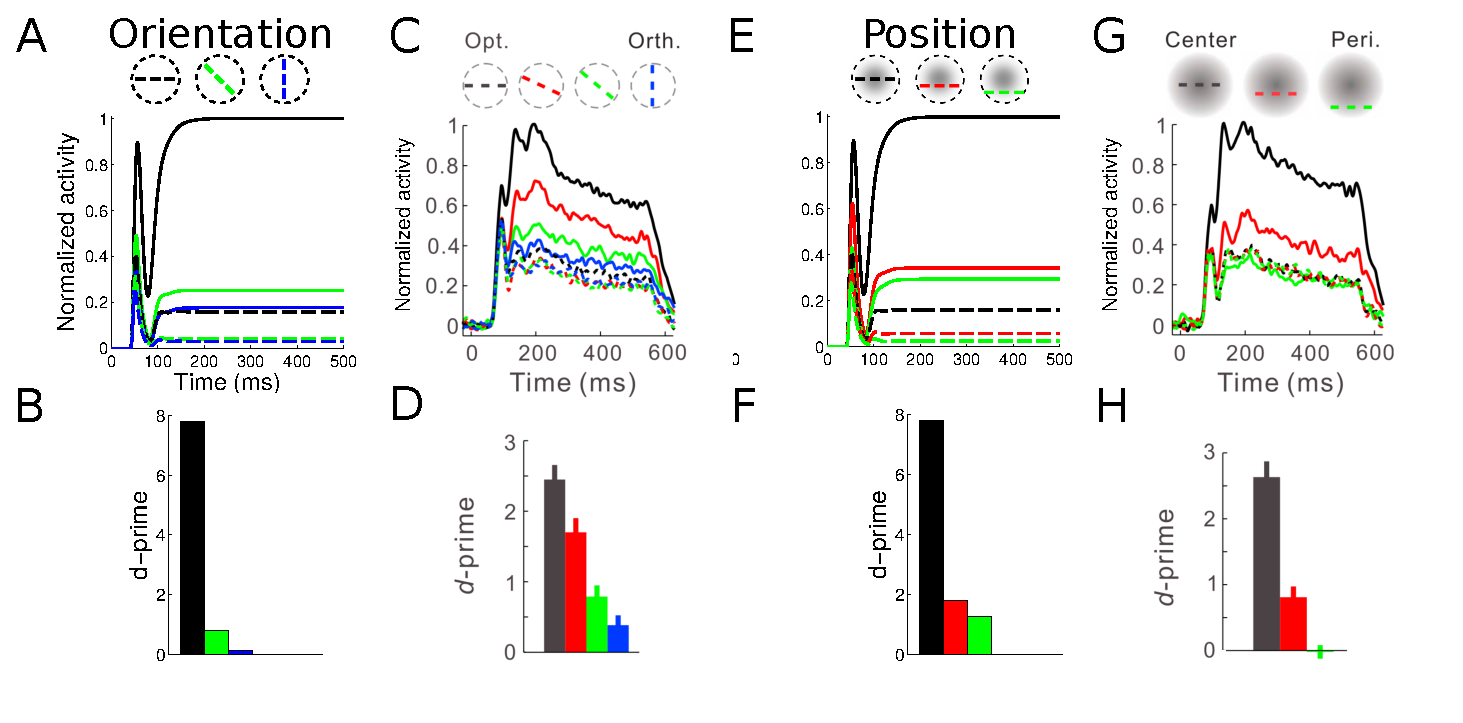
\includegraphics[width=\textwidth]{Contour/figs/FigS1.eps}
\end{center}
\makeatletter
\let\@currsize\normalsize
\caption[Orientation and position dependence of contour integration in V4]{Orientation and position dependence of contour integration in
  V4 $G_c$ cells. The top row shows neuronal responses and the bottom
  row the contour-response $d'$.  Line colors for each figure are
  indicated by the legends at the top of each column. Top row, solid
  lines indicate responses for the 7-bar contour pattern, while dashed
  lines indicate responses for the 1-bar noise pattern.  Note that
  orientations were changed in variable steps based on the tuning
  curve of the neuron under study in the experimental data
  (panels~C,~D) while our simulation only allowed steps of
  $\pi/4$ (panels~A,B).  (A and B) Model results, orientation
  dependence.
 The neuronal responses (A) and the contour-response $d'$
  (B) decreased when the contour was rotated away from the preferred
  orientation. (C and D) Analogous experimental results, adapted from
  \cite{Chen_etal14}.
  (E and F) Model
  results, position dependence.
 The neuronal responses (E) and
  contour-response $d'$ (F) decreased when the contour was translated away from the center of the V4 RF.
  (G and H) Analogous experimental results, adapted from \cite{Chen_etal14}. Panels C, D, G, and H are modified from Figure~3 of~\cite{Chen_etal14}.}
\label{Fig:V4_total}
\end{figure}

\begin{figure}[t]
\begin{center}
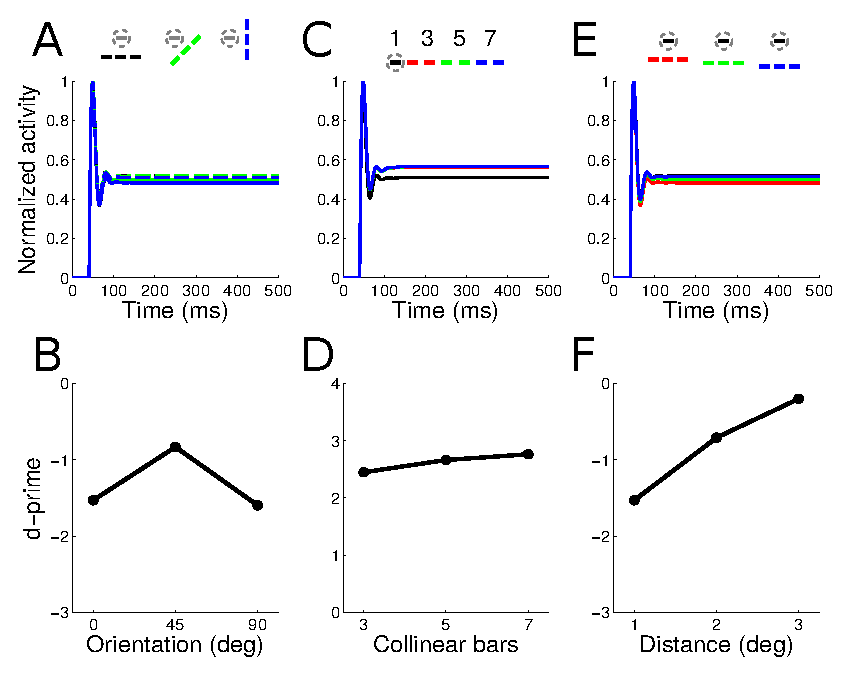
\includegraphics[width=\textwidth]{Contour/figs/FigS2.eps}
\end{center}
\makeatletter
\let\@currsize\normalsize
\caption[Orientation and position dependence of contour integration in V1]{Orientation and position dependence of contour integration in
  V1 $E$ cells, model results. The top row shows neuronal responses
  and the bottom row the contour-response $d'$. Line colors for each
  figures are indicated by the legends at the top of each column. (A
  and B) Orientation dependence of background suppression. The
  neuronal responses (A) and the contour-response $d'$ (B) increased
  for intermediate orientations of the background contour.
  In (A), solid and
  dashed lines correspond to the 7-bar contour and 1-bar noise patterns, respectively.
  (C and D) Contour integration on one end. The neuronal responses (C)
  and contour-response $d'$ (D) increased when bars were added to only
  one side of the V1 RF. (E and F) Position dependence of background
  suppression.  The neuronal responses (E) and contour-response $d'$ (F) increased (approached zero) when the background contour was moved away from the center of the V1 RF.}
\label{Fig:V1_total}
\end{figure}

%%% Local Variables:
%%% mode: latex
%%% TeX-master: "../root"
%%% End:

\end{appendices}

%% REFERENCES

% if you use BIBTEX
\cleardoublepage % add bibliography to TOC
\phantomsection
\addcontentsline{toc}{chapter}{Bibliography}

\bibliographystyle{plainnat}
\bibliography{niebase,niebase_supp} % include niebase_supp for other references

%% bh Add CV to end of file (uncomment to include)
%\makeatletter % needed to make TOC link correctly to CV
%\newcommand*{\@pdfpagephantomchapter}[2][]{\edef\@currentHref{\AM@linkname.\AM@page}\addcontentsline{toc}{chapter}{#1}}
%\makeatother
%
%\includepdf[pages=-,link,linkfit=FitH,addtotoc={1, pdfpagephantomchapter, 1, Curriculum Vitae, CV}]{CV/CV_Brian_Hu.pdf}


\end{document}

%%% Local Variables:
%%% mode: latex
%%% TeX-master: t
%%% End:
